
%%
%% This is file `thesis.tex',
%% generated with the docstrip utility.
%%
%% The original source files were:
%%
%% nudtpaper.dtx  (with options: `thesis')
%% 
%% This is a generated file.
%% 
%% Copyright (C) 2020 by Liu Benyuan <liubenyuan@gmail.com>
%% 
%% This file may be distributed and/or modified under the
%% conditions of the LaTeX Project Public License, either version 1.3a
%% of this license or (at your option) any later version.
%% The latest version of this license is in:
%% 
%% http://www.latex-project.org/lppl.txt
%% 
%% and version 1.3a or later is part of all distributions of LaTeX
%% version 2004/10/01 or later.
%% 
%% To produce the documentation run the original source files ending with `.dtx'
%% through LaTeX.
%% 
%% Any Suggestions : LiuBenYuan <liubenyuan@gmail.com>
%% Thanks Xue Ruini <xueruini@gmail.com> for the thuthesis class!
%% Thanks sofoot for the original NUDT paper class!
%% 
%1. 规范硕士导言
 \documentclass[master,ttf]{nudtpaper}
%2. 规范博士导言
% \documentclass[doctor,twoside,ttf]{nudtpaper}
%3. 建议使用OTF字体获得较好的页面显示效果
%   OTF字体从网上获得,各个系统名称统一。
%   如果你下载的是最新的(1201)OTF英文字体,建议修改nudtpaper.cls,使用
%   Times New Roman PS Std
% \documentclass[doctor,twoside,otf]{nudtpaper}
%   另外,新版的论文模板提供了方正字体选项FZ,效果也不错哦
% \documentclass[doctor,twoside,fz]{nudtpaper}
%4. 如果想生成盲评,传递anon即可,仍需修改个人成果部分
% \documentclass[master,otf,anon]{nudtpaper}
%
%5. 参考文献若用biblatex生成,则使用biber选项
% \documentclass[master,biber]{nudtpaper}
%
%6. 简历中的论文和成果用biblatex参考文献方式生成,则使用resumebib选项
% \documentclass[master,biber,resumebib]{nudtpaper}
%
%\documentclass[doctor,twoside,biber,resumebib,fz]{nudtpaper}
\usepackage{mynudt}
% my package
\newcommand\FIXME[1]{\textcolor{red}{FIX:}\textcolor{red}{#1}}
\usepackage{slashed}




\classification{TP957}
\serialno{0123456}
\confidentiality{公开}
\UDC{}
\title{基于深度学习的气动流场快速精确预测}
\displaytitle{国防科技大学学位论文\LaTeX{}模板}
\author{张三}
\zhdate{\zhtoday}
\entitle{How to Use the \LaTeX{} Document Class for NUDT Dissertations}
\enauthor{ZHANG San}
\endate{\entoday}
\subject{通信与信息工程}
\ensubject{Information and Communication Engineering}
\researchfield{自动目标识别与模糊工程}
\supervisor{李四\quad{}教授}
\cosupervisor{王五\quad{}副教授} % 没有就空着
\ensupervisor{Prof. LI Si}
\encosupervisor{} % 没有就空着
\papertype{工学}
\enpapertype{Engineering}
% 加入makenomenclature命令可用nomencl制作符号列表。

\begin{document}
\graphicspath{{figures/}}
% 制作封面,生成目录,插入摘要,插入符号列表 \\
% 默认符号列表使用denotation.tex,如果要使用nomencl \\
% 需要注释掉denotation,并取消下面两个命令的注释。 \\
% cleardoublepage% \\
% printnomenclature% \\
\maketitle
\frontmatter
\tableofcontents
\listoftables
\listoffigures

%如果不是送审论文,则将true改为false即可
\newif\ifreview\reviewfalse

\midmatter
\begin{cabstract}

气动优化设计是航空航天飞行器设计等应用的重要组成部分,随着飞行器产业的发展和应对复杂现实环境需求的提升,
气动优化往往涉及许多相互交织影响的因素,容易导致设计优化空间“爆炸”。全阶的计算流体力学(CFD)方法能够针对特定流动状态进行高精度的模拟,但往往耗时较长难以进行全面的设计空间探索;虽然基于传统机器学习方法的优化技术在构建代理模型、降阶模型等方面有广泛的应用,
但这类方法多适用于简单气动优化问题,具有一定的局限性。
近年来,深度学习相关研究不断深入并推动诸多应用领域进一步发展,为提升气动优化效率,
构建高效、准确的气动评估方法提供了新的途径。本文主要研究内容如下:

\begin{itemize}
	\item[(1)] 通过对比研究气动流场模拟任务和图像回归预测任务的相似性和不同点,本文提出了一种基于深度卷积网络的气动流场预测方法。首先,针对流场数据的表示问题,提出基于笛卡尔网络的流场数据表示方法,将流场数据转化为深度神经网络可以接受的形式。
	其次,针对边界层等区域流场物理量变化大、包含重要信息多特点,本文提出了嵌入注意力模块的深度卷积网络,能够有效学习该区域流动规律,提升模型预测准确率;基于流体运动遵循的质量守恒定律和动量守恒定律,设计了物理约束的损失函数,有效保证了深度学习预测模型预测结果和CFD求解器的物理一致性。为了全面的评估气动流场预测模型的性能,本文定义了新的性能指标,在测试集上的对比试验结果表明该方法能有效提升气动流场模拟效率,同时将预测误差控制在5\%以内。
	\item[(2)] 针对深度卷积网络难以处理非欧式空间流场数据的问题,本文提出了一种基于图神经网络的气动流场模拟加速方法。
	基于图结构对流场数据进行表示,能够有效减少数据转换过程中的信息丢失,实现流场几何外形、边界条件和流动控制变量的有效融合;
	基于图卷积网络的流模拟加速模块能够提取流场数据特征,为CFD求解器提供接近收敛状态的初始场,减少CFD迭代计算的时间。
	实验结果表明该方法能够在加速气动流场模拟的同时,从根本上保证了模拟结果的有效性。
	
\end{itemize}

本文针对飞行器气动优化设计中的典型问题,基于深度学习技术和方法,提出针对流场数据的表示方法,搭建气动流场预测模型和气动流场模拟加速模型,通过嵌入物理约束和融合传统CFD方法进一步优化模型预测结果,有效提升气动流场模拟效率,为基于深度学习的智能气动流场和气动性能预测技术在复杂飞行器气动优化设计中的应用奠定基础。

\end{cabstract}
\ckeywords{气动优化; 计算流体力学; 深度学习; 图神经网络; 物理一致性}



\begin{eabstract}
National University of Defense Technology is a comprehensive national key university based in Changsha, %
Hunan Province, China. It is under the dual supervision of the Ministry of National Defense %
and the Ministry of Education, designated for Project 211 and Project 985, %
the two national plans for facilitating the development of Chinese higher education. %

NUDT was originally founded in 1953 as the Military Academy of Engineering in Harbin of Heilongjiang Province. %
In 1970 the Academy of Engineering moved southwards to Changsha and was renamed Changsha Institute of Technology.%
 The Institute changed its name to National University of Defense Technology in 1978.

\end{eabstract}
\ekeywords{Aerodynamic Optimization; Computational Fluid Dynamics; Deep Learning; Graph  Neural  Network; Physical Consistency}


\input{data/denotation}

%书写正文,可以根据需要增添章节; 正文还包括致谢,参考文献与成果
\mainmatter

\chapter{绪论}
CFD数值模拟在航空航天飞行器气动优化设计等应用中发挥着重要作用,
但是全阶CFD模拟经济、时间成本高昂,限制了设计人员进行全面、快速的设计空间探索和设计迭代。为了以更省时省力、又快又好地获得最优解,机器学习等智能算法和技术在气动优化的寻优算法及构建代理模型、降阶模型等方面有广泛的应用,但是传统机器学习方法适用于处理低维数据,难以推广到复杂的CFD应用场景。随着人工智能领域的快速发展,以深度学习为代表的智能方法和技术在处理高维复杂数据上展现了强大的学习能力,从而为快速、精确气动评估提供了新思路和新方法。



\section{研究背景及意义}
计算流体力学( Computational Fluid Dynamics,CFD )
作为了解和探索流体运动的手段,在航空航天,交通运输,石油勘探,天气预测,水利工程和石油化工等工程领域发挥着极其重要的作用。近年来,随着计算机性能的提升,CFD的应用前景进一步扩大,渗透到生活的方方面面。小到吸管设计,大到汽车制造,生活中随处可见CFD的身影。在2020年新冠疫情期间,CFD研究者通过对喷嚏飞沫的流动状态进行研究,得出喷嚏飞沫可以漂浮8米远的结论,为疫情防控做出了重要的贡献\cite{JAMA-喷嚏}。

复杂飞行器气动优化设计是CFD的重要应用领域,以增升减阻为目标的气动优化是飞行器设计的重要组成部分。
如文献\cite{增升减阻ep}指出,对于某民航客机,起飞升阻比每提高1\%,可增加14个乘客;
着陆最大升力系数每增加1\%,则可增加22个乘客。
由此可见,提升气动优化效率,实现快速、精准的气动评估对于推动飞行器设计发展具有重要意义。
尽管传统的全阶CFD数值模拟可针对特定状态获得较高精度的评估结果,但是时间、经济等成本巨大。
为了以更省时省力、又快又好地获得最优解,许多研究者在优化设计时对原始模型进行简化处理,包括采用更为简单的代理模型\cite{代理模型}和降阶模型\cite{降阶模型},代替复杂的CFD评估过程,减少计算开销;引入基于机器学习的智能方法和技术等。因此,在保证模拟精度的基础上,不断地提升气动模拟的效率是数值模拟领域现阶段的研究热点,具有极大的实际应用价值。然而加速和优化气动评估目前面临着以下挑战:

\vspace{-0.2cm}
\begin{itemize}
	\item[(1)] 气动优化往往涉及许多相互交织影响的因素。以常见的超临界机翼优化为例,除需考虑巡航升阻力系数、升阻比、力矩系数等设
	计点性能外,抖振、阻力发散等非设计点动态特性也需考虑;同时,优化还存在一些必要约束,如机翼厚度、油箱容积、前后缘装置等。海量设计参数容易导致设计空间“爆炸”,仅依靠传统的CFD数值模拟极大地限制了对复杂飞行器进行全面的设计空间探索。
	\item[(2)] 机器学习等智能算法和技术,通过部分或者全部代替复杂的CFD评估过程,在原始模型简化处理方面有广泛的应用。
	然而,大部分机器学习技术借助于发展成熟的机器学习方法和技术,属于浅层学习方法,随着CFD所模拟的问题越加的复杂,其预测精度和应用范围相对有限。
	此外,传统机器学习算法复杂度将随着样本数量和模
	型精度的提高呈指数级增长,目前应用范围多限于一些容易获得训练样本的二维简单优化
	问题。

\end{itemize}

自2006年Hinton等提出深度信念网络\cite{深度信念网络}以来,在GPU、TPU等高性能计算机硬件的助力下,
以深度学习为代表的智能方法和技术迅速发展,成功应用于图像分类与识别,医疗诊断,视频预测,自然语言处理等诸多领域。
在学术界,深度学习算法和技术包括其相关应用也是世界各大研究实验室和顶尖大学的研究热点,
比如斯坦福大学、纽约大学、加拿大蒙特利尔大学等成为研究深度学习的重镇,在国际顶尖会议和期刊上涌现了许多关于深度学习的研究内容;
在工业界,包括众多互联网公司在内的知名企业专门设立了深度学习实验室,促进深度学习技术转化落地。

由于采用了复杂和更深层次的模型结构,深度学习模型更善于从数据中提取特征,而不是依靠人工构建特征,极大提升了归纳能力,
能够自主进行特征选择,可以从大量的候选特征中剔除无用特征再进行回归和分类,具备
深层次学习能力,尤其适合于归纳、分析高维、时空相关的流场数据,展现出广阔的应用前景。

一方面,深度学习方法拥有巨大的潜力解决CFD领域所面临的问题;另一方面,
基于深度学习的气动评估及其在气动优化中的应用尚处于起步阶段,已有应用多为二
维简单外形算例,多参考深度学习在其他领域应用较为成熟的方法技术,尤其是深度卷积
神经网络在计算机视觉领域的研究成果,深度学习还没有与空气动力学实现交叉融合。
因此,研究基于深度学习的气动优化技术对于解决气动优化领域所面临的问题和满足设计空间探索的实际需求具有重大意义。



\section{研究现状}
如图\ref{fig:1}所示,早在20世纪70年代就出现气动优化的应用,相关研究主要聚焦于使用小扰动方程、全势流等快速方
法进行气动评估\cite{70年代1,70年代2},结合梯度类优化算法对气动性能进行优化。
在20世纪80年代,以遗传算法为代表的进化类算法和以蚁群算法与模拟退火为代表的启发式算法
逐渐得到应用\cite{2000Aerodynamic,Genetic,Obayashi1995Genetic},这类方法不需要引入梯度信息,因其优化过程具有随机性,使用者无需关心优化的细节,所以在当时被广泛应用到气动优化过程。
但是,进化类算法依赖大量适应度函数分析,优化效率较低。
伴随方法\cite{Jameson2000Aerodynamic}的提出再次推动了基于梯度的优化方法的发展,通过求解伴随场,有效提升了求解梯度的效率。
为了结合两类算法的优点,混合算法在2000年以后开始得到广泛应用,实现局部寻优和全局寻优能力的均衡,通过将优化分阶段提高搜索效率等。

\begin{figure}[htp]
	\centering
	%\includegraphics[width=0.42\textwidth]{data/MLP.pdf}
	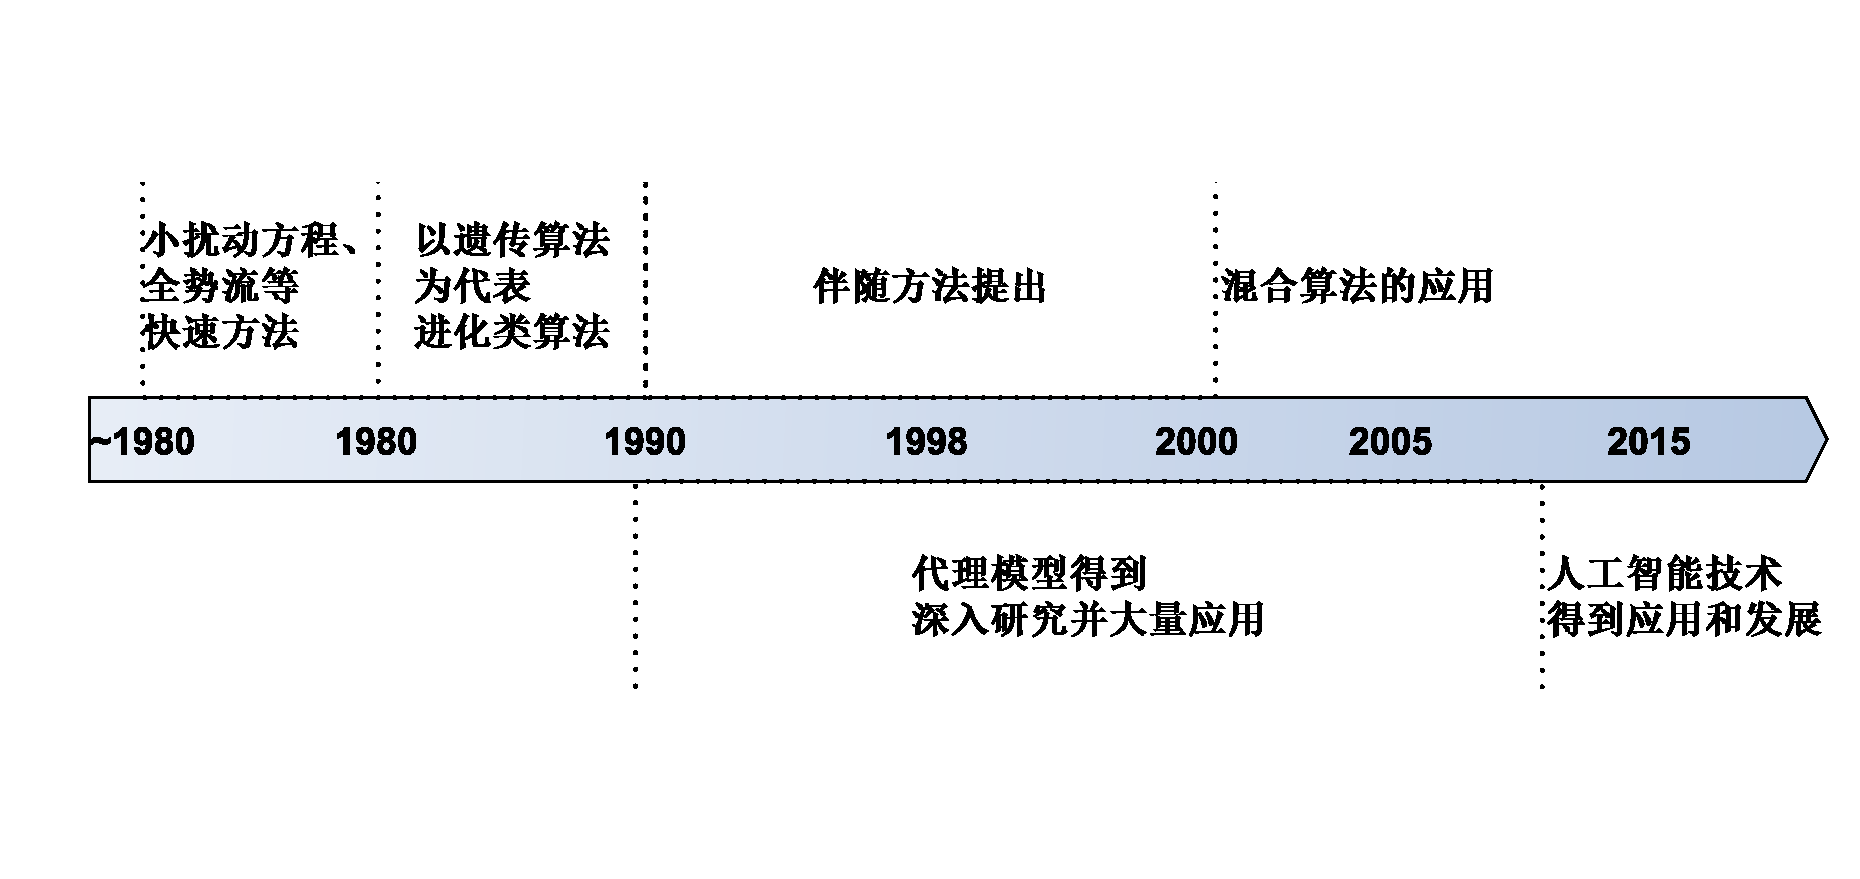
\includegraphics[width=0.92\textwidth]{figures/develop.pdf}
	\caption{气动优化技术的发展历程}
	\label{fig:1}
\end{figure}

随着机器学习技术和人工神经网络的发展,许多学者对以智能学习为基础的气动流场和气动性能预测方法进行了大量研究,基于智能学习的气动优化也是领域研究热点和本文关注的重点。
通过总结相关文献,本文对基于智能学习的气动优化技术和研究进行了整理和分类。
如图\ref{fig:智能优化}所示,基于智能学习的气动优化技术概括而言主要有两种:
一是利用传统机器学习方法和技术构建优化器、代理模型、降阶模型来减少计算开销,采用数据驱动方式,
通过对大量训练样例的“学习”构建数据间内部关系的模型,对未知数据进行预测;
二是基于深度学习方法和技术对气动特性和气动性能进行预测,利用深度神经网络强大的归纳学习能力,
提取高维、时空相关流场数据中的重要信息,构建气动流场、气动性能快速预测模型。

\begin{figure}[htp]
	\centering
	%\includegraphics[width=0.42\textwidth]{data/MLP.pdf}
	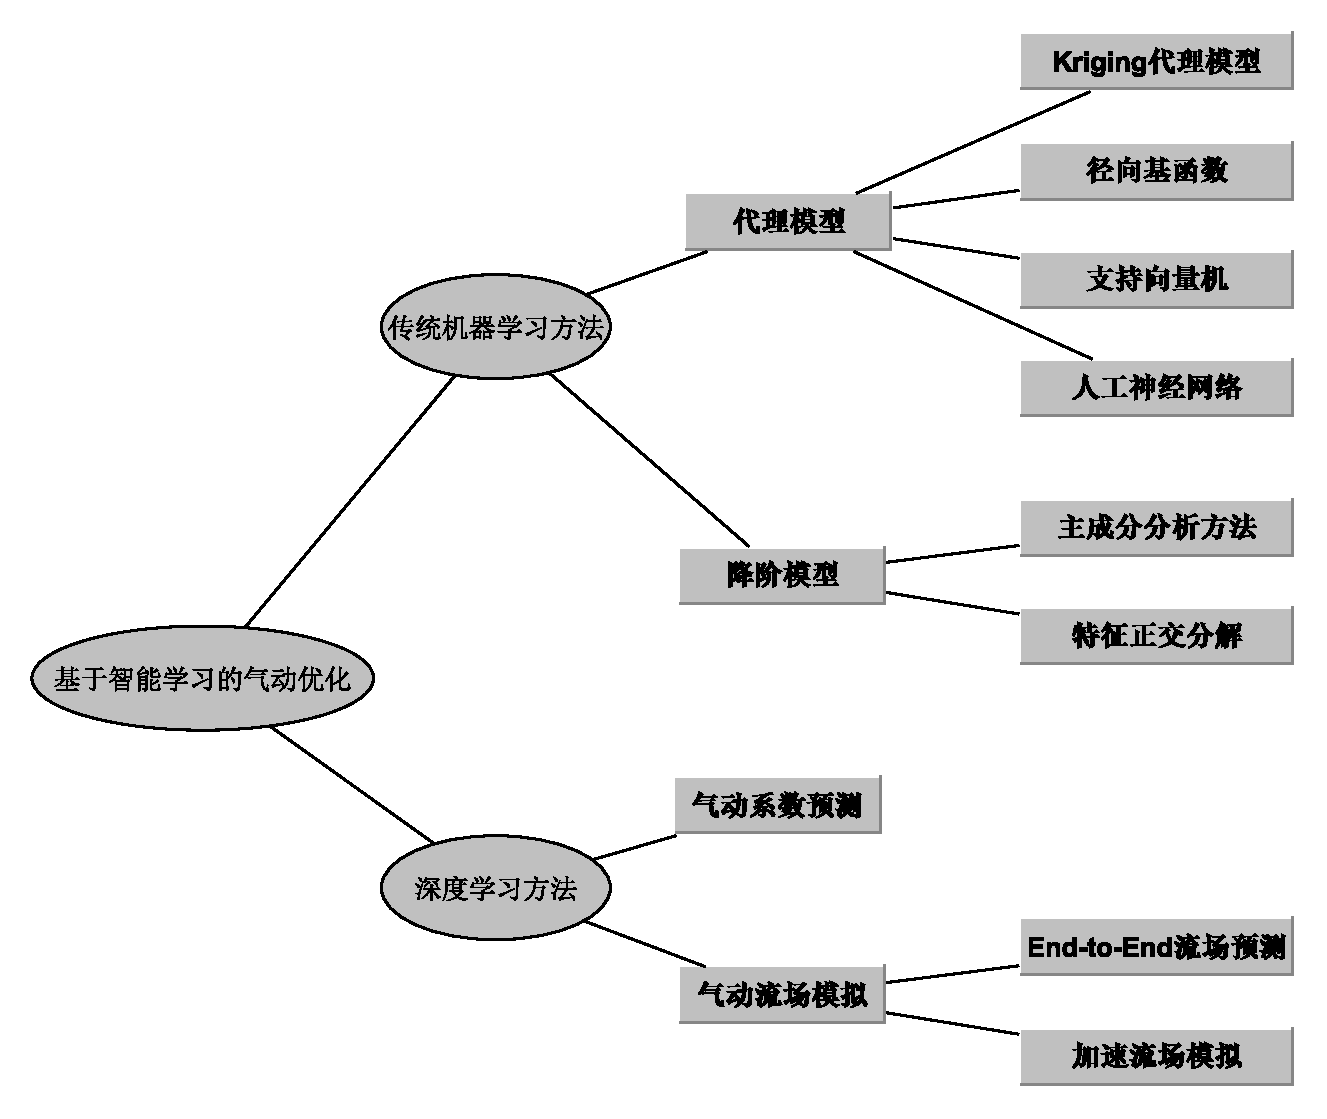
\includegraphics[width=0.92\textwidth]{figures/aicfd.pdf}
	\caption{基于智能学习的气动优化技术}
	\label{fig:智能优化}
\end{figure}

\subsection{基于传统机器学习的气动优化}
传统机器学习方法在气动优化中最典型的应用就是基于响应面法(response surface methodology,RSM)、多项式回归函数(Polynomial Regression,PR)、径向基函数(Radial Basis Functions,RBF)和人工神经网络(Artificial Neural Networks,ANN)等方法构建模型,快速从已计算的样本中预测设定的目标函数,从而达到代替CFD数值模拟的效果。此类优化方法通常被称为基于代理模型的优化方法。

Kanazaki和Tanaka等人\cite{Kanazaki2007Multi}针对飞机降落和接近失速条件下机翼升力系统的设计和优化问题,首先利用基于雷诺平均Navier-Stokes的CFD方法获取训练样本,设计了基于克里格(Kriging)代理模型的最大化升力系数的目标函数,实验结果表明相对于传统的遗传算法克里格模型显著降低了计算开销,同时实现了更好的性能。此外,作者还利用数据挖掘中的方差泛函分析方法分析了影响升力系统设计的主要因素。

张彬乾和罗烈等人\cite{张罗}针对飞翼布局设计中气动与隐身设计矛盾更为突出的问题,采用高精度气动和隐身计算方法,利用RBF神经网络代替复杂目标函数的评估,结合遗传算法和松散式代理模型管理方法,建立了翼型多目标优化设计平台。实验结果证明基于RBF神经网络的代理模型能有效模拟和评估翼型等几何形状与气动和隐身特性之间存在的强烈非线性关系。

Ju和Zhang等人\cite{Ame}为了解决蒙特卡罗模拟方法耗时长、计算开销大的问题,深入比较了人工神经网络、径向基函数和支持向量机模型(Support Vector Machine,SVM)的拟合精度,结果表明SVM精度较高,并以此基于SVM、遗传算法和蒙特卡罗方法针对翼型表面粗糙度的不确定性对翼型升阻系数进行了鲁棒性优化,实验结果表明,遗传算法-支持向量回归模型可以很好地捕获从表面粗糙度到机翼气动性能的不确定性传播。

基于代理模型的方法主要关注在给定输入数据的条件下,模型预测结果的准确性。
当研究输入变量之间的关系或者代理模型难以处理高维数据时,往往需要借助以主成分分析( Principal Component Analysis,PCA )和特征向量分解( Poper Orthogonal Decomposition,POD )为代表的机器学习方法。
比如,Kapsoulis和Dimitrios等人\cite{Kapsoulis2018Evolutionary}针对气动优化中维数灾难问题,整合进遗传算法和PCA方法,
在交叉和变异阶段使用PCA对设计变量进行降维,在降低优化复杂度的同时促使新个体的变化方向
沿着方差最大的方向进行,以提高优化效率。
此外,PCA和POD还可以用来对偏微分方程组进行降阶,得到降阶模型,再结合基于代理模型的方法,直接对气动流场进行预测。

\subsection{基于深度学习的气动优化}
近年来,以深度学习为代表的人工智能技术取得了令人瞩目的发展和成就,
深度学习等智能方法、技术也为快速、精确气动评估提供了新手段。
根据气动优化的目标不同,可以将基于深度学习的气动优化技术分为气动系数预测技术和气动流场模拟技术。
气动系数预测技术利用深度神经网络对感兴趣的气动系数(比如飞行器升力系数,升阻比等)进行回归预测,不关心流体在流场中运动的细节,属于深度学习在气动优化中的浅层运用。

Zhang和Sun等人\cite{LiftCoefficient}探讨了卷积神经网络技术的适应性以实现空气动力学元建模任务。
针对可变的流动条件和物体的几何形状,即具有多种形状的翼型,具有多个流动马赫数,雷诺数和攻角的流动条件,
训练了多个卷积神经网络以预测机翼的升力系数。
证明利用深度学习对空气动力学任务进行元建模的有效性。
将卷积神经网络结果与多层感知机的结果进行比较,发现基于卷积神经网络的元建模方法与多层感知机在学习能力方面具有可比性;
更重要的是,在几何表示约束最小的条件下,卷积神经网络模型预测准确性更高。

陈海和钱炜祺等人\cite{陈海2018}提出了一种基于深度学习的翼型气动系数预测方法,有效克服了以往方法依赖翼型设计参数以及算法复杂度随预测精度的提高呈指数级增长等缺点。该方法能够在只给出翼型图像的基础上,使用深度卷积神经网络根据翼型图像对其气动力系数进行了建模。研究结果表明显示模型预测的翼型气动系数获得了较高的精度,说明深度学习在翼型气动系数预测方面具有很好的应用前景。

利用深度学习技术对气动流场进行模拟,研究者可以观察到物理量(比如速度和压力)在流场中的分布,
获取更多有用的信息,对飞行器设计等工作进行针对性的优化和调整。
本文进一步对基于深度学习的流场模拟进行了分类:基于深度学习的流场预测方法和基于深度学习的流场模拟加速方法。
前者使用深度学习技术全部取代CFD过程实现End-to-End(端到端)流场预测,后者将深度学习方法作为加速模块并与传统的CFD求解器进行融合。

在基于深度学习的流场预测方法中,除了在神经网络模型训练阶段,需要利用CFD求解器准备训练数据以外,在模型训练完成后,推理过程不再依赖CFD方法,深度学习模型可以独立地对给定的几何体和流场条件进行预测。近年来,在基于深度学习的流场预测方向涌现了大量工作。

惠心雨和袁泽龙等人\cite{惠心雨2019}为了克服传统CFD计算需要耗费大量的计算时间与成本的缺陷,提出了一种基于深度学习的非定常周期性流场的预测框架,可以实时生成给定状态的高可信度的流场结果。将条件生成对抗网络(Generative Adversarial Networks,GAN)与卷积神经网络相结合,改进条件生成对抗网络对生成样本的约束方法,建立了基于深度学习策略采用改进的回归生成对抗网络模型,并与常规的条件生成对抗网络模型的预测结果进行对比。研究表明,基于改进的回归生成对抗网络的深度学习策略能准确预测出指定时刻的流场变量,且总时长比CFD数值模拟减少至少1个量级。

Guo和Li等人\cite{DBLP:conf/kdd/GuoLI16}针对非一致稳态层流流动建立了基于卷积神经网络(Convolutional Neural Network,CNN)的预测模型,其深度网络架构中包含了卷积编码和卷积解码(Encoder-Decoder)两部分,采用基于笛卡尔网格计算得到的符号距离函数(Signed Distance Function,SDF)作为输入,以LBM(Lattice Boltzmann Methods)求解器的模拟结果(速度场)作为训练样本标签。相对于基于二进制的几何外形表示,SDF值不仅提供了局部几何外形细节,同时包含了全局几何结构的丰富信息。作者针对二维简单形状、包含三维球体和圆柱的管道流等算例速度场进行了训练和预测,获得了较高的精度。深度神经网络预测耗时较GPU平台上LBM模拟快了2个数量级,较CPU平台上LBM模拟则快了4个数量级。该方法可以在早期设计阶段设计迭代中提供快速反馈,为构建实时、交互式设计优化空间探索提供了可能。

在Guo和Li等人的研究基础上,Bhatnagar和Afshar等人\cite{bhatnagar2019prediction}进行了改进,采用类似的深度神经网络架构,以3个翼型、4个雷诺数、21个攻角构成的RANS模拟结果作为训练数据,预测未知翼型、雷诺数、攻角的测试算例的速度场和压力场。与Guo等人的研究不同的是,作者在训练输入中增加了雷诺数、攻角信息( 在深度神经网络的全连接层处输入),且在损失函数中引入了gradient sharpening和L1正则化,提高了模型泛化能力和预测精度。

Miyanawala和Jaiman\cite{2017An}使用CNN预测了不同的阻流体的低雷诺数下的阻流体的空气动力系数。 他们提出了一种使用CNN和随机梯度下降法的数据驱动方法,用于在非定常流动问题中对Navier-Stokes方程进行模型简化。

Lee和You等人\cite{lee2019data}使用深度学习技术对在未获知的雷诺数条件下非定常圆柱绕进行了流场预测,考虑到守恒律对预测性能的影响,评测了GAN和multi-scale CNN等四种深度神经网络的预测效果。实验结果表明,对于短期预测,四种神经网络都实现了较好的预测效果;对于长期预测,考虑物理守恒的GAN和multi-scale CNN相较于不考虑物理守恒的multi-scale CNN实现了更好的性能,不考虑物理守恒的GAN实现了在四种深度神经网络中表现最好。该结果证明GAN深度神经网络充分利用了无监督训练,因此它们可以应用于先验未知的基础物理学的问题。

Filipe和Thomas等人\cite{2020Combining}使用图神经网格对流场进行了预测。基于图神经网络的方法利用网格点之间的拓扑信息和网格点上的特征向量作为输入,训练得到基于网格点的流场(包括速度场和压力场)。此外,该方法还采用粗网格上采样的结果作为输入,引入可导的求解器对粗网格点进行调整,增加了模型的泛化能力。

因为在进行预测时不需要进行耗时的迭代计算,流场预测方法的显著特点是预测效率非常高,但是预测结果的有效性即满足流体运动的规律往往难以得到保证。许多研究者针对基于深度学习的预测结果有效性进行了探索。

Ling和Templeton等人\cite{invariance}针对雷诺平均湍流模型提出了一种基于深度神经网络预测模型TBNN。
该架构使用具有不变张量的乘法层来实现将伽利略不变性嵌入预测的雷诺应力张量。 
实验结果证明了这种神经与通用神经网络相比,预测结果的准确性和物理一致性得到了提升。

Wang和Kashinath\cite{DBLP:journals/nips2019}等人提出了一种新颖的混合深度学习模型TF-Net,该模型将表示学习和湍流仿真技术相结合。TF-Net利用湍流的多尺度行为来设计可训练的尺度分离算子,以分别对不同尺度范围进行建模。 我们提供了TF-Net和基线的详尽比较,并观察到了预测误差和所需物理量(包括散度,
湍流动能和能谱)。采用不同的评估指标来评估深度深度学习模型对物理系统的预测性能包括准确性和物理一致性。


在基于深度学习的流场模拟加速方法中,传统的CFD求解器仍然参与流场模拟的过程,通过使用深度学习模型减少迭代计算量,达到计算流场模拟的效果。
相较于流场预测方法,流场模拟加速方法的模拟效率会有所下降,但是由于CFD求解器参与了流场模拟并且输出了最终了模拟结果,
使得流场模拟结果的有效性得到了充分的保证。具有代表性的工作是文献\cite{cfdnet},
Octavi和Abhinav等人针对流场模拟提出了一种基于深度学习的加速器CFDnet。将稳态流场模拟分为三个部分:基于CFD求解器的warmup,
基于深度学习模型的Inference,基于CFD求解器的Refinement。
在CFD迭代计算过程中初始阶段和最终阶段之间,利用深度神经网络建立映射代替大部分“invalid”迭代计算。
在内插数据集和外推数据集上对CFDnet的效果进行了测试,结果表明,CFDNet满足特定领域物理求解器的收敛约束,同时在层流和湍流模拟方面可达到1.9-7.4x的加速比。 此外,通过测试CFDNet对训练期间看不见的新几何形状的预测来证明其泛化能力。在这种情况下,CFDnet满足CFD求解器的收敛标准,同时收敛速度仍明显优于仅使用传统CFD求解器的对照组。


综上所述,相较于传统机器学习方法,基于深度学习的气动特性和气动性能预测具有以下优势:
1)深度模型可以自适应提取输入特征,无需进行人工筛选和精简,可极大地减少设计变量数目限制。2)深度学习很好地保留了坐标点间的空间相邻关系,其特征提取过程具有空间上的平移不变性和缩放不变性。3)深度学习由于能够提取更深层次的特征,因而拥有更强大的归纳能力,不仅可以获得气动性能预测,还可以将流场特征(如压力分布等)作为预测输出。
但是,使用深度学习技术解决气动流场优化问题,不能是简单的迁移运用,需要根据应用场景的不同,在流场模拟效率、模拟结果精度和有效性等方面进行优化,又快又好地解决气动优化问题。

\section{主要工作和创新点}
本文在深入分析现有基于智能学习的气动优化技术的基础上,受到深度卷积网络和图神经网络在计算机视觉领域成功应用的启发,将其引入来提升气动评估的效率。
本文侧重对稳态流动(即达到稳定状态后,流体中压力,速度等物理量都不随时间变化)问题的研究,
针对现有工作将深度学习技术应用到气动优化领域的一些不足,在流场数据表示,网络架构搭建与优化,嵌入物理模型约束和性能评价指标等方面展开相关研究。本文贡献了两个测试数据集,用于测试与分析基于不同深度学习网络的气动优化方法,并得到相应结论。
总结而言,本文的主要工作和创新点如下:
\begin{itemize}
	\item[(1)] 提出了一种基于深度卷积网络(Deep Neural Networks,DNN)的气动流场预测方法。
	首先,针对深度网络的输入数据的表示问题,提出了针对流场流场数据的特征表示方法;利用基于LBM(Lattice Boltzmann Method)的数值模拟求解器构造了两种不同流动条件下的数据集;
	其次,基于图像分割领域的深度网络模型,设计了适用于流场预测的网络架构,同时引入了注意力机制和神经网络剪枝技术,分别对模型的预测精度和推理速度进行了优化;
	研究流体流动的特性,基于质量守恒和动量守恒的控制方程,设计了嵌入物理模型约束的损失函数。
	在性能评价指标方面,除了深度学习训练常用的相对评价误差以外,本文提出了新的评价指标用来评估气动预测模型在感兴趣区域(Region of  interest,RoI)和物理守恒性等方面的预测效果。
	实验结果表明该方法能够对给定的输入数据进行快速的预测,相较于LBM求解器预测速度提升了四个数量级,同时保证预测误差低于5\%。
		
	
	\item[(2)] 提出了一种基于图神经网络(Graph Neural  Networks,GNN)的气动模拟加速方法。
	首先,利用网格生成软件生成的网格文件,基于算例的边界条件设置,构造了带有拓扑信息和节点特征信息的图结构输入数据,用于训练图神经网络;
	其次,利用图卷积网络(Graph  Convolutional Network,GCN)构建气动模拟的加速模块。
	完成模型训练后,将模型的推理结果反馈给CFD求解器,为求解器迭代计算过程提供一个更接近于稳定状态的初场,减少CFD的模拟时间。
	实验结果表明,基于GNN的气动模拟加速方法能够有效提升流场模拟的效率,此外,通过CFD求解器对GCN的模拟结果进行优化,保证了模拟结果的预测一致性。
	
	
	
\end{itemize}

\section{论文结构}
本文主要研究基于深度学习方法和技术的气动流场模拟方法,利用深度神经网络和图神经网络设计实现了气动流场的预测方法和模拟加速方法,论文的主要结构如下:

第一章:主要介绍了传统CFD模拟在实际工程应用中遇到的挑战,智能学习方法和技术在气动优化方向的研究现状以及论文的主要工作。

第二章:通过分析传统CFD模拟流程定义了研究问题,介绍了计算流体力学相关理论基础;针对第三章、第四章研究内容,
重点介绍了相关的深度学习知识与技术,包括常用的深度卷积网络模型和图神经网络模型。

第三章:介绍基于深度卷积神经网络的气动流场预测方法,提出针对流场数据的表示方法。
基于图像分割网络设计气动流场预测架构,通过嵌入注意力模块和设计嵌入物理约束的损失函数对流场预测模型进行针对性的优化。
介绍利用CFD求解器生成实验数据集的流程,定义新的流场预测结果的评价指标。
通过实验和结果分析,对模型预测结果的准确率、有效性以及流场模拟效率进行了全面的评估。

第四章:介绍基于图神经网络的气动流场模拟加速方法,提出基于图结构的流场数据表示方法,
基于图卷积网络设计气动流场模拟加速模块,利用CFD求解器对模型模拟结果进行优化,
在提升流场模拟效率的同时保证流场模拟结果的有效性。
在测试集上对提出的方法进行实验论证,分析实验结果。

第五章:对本文的工作进行总结和评价,分析现有研究工作的不足和缺陷,对未来的研究方向和研究内容进行展望。












\chapter{研究基础与相关技术}

近年来,深度学习一直是计算机领域乃至多学科交叉应用领域的研究热点,不仅在计算机视觉方向有着广泛的应用,在光学、材料和航空航天等领域也出现了相关研究。尤其对于大数据应用场景,基于深度学习的方法已经成为重要的数据挖掘手段。
对于气动优化乃至整个CFD领域而言,深度学习方法在此领域获得发展并取得成功只是时间问题。
为了便于阐述本课题工作,本章首先定义了本课题要解决的问题,即明确利用深度学习方法和技术要解决的问题和要达到的效果;
其次介绍了CFD相关的基础理论,主要包括建立在宏观层次的Navier-Stokes(N-S)方程和介观层次的格子Boltzmann方法(Lattice Boltzmann Methods,LBM);最后介绍了四种与本文工作紧密相关的深度神经网络和图神经网络模型。

\section{研究问题定义}
利用传统CFD方法对流体问题(包括气动优化问题)进行研究的流程如图\ref{fig:cfdflow}所示。
\begin{figure}[htp]
	\centering
	%\includegraphics[width=0.42\textwidth]{data/MLP.pdf}
	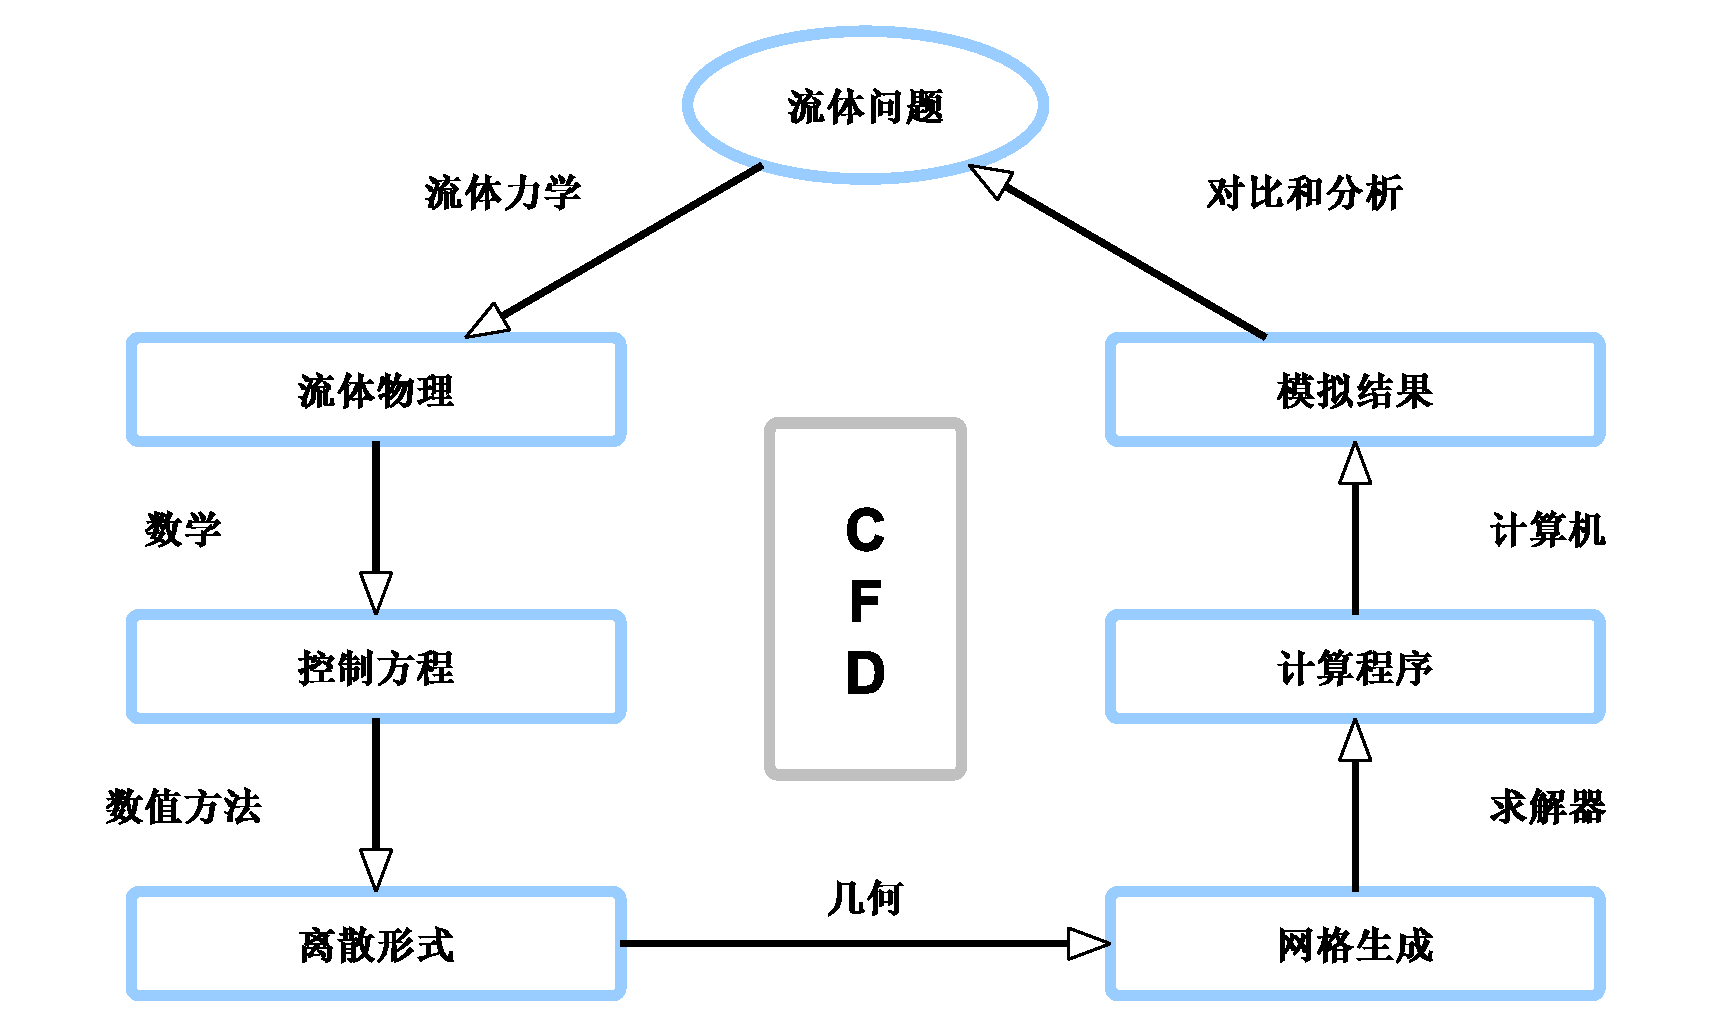
\includegraphics[width=0.92\textwidth]{figures/cfdflow.pdf}
	\caption{利用传统CFD方法研究和解决流体问题的流程示意图}
	\label{fig:cfdflow}
\end{figure}


首先利用流体力学知识对流体问题进行理论分析,建立物理模型;
根据流体运动遵循的基本规律,利用数学方法推导出流体流动的控制方程,
宏观层面上有粘性流动的Navier-Stokes方程和无粘流动的欧拉方程;
针对特定的流体问题,明确其物理基础和假设,简化控制方程、确定边界条件和初始条件。
由于CFD方法是利用数值计算对流体流动进行模拟,所以研究的不是连续运动的流体,必须利用数值方法对时间和空间进行离散,
以便进行迭代计算求解。对空间的离散方法包括有限差分方法,有限元方法和有限体积方法;
对时间的离散通常包括适用于定常流体问题求解的显示方法和适用于非定常问题的求解的隐式方法。
确定离散形式之后,需要对几何进行划分,即生成网络,在网格上对控制方程进行求解。
网格生成之后,选择合适的CFD求解器,依据初始条件和边界条件对求解器的参数进行设置,
最后利用计算机进行迭代计算至模拟结果收敛。



这种全阶CFD模拟往往耗时较长,难以满足全面、快速的设计空间探索需求。
为了加速CFD模拟进程,提升气动优化效率,本文针对二维稳态流动问题,
提出了两种基于深度学习的气动优化模型,图\ref{fig:cfd_dnnflow}展示了这两种模型的工作流程。

\begin{figure}[htp]
	\centering
	%\includegraphics[width=0.42\textwidth]{data/MLP.pdf}
	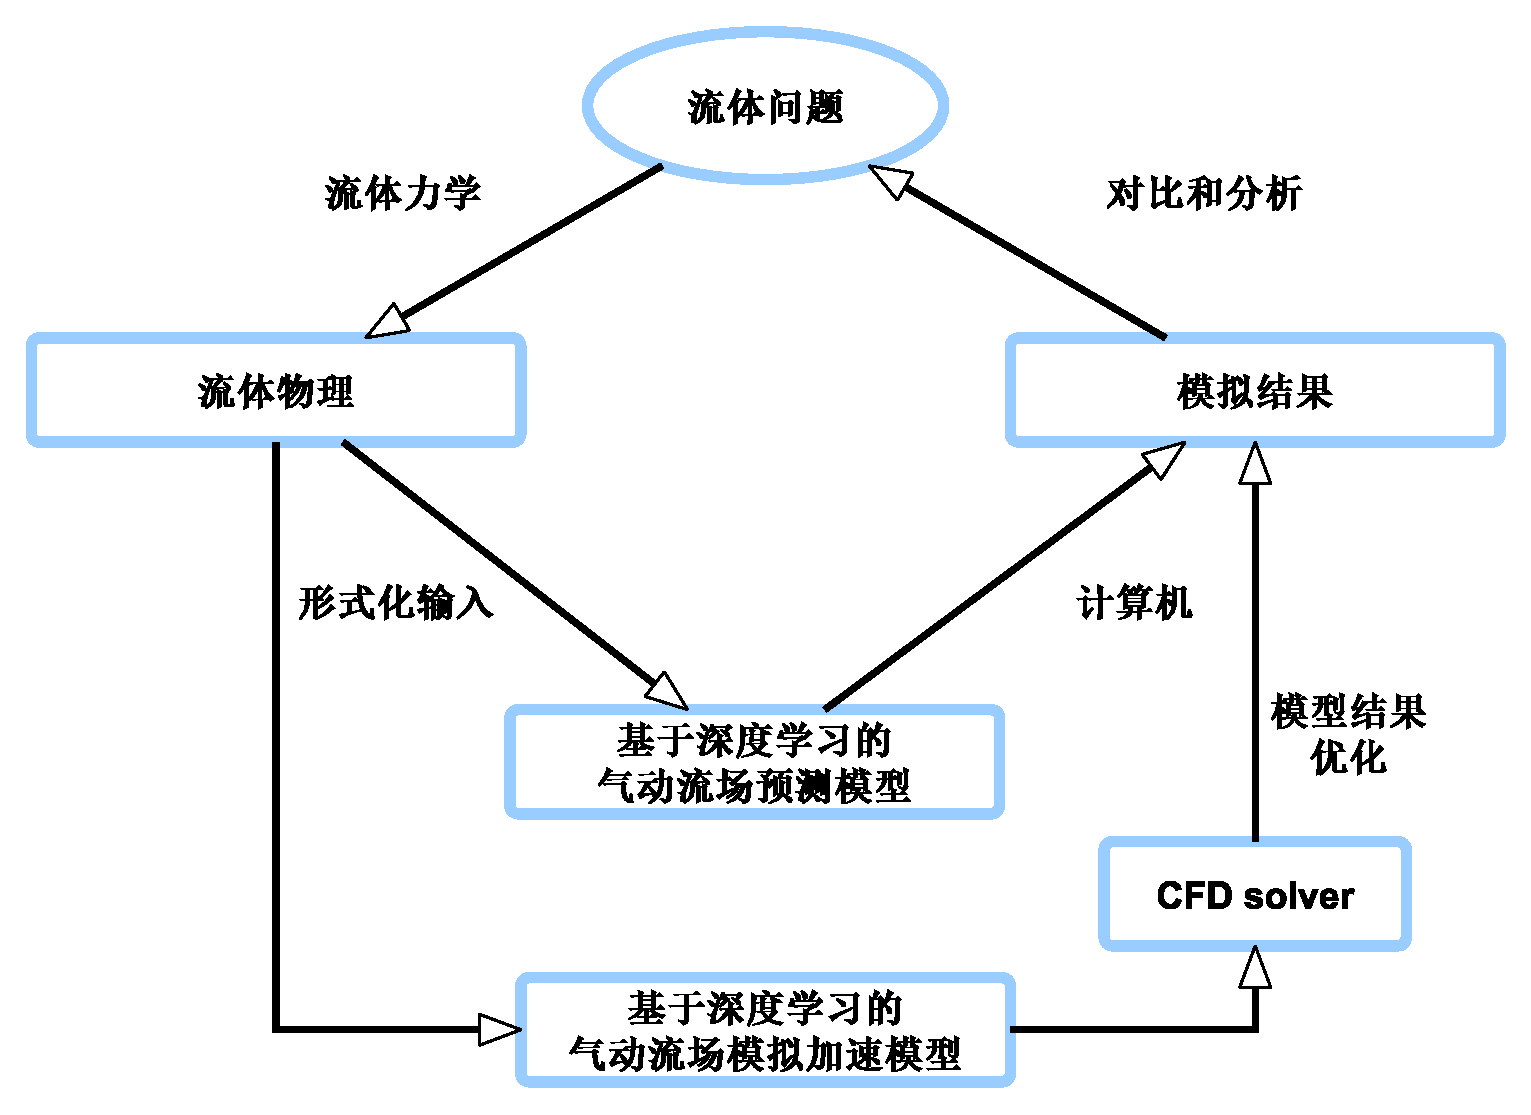
\includegraphics[width=0.92\textwidth]{figures/cfd_dnnflow.pdf}
	\caption{基于深度学习的气动优化模型工作流程示意图}
	\label{fig:cfd_dnnflow}
\end{figure}

在气动流场预测模型中,将边界条件和几何外形形式化为适合神经网络训练的输入,
利用深度学习方法构建端到端的预测模型,通过神经网络正向推理过程,得到对应的气动流场预测结果;
气动流场模拟加速模型的流程与气动流场预测模型类似,不同之处在于模型训练完成后,将深度学习模型的结果输入到CFD求解器中,为CFD求解过程提供一个更加接近收敛状态的初场,从而达到减少迭代计算量、加速模拟的效果。



\section{计算流体动力学基础理论}
根据对气体在不同尺度上动力学规律的描述,计算流体力学方法可分为三类:宏观、介观和微观。

宏观尺度上,假设流体连续地充满整个空间,流体被假设为连续介质。满足质量守恒、动量守恒以及能量守恒;在数学上,流体可由欧拉方程组、N-S方程组进行描述;在数值计算上,通过各种离散方法将欧拉方程组或N-S方程组离散成各种代数方程。
介观尺度(分子自由程尺度)上,流体被离散为一系列流体粒子;在数学上,流体由统计力学方程描述;在数值计算上,构造符合一定物理规律的演化机制,通过演化得到与物理规律相符的数值结果。
微观尺度上,不再假设流体介质为连续的,通过对每一个分子的运动进行模拟计算,
然后在采用不同的方式进行统计平均,以获得流体的宏观运动规律。因为要对每一个分子的运动进行模拟计算,微观层面的方法往往需要消耗大量的计算资源。
根据与本文研究内容的相关性,本节重点介绍格子Boltzmann方法和雷诺平均N-S方程。



\subsection{格子Boltzmann方法的基本原理}

\subsubsection{BGK模型}
Boltzmann方程的基本思想是
在任何一个宏观系统中,每一个分子的微观运动都遵循力学规律,因此只要算出大量分子的个别运动就可以确定系统的宏观参数;
求出每一分子处于某种状态下的概率,通过统计的方法得出系统的宏观参数。 
基于以上思想,物理学家 Boltzmann提出方程的三大假设:
\begin{itemize}
	\item[(1)] 分子相互碰撞只考虑二体碰撞,认为3个及3个以上分子碰撞的概率很小;
	\item[(2)] 各个分子的速度分布是不依赖于另外的分子而独立存在;
	\item[(3)] 外力不影响局部碰撞的动力学行为。 	
\end{itemize}

定义速度分布函数$f$是空间位置矢量$\vec{r}$,分子速度矢量$\vec{\xi}$以及时间$t$的函数。根据$f$的定义有:
\begin{equation}n=\int f(\vec{r}, \vec{\xi}, t) d \xi\end{equation}
\noindent n即为t时刻,$\vec{r}$处单位体积内的分子数。
根据假设,速度分布函数$f$可由两项引起改变,第一项是分子的运动,第二项是分子的碰撞,
先考虑没有碰撞的情况,$m \vec{a}$为作用在每个分子上的外力,m是分子质量,
任意分子,如果在时间间隔$d t$内无碰撞,则分子位置由$\vec{r}$变为$\vec{r}+d \vec{r}$,
速度变为$\vec{\xi}+\vec{a} d t$,则原t时刻,在$d \vec{r} d \vec{\xi}$中的气体分子全部转移到$\vec{r}+d \vec{r}$,$\vec{\xi}+\vec{a} d t$的$d \vec{r} d \vec{\xi}$中,即有
\begin{equation}f(\vec{r}+d \vec{r}, \vec{\xi}+\vec{a} d t, t+d t) d \vec{r} d \vec{\xi}=f(\vec{r}, \vec{\xi}, t) d \vec{r} d \vec{\xi}\end{equation}

\noindent 在$(\vec{r}, \vec{\xi}, t)$处进行Taylor展开,化简有分子的运动对速度分布函数f的影响:

\begin{equation}
\label{运动}
\left(\frac{\partial f}{\partial t}\right)_{\text {运动 }}=-\vec{\xi} \cdot \frac{\partial f}{\partial \vec{r}}-\vec{a} \cdot \frac{\partial f}{\partial \vec{\xi}}\end{equation}

\noindent 考虑分子间的碰撞,应用刚体碰撞模型,根据碰撞前后动量守恒和能量守恒可得碰撞对速度分布函数的影响:

\begin{equation}
\label{碰撞}
\left(\frac{\partial f_{1}}{\partial t}\right)_{\text {碰撞 }}=\iint\left(f_{1}^{\prime} f_{2}^{\prime}-f_{1} f_{2}\right) d_{D}^{2}|\vec{g}| \cos \theta d \Omega d \vec{\xi}_{2}\end{equation}

\noindent  其中$\vec{g} =  f_{1} - f_{2}$, $f_{1}$,$f_{2}$为碰撞前分子速度,$f_{1}^{\prime}$,$f_{2}^{\prime}$是碰撞后分子速度;$d_{D}$是分子直径,
$d \Omega$表示球面微元在第一个分子的固定角。

综合公式\ref{运动}和\ref{碰撞}有:
\begin{equation}\left(\frac{\partial f}{\partial t}\right)=\left(\frac{\partial f}{\partial t}\right)_{\text {运动 }}+\left(\frac{\partial f}{\partial t}\right)_{\text {碰撞 }}\end{equation}

\noindent 化简即有:
\begin{equation}
\label{Boltzmann方程}
\left(\frac{\partial f}{\partial t}\right)+\vec{\xi} \cdot \frac{\partial f}{\partial \vec{r}}+\vec{a} \cdot \frac{\partial f}{\partial \vec{\xi}}=\iint\left(f_{1}^{\prime} f_{2}^{\prime}-f_{1} f_{2}\right) d_{D}^{2}|\vec{g}| \cos \theta d \Omega d \vec{\xi}_{1}\end{equation}

由于碰撞项计算涉及复杂的非线性积分,所以Boltzmann方程难以求解。因此,Bhatnagar,Gross和Krook提出使用一个简单的算子$\Omega_{f}$替代方程\ref{Boltzmann方程}右边碰撞项,称为BGK近似模型。
最简单的算子可以认为碰撞使f趋于平衡分布$f^{e q}$。设改变率与$\left(f^{e q}-f\right)$成正比,系数为$\nu$,为碰撞频率即弛豫时间的导数${1}/{\tau_{0}}$,则Boltzmann方程简化为:

\begin{equation}\left(\frac{\partial f}{\partial t}\right)+\vec{\xi} \cdot \frac{\partial f}{\partial \vec{r}}+\vec{a} \cdot \frac{\partial f}{\partial \vec{\xi}}=v\left[f^{e q}(\vec{r}, \vec{\xi}, t)-f(\vec{r}, \vec{\xi}, t)\right]\end{equation}

\noindent 等式右边即为线性算子$\Omega_{f}$。

\subsubsection{格子Boltzmann方程}
格子Boltzmann方程是BGK方程的进一步离散形式,这一离散形式包括了速度离散、时间离散、空间离散。
对于时间离散,由于微观粒子时刻在做无规则的热运动,因此微观粒子的速度是连续的,其速度方向和大小有无穷个,但粒子的运动并不会显著影响流体的宏观运动。
因此可以将分子速度简化为有限维速度空间,$\left\{\overrightarrow{e_{0}}, \vec{e}_{1}, \ldots, \overrightarrow{e_{N}}\right\}$,N表示速度种类数。
连续的速度分布函数f也被相应离散为$\left\{f_{0}, f_{1}, \ldots, f_{N}\right\}$,
其中$f_{\alpha}=f_{\alpha}\left(\vec{r}, \overrightarrow{e_{\alpha}}, t\right)$,
$\alpha=0,1, \ldots, N$。于是可得离散的Boltzmann方程:

\begin{equation}
\label{速度离散}
\frac{\partial f_{\alpha}}{\partial t}+\overrightarrow{e_{\alpha}} \cdot \nabla f_{\alpha}=-\frac{1}{\tau_{0}}\left(f_{\alpha}-f_{\alpha}^{e q}\right)+F_{\alpha}\end{equation}

\noindent 其中$f_{\alpha}^{e q}$分子局部平衡分布;$F_{\alpha}$为离散速度空间的外力项。
在速度离散的基础上,进一步进行时间离散和空间离散,对公式\ref{速度离散}积分,采用矩形法对公式右边项进行逼近有:

\begin{equation}
\label{LBM方程}
f_{\alpha}\left(\vec{r}+\overrightarrow{e_{\alpha}} \delta_{t}, t+\delta_{t}\right)-f_{\alpha}(\vec{r}, t)=-\frac{1}{\tau}\left[f_{\alpha}(\vec{r}, t)-f_{\alpha}^{e q}(\vec{r}, t)\right]+\delta_{t} F_{\alpha}(\vec{r}, t)\end{equation}

方程\ref{LBM方程}即为格子Boltzmann方程。
DnQm模型\cite{Y1992Lattice}是格子Boltzmann方程基本模型,n表示空间维数,m表示速度的类型,常见的有D2Q7模型、D2Q9模型、D3Q15模型和D3Q19模型等,图\ref{fig:dnqm}给出了D2Q9和D3Q19的示意图。


\begin{figure}[htb]
	\centering
	\subfloat[D2Q9]{\label{fig:d2q9}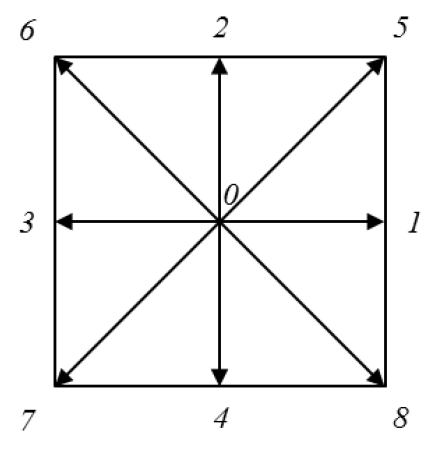
\includegraphics[width=0.35\textwidth]{figures/d2q9.png}} \qquad
	\subfloat[D3Q19]{\label{fig:d3q19}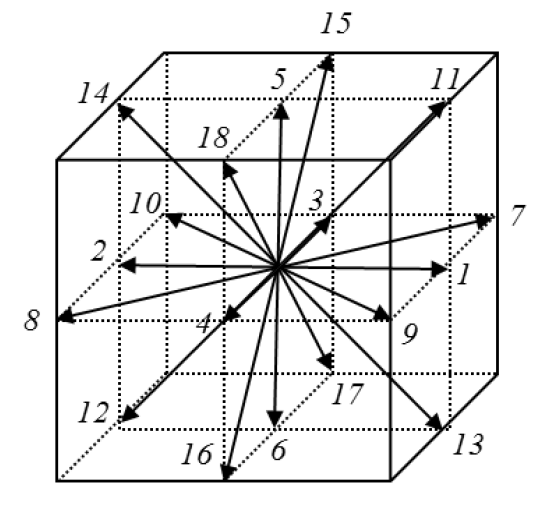
\includegraphics[width=0.38\textwidth]{figures/d3q19.png}} 
	\caption{D2Q9模型和D3Q19模型速度离散示意图}
	\label{fig:dnqm}
\end{figure}

\noindent D2Q9模型适用于二维流动问题,将速度根据大小和方向的不同分为了9类;
D3Q19模型适用于三维流动问题,速度离散也更加复杂,将速度根据大小和方向的不同分为了19类。

LBM方法相对于宏观方法具有精度高的特点,与传统方法相比,对流项(碰撞项)是线性的,算法简单;由于粒子的运动只有碰撞和迁移,LBM方法编程容易;
此外,LBM运算具有局部性,每个粒子只与周围相邻粒子有关,局部运算可同步进行,适合并行计算。
因为以上优点,LBM方法在CFD领域应用广泛,利用深度学习技术提升LBM方法的模拟效率具有重要意义。


\subsection{雷诺平均N-S(RANS)方程}
流体流动一般由以下三个基本定律来控制:
(1)质量守恒定律;(2)牛顿第二定律;(3)能量守恒定律。基于这三个基本的物理学定理构建的流动模型,将导出一组控制方程,比如适合粘性流动的Navier-Stokes方程(N-S方程)。

流体流动有不同的流动状态,当流速很小时,流体分层流动,互不混合,称为层流;当流速逐渐增大,流体的流线开始出现波浪状的摆动,摆动的频率及振幅随流速的增加而增加,此种流况称为过渡流;当流速增加到很大时,流线不再清楚可辨,流场中有许多小漩涡,层流被破坏,相邻流层间出现滑动和混合,这时的流体作不规则运动,这种运动称为湍流。

湍流运动过程十分复杂,在数学上表现出极高的非线性,使用数值模拟方法解决湍流一直是流体力学研究的难点。
虽然N-S方程能够准确地描述湍流运动的细节,但求解这样一个复杂的方程会花费大量的精力和时间。

目前在CFD领域,解决湍流问题的方法主要包括直接数值模拟(Direct numerical simulation,
DNS)、大涡模拟(Large eddy simulation,LES)和雷诺平均( Reynold average Navier-Stokes,RANS)。
其中DNS和LES对网格精细度要求较高,在工程应用上还处于尚不成熟的阶段。
为了在精度和效率上满足实际工程需要,研究者提出了基于时均理论的雷诺平均N-S模型,RANS在工程上应用也最多。
对于本文研究的稳态不可压流动,在笛卡尔坐标系下有,连续性方程:

\begin{equation}
\label{连续性方程}
\frac{\partial \rho}{\partial t}+\frac{\partial(\rho u)}{\partial x}+\frac{\partial(\rho v)}{\partial y}+\frac{\partial(\rho w)}{\partial z}=0\end{equation}

\noindent 对动量方程采用二阶迎风对流格式离散:


\begin{equation}\begin{array}{c}
\label{动量方程}
u \frac{\partial u}{\partial x}+v \frac{\partial u}{\partial y}+w \frac{\partial u}{\partial z}=-\frac{1}{\rho} \frac{\partial p}{\partial x}+\frac{\mu}{\rho} \nabla^{2} u \\
u \frac{\partial v}{\partial x}+v \frac{\partial v}{\partial y}+w \frac{\partial v}{\partial z}=-\frac{1}{\rho} \frac{\partial p}{\partial y}+\frac{\mu}{\rho} \nabla^{2} v \\
u \frac{\partial v}{\partial x}+v \frac{\partial w}{\partial y}+w \frac{\partial w}{\partial z}=-\frac{1}{\rho} \frac{\partial p}{\partial z}+\frac{\mu}{\rho} \nabla^{2} w
\end{array}
\end{equation}


\noindent 对方程\ref{连续性方程}和\ref{动量方程}进行雷诺平均有:
\begin{equation}\frac{\partial \rho}{\partial t}+\frac{\partial}{\partial x_{i}}\left(\rho \bar{u}_{i}\right)=0\end{equation}

\begin{equation}\frac{\partial}{\partial t}\left(\rho \bar{u}_{i}\right)+\frac{\partial}{\partial x_{i}}\left(\rho \bar{u}_{j} \bar{u}_{i}\right)=-\frac{\partial \bar{p}}{\partial x_{i}}+\frac{\partial \bar{\sigma}_{i j}}{\partial x_{j}}+\frac{\partial}{\partial x_{j}}\left(-\rho \bar{u}_{i}^{\prime} \bar{u}_{j}^{\prime}\right)\end{equation}

\noindent 其中$\bar{u}_{i}$为雷诺平均速度分量,$\rho$为密度,$p$为压强,$\bar{u}_{i}^{\prime}$平均脉动速度,$\partial \bar{\sigma}_{i j}$为应力张量分量。


一般地,在对湍流流动的N-S方程平均后,得到的平均方程中会包含未知的雷诺应力项,导致了方程求解的不封闭问题。
因此需要根据湍流运动规律以寻找附加条件和关系式构建湍流模型使方程封闭。
此外,在进行雷诺平均的过程中损失了部分流动细节,引入湍流模型对于找回这些细节十分必要。
对于RANS湍流模拟,根据Boussinesq\cite{schmitt2007boussinesq}假设,粘性系数由层流部分和湍流部分构成,
即$\nu=\nu_{L}+\nu_{T}$,其中$\nu_{L}$是层流运动粘性系数(laminar kinematic viscosity), $\nu_{T}$是湍流运动粘性系数(eddy-viscosity variable),由湍流模型方程计算得到。

常用的湍流模型可根据所采用的微分方程数进行分类为:零方程模型、一方程模型、两方程模型、四方程模型、七方程模型等\cite{1998A}。本文使用的湍流模型是Spalart-Allmaras(SA)模型\cite{SAequation},
是一种主要用在航空领域的单方程湍流模型,对墙壁束缚(wall-bounded)流动,显示出很好的效果。
SA模型认为在自由剪切流中能量和信息由大尺度流动流向小尺度流动,涡粘系数只有产生项和扩散项,所以满足以下基本运输方程:

\begin{equation}
\begin{split}
\frac{D F}{D t}= & \frac{\partial F}{\partial t}+(u \cdot \nabla) F \\ = & {Diffusion} + {Production} - {Destruction}
\end{split}
\end{equation}

\noindent 其中$F$外力,\textit{diffusion}是扩散项,\textit{production}是产生项,\textit{destruction}是损失项。
对于湍流运动粘性系数$\nu_{T}$应用该运输方程有:

\begin{equation}\label{SA_equo}
\begin{split}
\frac{D \nu_{T}}{D t}=& \frac{1}{\sigma}\left[\nabla \cdot((\nu_{L}+\nu_{T}) \nabla \nu_{T})+c_{b 2}(\nabla \nu_{T})^{2}\right] +c_{b 1} \tilde{S} \nu_{T} - \\ &c_{w 1} f_{w}\left[\frac{\nu_{T}}{d}\right]^{2}
\end{split}
\end{equation}

\noindent 其中$\sigma$普朗特数,$c_{b 1}$和$c_{b 2}$为闭合常数,$d$表示到壁面的最短距离。
$\tilde{S}$可以通过$d$和速度$u$计算得到,
$f_{w}$是一个关于$\tilde{S}$和$\nu_{T}$无量纲函数,用于解决在边界层外部损失项收敛慢的问题。

虽然许多湍流模型在某些特定的应用场景取得成功,但至今仍未有一个有效的通用的湍流模型,这也直接导致了RANS缺少普适性。
本文首先基于特定流场条件,模拟生成流场数据集,然后利用深度学习方法从大量流场数据学习流场运动规律,
最后得到能够进行快速精准流场预测的代替模型。


\section{深度学习相关模型介绍}
深度学习是机器学习的重要分支,自2006年提出以来,深度学习理论和技术以及获得了长足的发展,常见的深度学习模型有深度信念网络\cite{深度信念网络},自动编码器\cite{Bengio2013Representation},卷积神经网络\cite{Lecun1998Gradient},递归神经网络\cite{Williams2014A},生成对抗网络\cite{GAN}等。
此外,深度学习在与强化学习、图网络结合方面也非常成功,比较前沿的研究领域有深度强化学习\cite{Deepreinforcementlearning}和图神经网络\cite{2016Semi}等。
深度学习的快速发展为解决气动优化提供了新的思路和方法,
利用深度学习方法提升气动优化效率的核心思想是基于神经网络构建从输入到输出的映射函数,
从而代替或者加速CFD求解器的迭代计算过程,
不同于常规的图像分类任务,深度神经网络需要在大量数据中学习到从给定输入到对应输出的表示方法。

针对流场数据中的欧式空间数据,经过类比分析,我们发现图像处理中的image-to-image\cite{DBLP:conf/miccai/RonnebergerFB15,DBLP:conf/cvpr/LongSD15,isola2017image,CycleGAN2017,DBLP:conf/cvpr/AmodioK19}的转换方法尤其适用于气动优化场景。
对于非欧式空间数据,本文引入了基于图神经网络的架构进行模型训练。
如何将流场数据处理成为深度神经网络可接受的形式将在第三章详细阐述,本节重点介绍三类用于图像回归任务的深度神经网络和图神经网络中的图卷积网络。
关于深度学习的其他基础理论知识,包括网络基础结构单元,损失函数,优化算法等,可参见文献\cite{dnnsurvey}。

\subsection{卷积自编码网络}
卷积自编码网络(Convolutional Autoencoders)是自编码网络\cite{Bengio2013Representation}的变体。
自编码网络及其变体都有类似的网络结构:编码器和解码器。
传统的自编码器是一种无监督学习算法,数据没有标签,
输入数据$X$经过编码器处理得到输入数据的特征表示z,编码结果经过解码器得到输出$X^{\prime}$,具体过程可以表示为:
\begin{equation}
z=g(X ; \phi) 
\vspace{-0.2cm}
\end{equation}
\begin{equation}
X^{\prime}=f(z ; \theta)
\end{equation}
其中$g(\bullet ; \phi)$和$f(\bullet ; \theta)$分别表示编码器和解码器,$\phi$和$\theta$是相应的参数。

损失函数一般可以定义为输入$X$和输出$X^{\prime}$的最小均方误差(Mean Squared Error,MSE):
\begin{equation}
Loss_{MSE} = \min _{\phi, \theta}\left\|X-X^{\prime}\right\|_{2}^{2}
\end{equation}

一般而言,z的维度远小于输入$X$的维度,网络通过这样编码和解码的方式,实现对输入数据的降维且尽量不损失数据信息。

但是传统的自编码器在处理图片格式数据时,由于采用了全连接操作,忽略了图像中的空间关系,数据切片和数据堆叠会导致信息大量丢失。
为了克服这一缺点,卷积自编码网络采用卷积层来构造自编码器。
图\ref{fig:CAE}是卷积自编码网络的示意图,深色部分代表编码器,通常由卷积层和池化层构成,卷积层负责信息提取,池化层负责空域下采样;
浅色部分代表解码器,由卷积层和上采样层构成,有时也利用逆卷积操作替代卷积和上采样操作进行原始信息的复原。

\begin{figure}[htp]
	\centering
	%\includegraphics[width=0.42\textwidth]{data/MLP.pdf}
	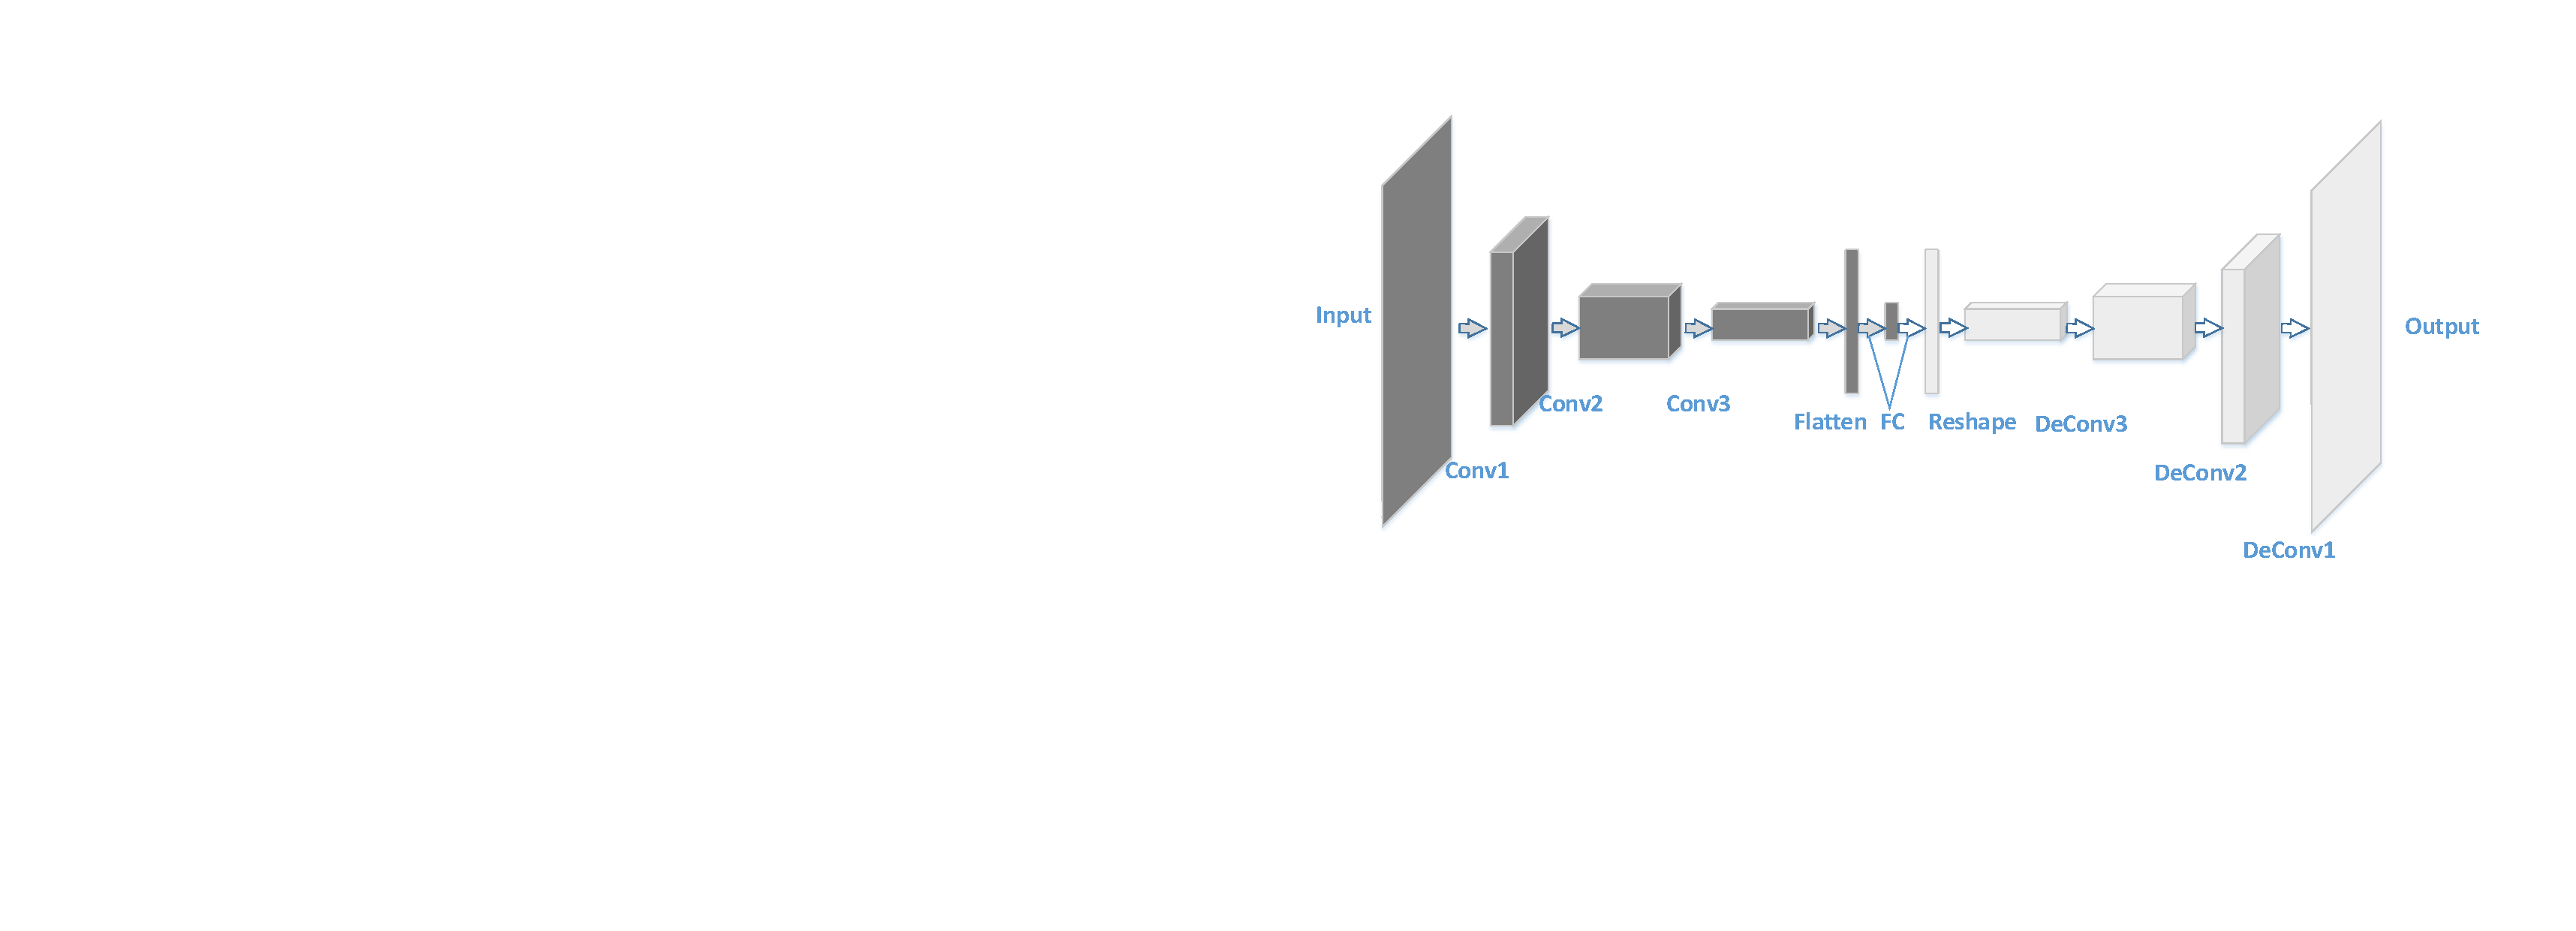
\includegraphics[width=0.92\textwidth]{figures/CAE.pdf}
	\caption{卷积自编码网络示意图}
	\label{fig:CAE}
\end{figure}

逆卷积操作原理如图\ref{fig:conv_dconv}所示,逆卷积操作可以看出是常规卷积操作的逆过程,不同点在于,为了还原原始输入的尺寸,通常需要进行填充(padding)操作(如图\ref{fig:dconv}中的空白区域)。


\begin{figure}[htb]
	\centering
	\subfloat[卷积操作]{\label{fig:conv}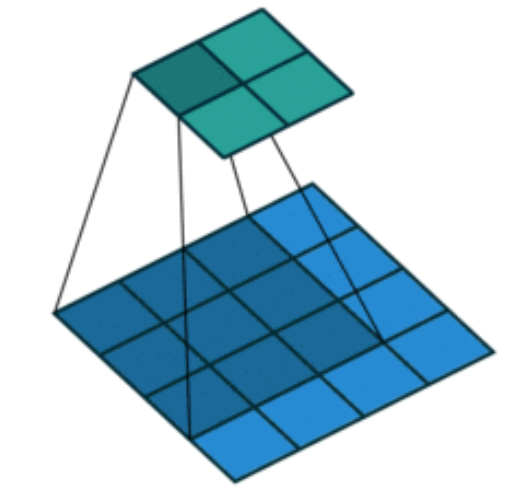
\includegraphics[width=0.42\textwidth]{figures/conv.png}} \qquad
	\subfloat[逆卷积操作]{\label{fig:dconv}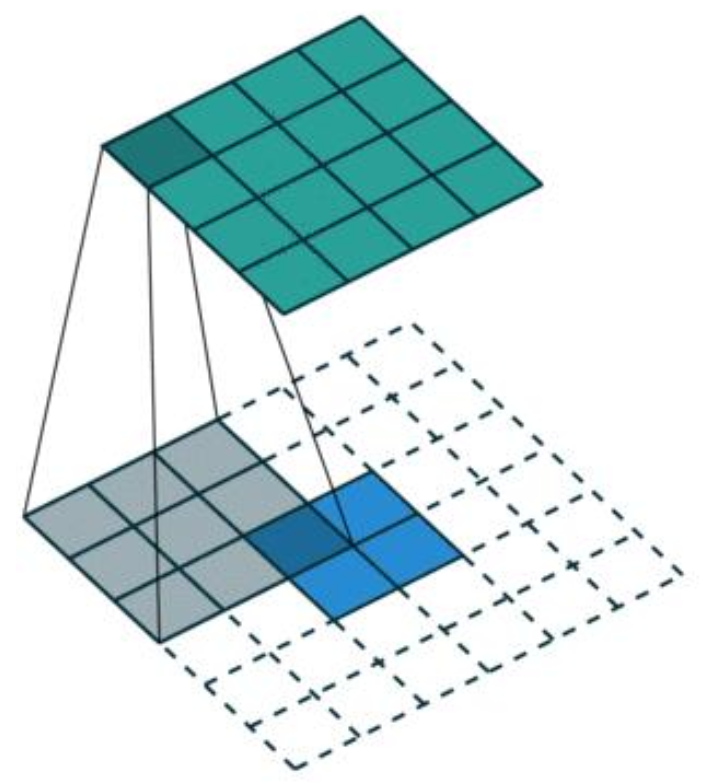
\includegraphics[width=0.38\textwidth]{figures/dconv.png}} 
	\caption{逆卷积操作原理}
	\label{fig:conv_dconv}
\end{figure}

%\begin{figure}[htp]
%	\centering
%	%\includegraphics[width=0.42\textwidth]{data/MLP.pdf}
%	subfigure[卷积操作]{\label{fig:conv}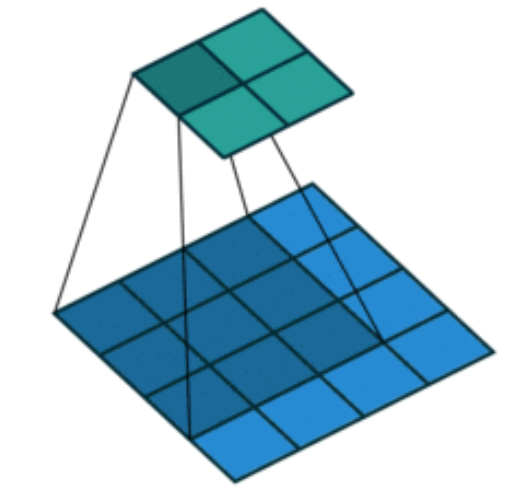
\includegraphics[width=0.42\textwidth]{figures/conv.png}}
%	subfigure[逆卷积操作]{\label{fig:dconv}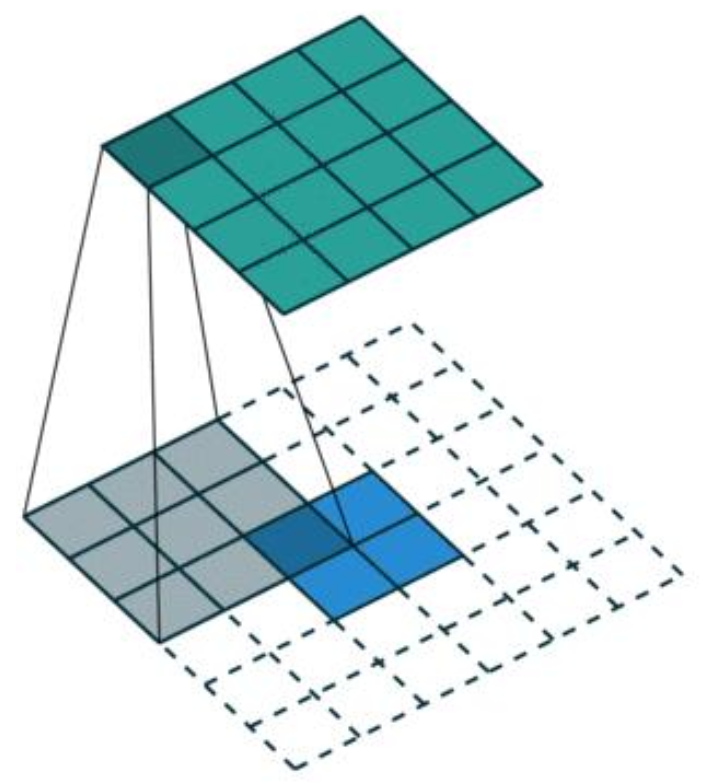
\includegraphics[width=0.42\textwidth]{figures/dconv.png}}
%	\caption{逆卷积操作原理}
%	\label{fig:conv_dconv}
%\end{figure}


对于无监督学习,在卷积神经网络的编码器和解码器的衔接处,利用全连接层,也可以提取带图像数据特征表示;在进行有监督学习时,网络更关注解码器的输出$Y^{\prime}$而不是z,损失函数转化为:
\begin{equation}
Loss_{MSE} = \min _{\phi, \theta}\left\|Y-Y^{\prime}\right\|_{2}^{2}
\end{equation}
从而可以利用卷积神经网络进行有监督学习任务,在气动流场模拟领域已有基于卷积自编码网络开展的工作\cite{DBLP:conf/kdd/GuoLI16}。



\subsection{基于深度学习的图像分割模型}
图像分割一直是计算机视觉领域的难题,也是该领域的研究热点。
所谓图像分割是指根据灰度、彩色、空间纹理、几何形状等特征把图像划分成若干个互不相交的区域,使得这些特征在同一区域内表现出一致性或相似性,而在不同区域间表现出明显的不同。
传统的方法有基于阈值的分割方法;基于区域的图像分割方法;基于边缘检测的分割方法;基于小波分析和小波变换的分割方法;基于遗传算法的分割方法等\cite{图像分割方法综述}。

近年来,深度学习方法开始应用到图像分割,通过搭建神经网络,对训练样本进行有监督学习,得到图形分割的模型。根据分割应用任务不同,图像分割分可分为普通分割、语义分割和实例分割。其中:普通分割是指对分属不同区域的像素点进行分类;语义分割是在分类的基础上识别出每一块区域的语义;实例分割在在语义分割的基础上,进一步对每个识别目标进行编号。本节重点介两种经典的语义分割网络:全卷积网络和U-net网络,分别适用于自然图像分割和医疗图像分割。


\subsubsection{全卷积网络}
2015年Long等人提出的全卷积网络(Fully Convolutional Networks,FCN)用于图像语义分割\cite{Long2015Fully}。自从提出后,FCN已经成为语义分割的基本框架,后续算法都借鉴了该框架的思想。

\begin{figure}[htp]
	\centering
	%\includegraphics[width=0.42\textwidth]{data/MLP.pdf}
	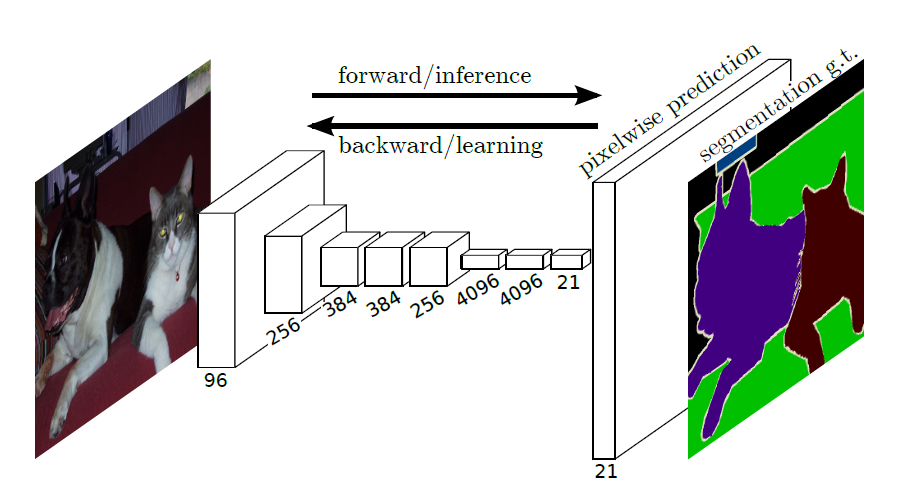
\includegraphics[width=0.88\textwidth]{figures/FCN.png}
	\caption{FCN网络结构图}
	\label{fig:FCN}
\end{figure}

如图\ref{fig:FCN}所示,FCN参考了图像分类网络中的VGG16\cite{2014Very}网络架构。图像分类网络只能对整个图片进行分类而不能识别每个像素点的类别。
为了实现逐像素分类的目的,FCN用卷积层替换了VGG网络中的全连接层,最后利用逆卷积的上采样方法将特征图恢复成原始图片大小,从对整张图片的稀疏分类转换成对每个像素点进行密集分类(dense prediction),达到图像分割的目的。

FCN的另一个特点是利用了全局信息和局部信息。经过多次卷积和池化操作以后,得到的图像越来越小,分辨率越来越低,最后产生了高维特征图。如果直接对进行上采样至原始图片大小,会产生模糊的分割结果。为了解决这一问题,FCN使用了如图\ref{fig:FCN_skip}所示的skip layer的方法。

对于FCN-32s,高层得到的粗糙层(conv7)进行32倍上采样操作,再对每个点进行softmax逻辑回归处理,得到每一个像素点的分类。

对于FCN-16s,先将conv7的结果进行2倍上采样,再将上采样结果与浅层的精细层(pool4)进行逐点相加,最后进行16倍的上采样操作得到与原始输入尺寸相同的图像分割结果。

对于FCN-8s,先将conv7的结果进行4倍上采样,将pool4的结果进行2倍上采样,再将上采样结果与更浅层的精细层(pool3)进行逐点相加,最后进行8倍上采样操作和softmax处理。

通过skip layer的方法,融合多层特征图,有效整合了粗粒度的语义信息和细粒度的位置信息,有利于提高分割准确性。
尽管8倍上采样的FCN的分割效果已经有了很大提升,但是结果还是比较模糊,对分割区域边界不敏感;此外,对每个像素点单独进行分类,没有充分考虑图像的空间上的联系。

\begin{figure}[htp]
	\centering
	%\includegraphics[width=0.42\textwidth]{data/MLP.pdf}
	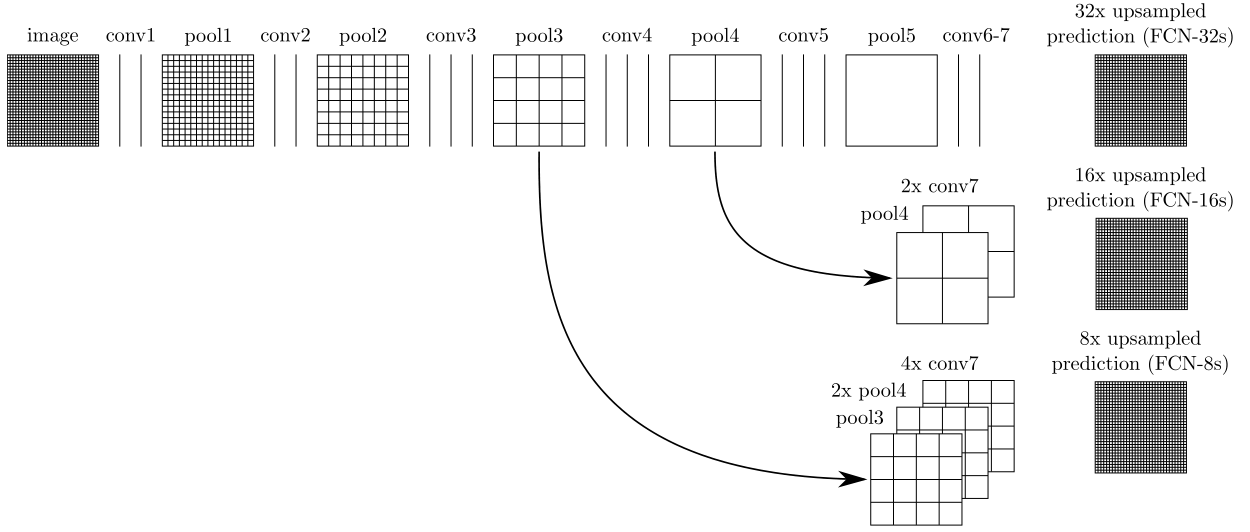
\includegraphics[width=0.88\textwidth]{figures/FCN_skip.png}
	\caption{FCN采用的skip layer方法}
	\label{fig:FCN_skip}
\end{figure}

\subsubsection{U-net网络}
2015年,Ronneberger等人\cite{DBLP:conf/miccai/RonnebergerFB15}提出了U-net网络结构,U-net是基于FCN的一种语义分割网络,适用于做医学图像的分割。U-net修改并扩展了FCN网络结构,使它在使用少量的数据进行训练的情况下获得精确的分割结果。
其主要思想是在下采样网络的后面补充一个对称的上采样网络,多个上采样层增加了网络的参数和表示能力,有利于提升输出结果的分辨率。
对称的网络结构形似英文字母“U”,所以被称为U-net。

U-net网络结构如图\ref{fig:unet}所示:
蓝/白色框表示特征图;蓝色箭头表示3x3卷积层,用于特征提取;灰色箭头表示 skip-connection,用于特征融合;红色箭头表示池化层,用于降低维度;绿色箭头表示上采样 upsample,用于恢复维度;青色箭头表示1x1卷积,用于输出结果。其中灰色箭头中的copy就是atenate操作,将深层的特征图和浅层的特征图在通道方向拼接;crop是为了让两者的长宽一致,保证拼接后的特征图大小一致。


\begin{figure}[htp]
	\centering
	%\includegraphics[width=0.42\textwidth]{data/MLP.pdf}
	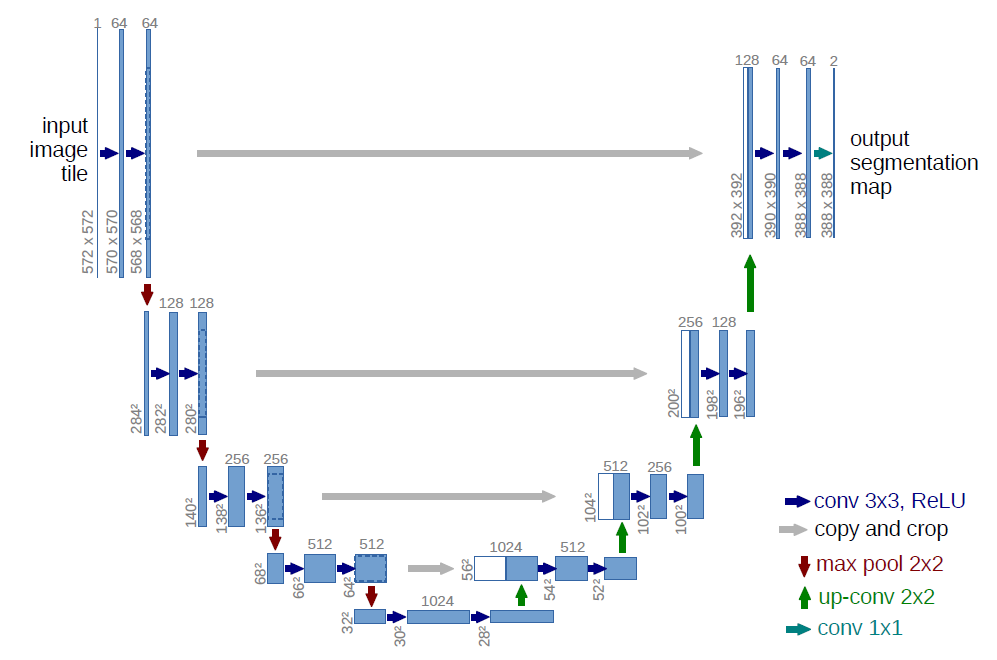
\includegraphics[width=0.88\textwidth]{figures/unet.png}
	\caption{U-net网络结构图\cite{DBLP:conf/miccai/RonnebergerFB15}}
	\label{fig:unet}
\end{figure}

U-net主体结构包括一个捕获上下文信息的收缩路径和一个允许精确定位的对称拓展路径:
收缩部分和扩展部分都有4个采样层。这种架构延续了Encoder-Decoder的思想。
Encoder由卷积操作和下采样操作组成,文中所用的卷积结构统一为3x3的卷积核,填充为 0,步长为1;Decoder部分采用的上采样的方式与FCN中的反卷积不同,为双线性插值。
此外,为了更好融合位置信息和语义信息,U-net拓展了FCN中skip layer的思想,在“U”形网络的对称部分添加了skip connection。与FCN的加操作不同,U-net使用了叠操作(concatenation)增加了特征的厚度,保留了更多浅层的位置信息,这使得上采样层可以在浅层特征与深层特征在训练时进行自适应选择,这对语义分割任务来说更有优势。

由于在医疗图像分割上取得巨大成功,许多研究者针对不同的图像分割任务对U-net进行了改进,产生了许多U-net变体包括V-Net\cite{2016V}、UNet++\cite{unet++}、U-NetPlus\cite{unetplus}和3D U2-Net\cite{20193D}等,提升了模型的推理速度和精度。


\subsection{Pix2Pix网络模型}
对于气动流场预测,核心问题是实现从输入到输出的映射。
除了前文提到的自编码网络和图像分割网络,基于生成对抗网络(Generative Adversarial Network, GAN)的图像风格迁移模型也在解决像素到像素的映射问题上展示出的强大潜力。
GAN在图像生成、风格迁移、超分辨重建等领域已经得到了广泛的应用,
本节我们重点介绍Pix2Pix网络模型\cite{isola2017image}。

Pix2Pix网络基于条件生成对抗网络(Conditional Generative Adversarial Network, cGAN)\cite{cGAN},通过添加条件约束信息来指导完成图像转换任务,比如从标签图合成相片,从线稿图重构对象,给图片上色等。
和传统的GAN网络类似,在Pix2Pix模型训练过程中,迭代地训练生成器和判别器,生成器尽可能生成接近真实的样本,企图“欺骗”判别器;判别器尽可能识别出真实的样本和生成的样本,获得更高的得分。这样的对抗训练过程类似博弈游戏,随着训练的进行,生成器和判别器的能力不断提升直到达到令人满意的效果。
由于添加了约束条件,Pix2Pix网络的输入不再是普通GAN网络中的随机变量,其网络结构示意图
如图\ref{fig:cgan}所示:

\begin{figure}[htp]
	\centering
	%\includegraphics[width=0.42\textwidth]{data/MLP.pdf}
	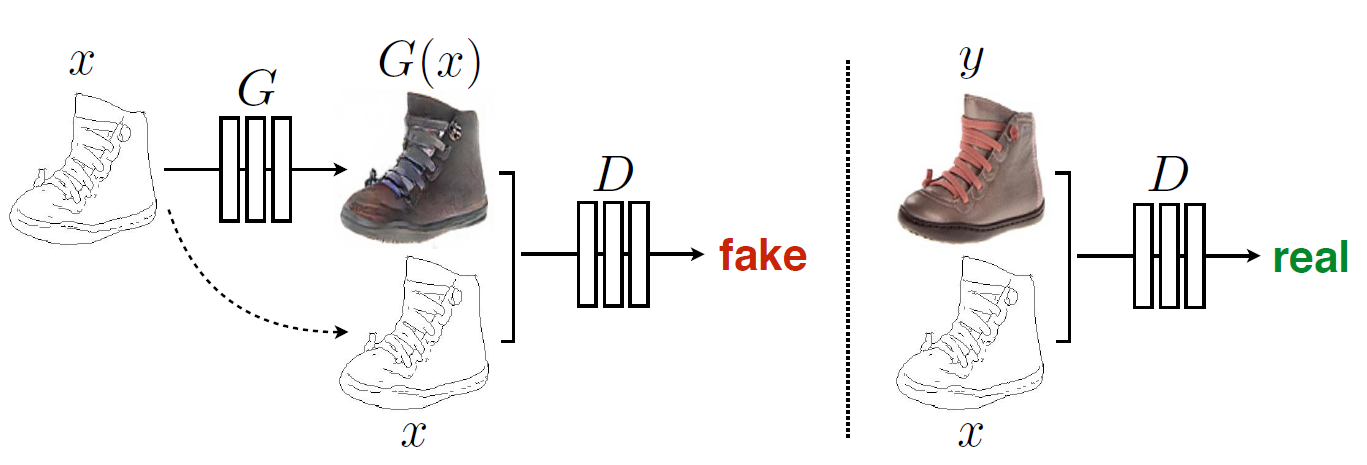
\includegraphics[width=0.88\textwidth]{figures/cGAN.png}
	\caption{Pix2Pix网络结构示意图}
	\label{fig:cgan}
\end{figure}

其中x是条件输入,y是对应的标签,每个输入x唯一对应一个标签y。
在训练生成器时,x进过生成器$G$得到生成图像$G(x)$;
在训练判别器时,输入x和对应生成图像$G(x)$或标签y通过通道维度的叠操作进行拼接,一同送入判别器,判别器会输出概率值,表示是否为一对真实样本。



Pix2Pix网络利用类似U-net的结构代替自编码网络作为生成器,
在输入和输出之间存在很多可以共享的低级信息,采用skip-connection的结构有利于传递这些底层信息和重构图像。
对于判别器网络,Pix2Pix提出了PatchGAN架构。
传统GAN判别器通常对生成样本整体进行判断,对于图片而言,直接输出整张图片是真实样本的概率。而图像转换任务中关注像素到像素的转换效果,所以在这里提出了分块判断的算法,在图像的每个块上去判断是否为真,输出平均预测结果。


条件GAN采用的损失函数通常为:
\begin{equation}
\begin{aligned}
\mathcal{L}_{c G A N}(G, D)= &\mathbb{E}_{x,y}[\log D(x,y)]+\\
&\mathbb{E}_{x,z }[\log (1-D(x, G(x,z))]
\end{aligned}
\end{equation}

\begin{equation}
\begin{aligned}
\mathcal{L}_{c G A N}(G)= \mathbb{E}_{x,z}[\log (1-D(x, G(x, z))]
\end{aligned}
\end{equation}

\noindent 其中z为输入随机变量,在Pix2Pix网络输入仅为x。
此外,为了保证像素级低频信息的预测精度,Pix2Pix网络的损失函数还引入了$L_1$损失项:

\begin{equation}
\begin{aligned}
\mathcal{L}_{L 1}(G)=\mathbb{E}_{x_1, x_2, y}\left[\|y-G(x_1, x_2)\|_{1}\right]
\end{aligned}
\end{equation}

考虑到训练的最终目标是获得一个性能良好的生成器,同时生成器和判别器进行着对抗的训练,所以训练的最终目标是:
\begin{equation}
\begin{aligned}
G^{*}=\arg \min _{G} \max _{D} \mathcal{L}_{c G A N}(G, D)+\lambda \mathcal{L}_{L 1}(G)
\end{aligned}
\end{equation}
\noindent 其中$\lambda$是$L_1$损失函数项的权重系数。


\subsection{图卷积神经网络}

在深度学习发展过程中,卷积神经网络(Convolutional Neural Network, CNN)和循环神经网络(Recurrent Neural Network, RNN)在图像识别、语义分割、自然语言处理等领域发挥了重要作用。
无论是图像还是语言,在CNN或RNN进行处理时都被转换成结构规则的数据形式,都属于欧式空间的数据。
然而现实生活中有很多不规则的数据结构,如社交网络、化学分子结构、生物网络等;即使是语言,其内部实际是复杂的树形结构,
只是RNN将其处理成向量的形式便于神经网络训练。
图结构通常被用来表示这些非欧式空间的数据,但是在图结构中,每个节点周围的结构千差万别,不同于图像和向量化的语言数据具有平移不变性,因此不可能直接利用CNN或RNN进行处理。

近年来,人们对深度学习方法在图上的拓展进行了大量的研究,研究人员借鉴CNN、RNN以及图嵌入技术的思想,
定义和设计了专用于处理图结构数据的神经网络,即图神经网络(Graph  Neural  Network, GNN)。
文献\cite{2019A}将GNN分为五大类:图卷积网络(Graph Convolution Networks,GCN)、 图注意力网络(Graph Attention Networks)、图自编码器( Graph Autoencoders)、图生成网络( Graph Generative Networks) 和图时空网络(Graph Spatial-temporal Networks)。
本节重点介绍图卷积神经网络。

GCN方法主要分为两大类,基于谱(spectral-based)和基于空间(spatial-based)。
基于谱的方法将空域信号利用傅里叶变换转换到频域进行分析处理,完成在空域无法完成的操作。
对于无向图有正则化拉普拉斯矩阵:

\begin{equation}
\mathbf{L}=\mathbf{I}_{\mathbf{n}}-\mathbf{D}^{-\frac{1}{2}} \mathbf{A} \mathbf{D}^{-\frac{1}{2}}
\end{equation}

\noindent $I_n$为单位矩阵,A为图的邻接矩阵,D为对角矩阵。
对L进行特征值分解有:

\begin{equation}
\mathbf{L}=\mathbf{U} \mathbf{\Lambda} \mathbf{U}^{T}
\end{equation}

\noindent U是特征向量构成的矩阵,$\Lambda$是对角矩阵,对角线上的值为L的特征值。
对输入图信号x的傅里叶变换和傅里叶逆变换分别被定义为

\begin{equation}
\mathfrak{F}(\mathrm{x})=\mathbf{U}^{T} \mathrm{x} 
\end{equation}
\begin{equation}
\mathfrak{F}^{-1}(\hat{\mathrm{x}})=\mathbf{U} \hat{\mathrm{x}}
\end{equation}

\noindent $\hat{\mathrm{x}}$为傅里叶变换的结果。
定义对输入图信号的图卷积操作为:

\begin{equation}
\begin{aligned}
\mathrm{x} *_{G} \mathrm{g} &=\mathfrak{F}^{-1}(\mathfrak{F}(\mathrm{x}) \odot \mathfrak{F}(\mathrm{g})) \\
&=\mathbf{U}\left(\mathbf{U}^{T} \mathrm{x} \odot \mathbf{U}^{T} \mathrm{g}\right)
\end{aligned}
\end{equation}
\noindent 其中g是定义的滤波器,$\odot$表示哈达玛积运算。
基于频谱的图卷积网络都遵循这样的模式,它们之间关键的不同点在于选择的滤波器不同
基于谱的方法从图信号处理的角度引入滤波器来定义图卷积,根据图谱理论和卷积定理,将数据由空域转换到谱域做处理,理论基础坚实。
基于空间的方法将图卷积表示为从邻域聚合特征信息,直接在图空间上定义卷积操作,灵活性更强。




\begin{figure}[htp]
	\centering
	%\includegraphics[width=0.42\textwidth]{data/MLP.pdf}
	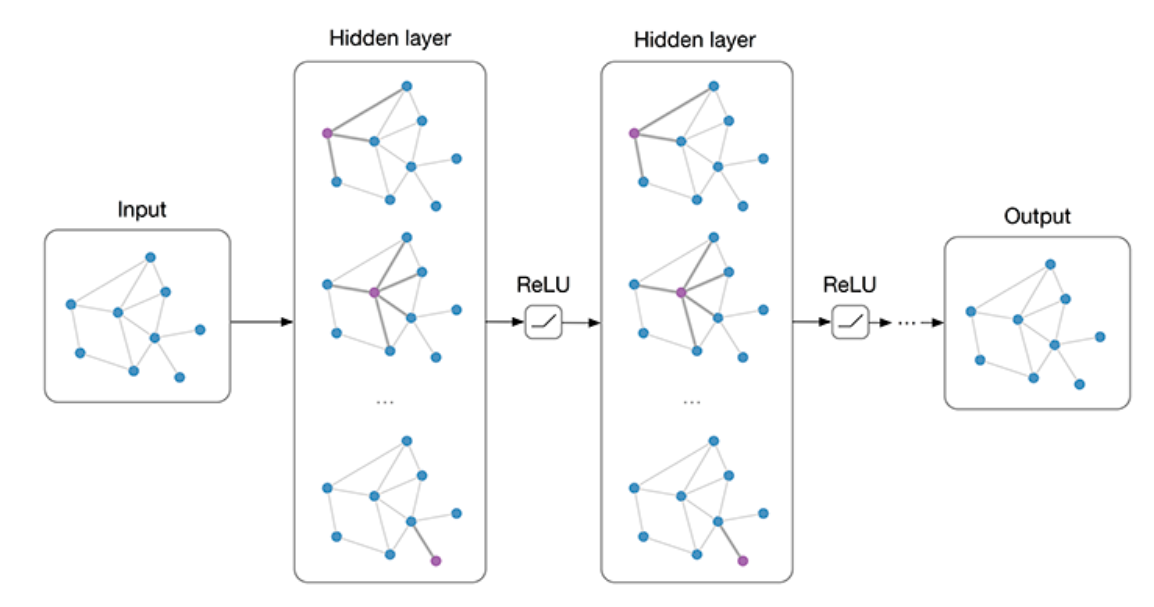
\includegraphics[width=0.88\textwidth]{figures/GCN.png}
	\caption{多层GCN网络示意图}
	\label{fig:gcn}
\end{figure}

对于图卷积算法的实现主要包括三个步骤:
\romannumeral1)发送:每一个节点将自身的特征信息经过变换后发送给邻居节点。这一步是在对节点的特征信息进行抽取变换;
\romannumeral2)接收:每个节点将邻居节点的特征信息聚集起来。这一步是在对节点的局部结构信息进行融合;
\romannumeral3)变换:把前面的信息聚集之后做非线性变换,增加模型的表达能力。
图\ref{fig:gcn}展示了一个简单的GCN网络,从图中可以发现数据的拓扑结构在训练过程中始终保持不变,
可以在训练中重复利用。
每一层的节点特征维度是不固定的,可以根据训练任务的复杂程度进行灵活的调整。

概括而言,图卷积算子的作用就是将每个节点的特征与其邻居节点的特征加权平均后传播到下一层,具有以下特点:
1)局部参数共享,计算节点特征值时,按一定规律将参与聚合的节点分为若干个子集,
同一个子集内的节点采用相同的权重;
2)节点感受域正比于层数,每一层图卷积运算只能和相邻的节点进行特征聚合;通过增加GCN层数,每个节点上参与运算的其他节点信息就更多;
3)适用于任意拓扑结构的节点与图,能同时对节点特征信息与图结构信息进行端对端学习。


%\section{实验算例介绍}
%\subsection{2D不可压层流固体外部流场}
%\subsection{2D不可压有粘翼型外部流场}



\section{本章小结}

本章首先通过对比传统CFD求解器和基于深度学习的气动优化模型的工作流程,明确了利用深度学习技术和方法要解决的CFD问题。
然后介绍了CFD相关理论知识,重点介绍了在宏观和介观层面对流体运动规律的描述。
最后分析了气动流场模拟任务和深度学习中图像回归预测任务的相似性,介绍了与本文研究内容紧密相关的深度网络模型。






\chapter{基于深度卷积网络的流场预测方法}

本章介绍了基于深度神经网络的气动流场预测方法,首先将流场数据通过合适的方法表示为深度神经网络可以接受的输入。
然后借鉴图像分割领域中的U-net网络设计了气动流场预测网络\textsc{FlowDNN},
根据气动流场预测的实际需要,通过嵌入注意力模块网络架构对\textsc{FlowDNN}进行了改进,设计了遵循守恒定律的物理损失函数。
最后利用基于LBM的求解器生成实验数据集,定义了新的预测模型评测指标并与三种基线网络进行了全面的比较。


\section{引言}

\subsection{动机分析}

为了解决传统CFD方法进行流场模拟时间、经济成本较高的问题,
本文尝试利用数据驱动的深度卷积网络实现端到端流场预测,提升气动流场模拟的效率。
基于深度卷积网络的气动特性和气动性能预测具有以下优势:
1)深度卷积网络不需要对输入特征进行人工筛选和精简,可极大地减少设计变量数目限制,
设计者能对几何外形的坐标点进行直接控制,设计变量可以细化为几何外形所有离散点的空间坐标,实现精细的外形优化。
2)深度卷积网络可以得到更加符合物理直觉的模型。如对几何外形坐标点和气动性能的关系进行建模,
输入数据是一个二阶或三阶张量,很好地保留了坐标点间的空间相邻关系,其特征提取过程具有空间上的平移不变性和缩放不变性。
3)深度卷积网络由于能够提取更深层次的特征,因而拥有更强大的归纳能力,不仅可以获得气动性能预测,
还可以将流场特征(如压力分布等)作为预测输出。

当前,基于深度学习的气动评估及其在气动优化中的应用尚处于起步阶段,
多参考深度学习在其他领域应用较为成熟的方法技术,尤其是深度卷积神经网络在计算机视觉领域的研究成果,
在深度学习优化技术应用于气动优化场景方面缺少进一步的研究,深度学习还没有与空气动力学实现交叉融合。
因此,本文提出构建嵌入物理约束的深度卷积网络模型,利用深度学习优化技术增强模型流场数据特征提取能力,
使其更加适用于处理气动优化问题。


\subsection{研究思路}
流场预测任务和图像回归预测任务相似,要解决的核心问题是利用深度神经网络学习输入到输出的映射关系。
通过对图像回归预测相关方法和技术的研究,本文基于广泛用于图像分割的U-net网络实现对气动流场的快速准确预测。

在流场数据表示方面,通过合适的数据表示方法将几何体、边界条件等流场信息表示为深度卷积网络可以接受的矩阵形式。
针对流场预测任务特点,对U-net网络架构进行改进。相对于图像分割任务,流场预测任务对模型的表示能力要求更高:
在进行图像分割时,模型只需要对每个像素点进行准确的分类,即可有效区分图像的不同区域,是一种分类任务;
在进行流场预测时,流场预测模型需要预测每个格点上的流场物理量,是一种回归任务。
因此不能简单地将图像分割中的模型迁移应用到流场预测任务中,需要在网络架构上进行针对性的改进。
此外,流场数据不同于图片数据,虽然两者都具有较强的时空相关性,但是流场数据是流体流动稳定后的结果,
流场数据的形成遵循一定的物理规律,在进行深度卷积网络训练时需要合理嵌入物理约束保证预测结果的有效性。



\subsection{基于笛卡尔网格的流场数据表示}
利用深度学习技术对气动流场进行预测首先要解决的问题就是流场数据的表示问题,即如何将边界条件,物理场(如速度矢量场)等表示为神经网络可以接受的形式。
在此我们介绍两种方法符号距离函数(Signed Distance Function,SDF)和二元法(binary representation)。


\textbf{符号距离函数}~~对于二维笛卡尔图像,图像域$\Omega \subset R^{2}$上的每个笛卡尔网格点为$(i, j)$,
使用$f(i, j)$表示符号距离函数符号。对于几何图形经过的点,$f(i, j)$值为0。设边界点集合为$Z$,则有:
\begin{equation}Z=\left\{(i, j) \in R^{2}: f(i, j)=0\right\}\end{equation}

当点在几何体内部时,$f(i, j) < 0$,当点在几何体外部时,$f(i, j) > 0$,符号距离函数$D(i, j)$具体计算公式如下:

\begin{equation}
D(i, j)=\min _{\left(i^{\prime}, j^{\prime}\right) \in Z}\left|(i, j)-\left(i^{\prime}, j^{\prime}\right)\right| \operatorname{sign}(f(i, j))
\end{equation}


\begin{figure}[htp]
	\centering
	%\includegraphics[width=0.42\textwidth]{data/MLP.pdf}
	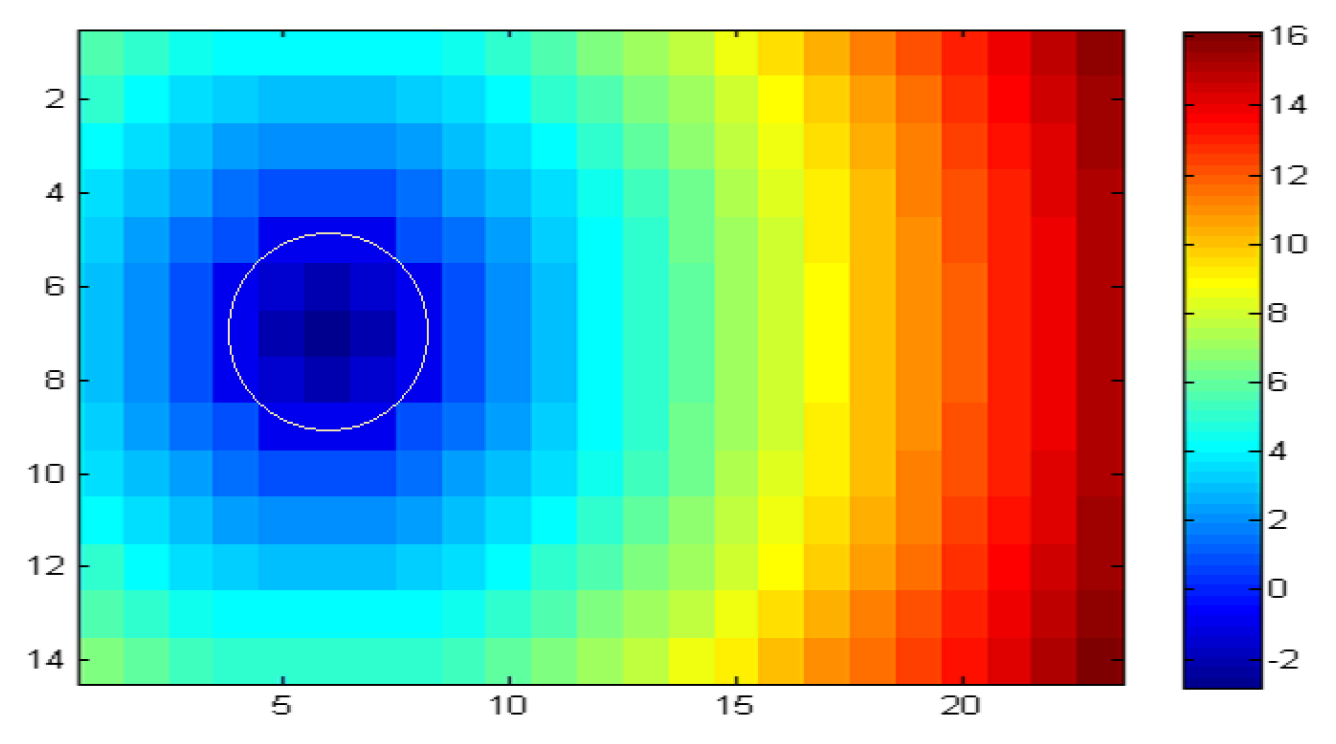
\includegraphics[width=0.54\textwidth]{figures/sdf.png}
	\caption{SDF原理示意图}
	\label{fig:sdf}
\end{figure}

$D(i, j)$表示给定点$(i, j)$到几何边界的最短距离。
图\ref{fig:sdf}是利用SDF表示二维几何图形的示意图。表示的几何图形使用白线表示,形状为圆形。


\textbf{二元法}~~图\ref{fig:binary}是二元法原理示意图,先将几何图形投射到笛卡尔网格上,使用$B(i, j)$表示二元法,则当点在几何体内部或边界时,$B(i, j) = 1$,当点在几何体外部时,$B(i, j) = 0$,通过这样表示就能将几何图形表示为一张“人工图像”。
相对于SDF,二元法进行了进一步简化,每个点到边界的物理距离没有显示的表示出来,但是对于图像数据而言,我们认为每个点的位置信息都在坐标信息中有所体现。因此,从简化预处理的角度出发,实验中使用了二元法对流场边界条件和几何图形进行表示。

\begin{figure}[htp]
	\centering
	%\includegraphics[width=0.42\textwidth]{data/MLP.pdf}
	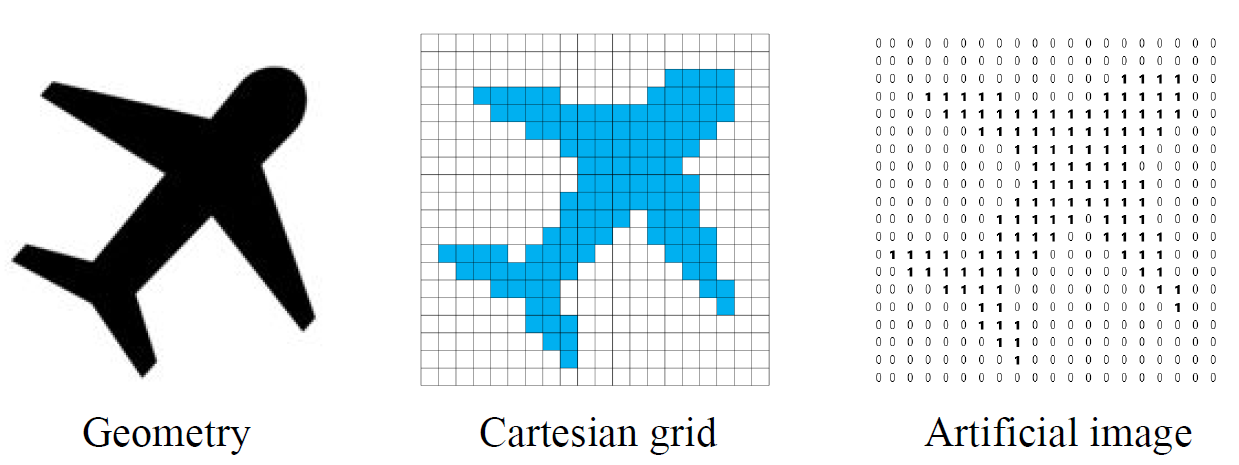
\includegraphics[width=0.64\textwidth]{figures/binary.png}
	\caption{二元法原理示意图}
	\label{fig:binary}
\end{figure}


无论是SDF和二元法,在输入流场时表示的边界条件和几何图形,在模型完成训练后进行流场预测时,每个笛卡尔网格点上的数值就不再表示几何图形,而是预测的物理量。通常输出特征图大小与输入相同,不同维度的特征图分别表示不同物理量在流场中的分布。




\section{基于U-net网络的气动流场预测}



\subsection{稳态流场预测深度模型(\textsc{FlowDNN})}
本章基于U-net网络优化设计了专用于稳态流场预测的深度神经网络架构\textsc{FlowDNN},
图\ref{fig:flowdnn}展示了\textsc{FlowDNN}网络结构。


\begin{figure}[htp]
	\centering
	%\includegraphics[width=0.42\textwidth]{data/MLP.pdf}
	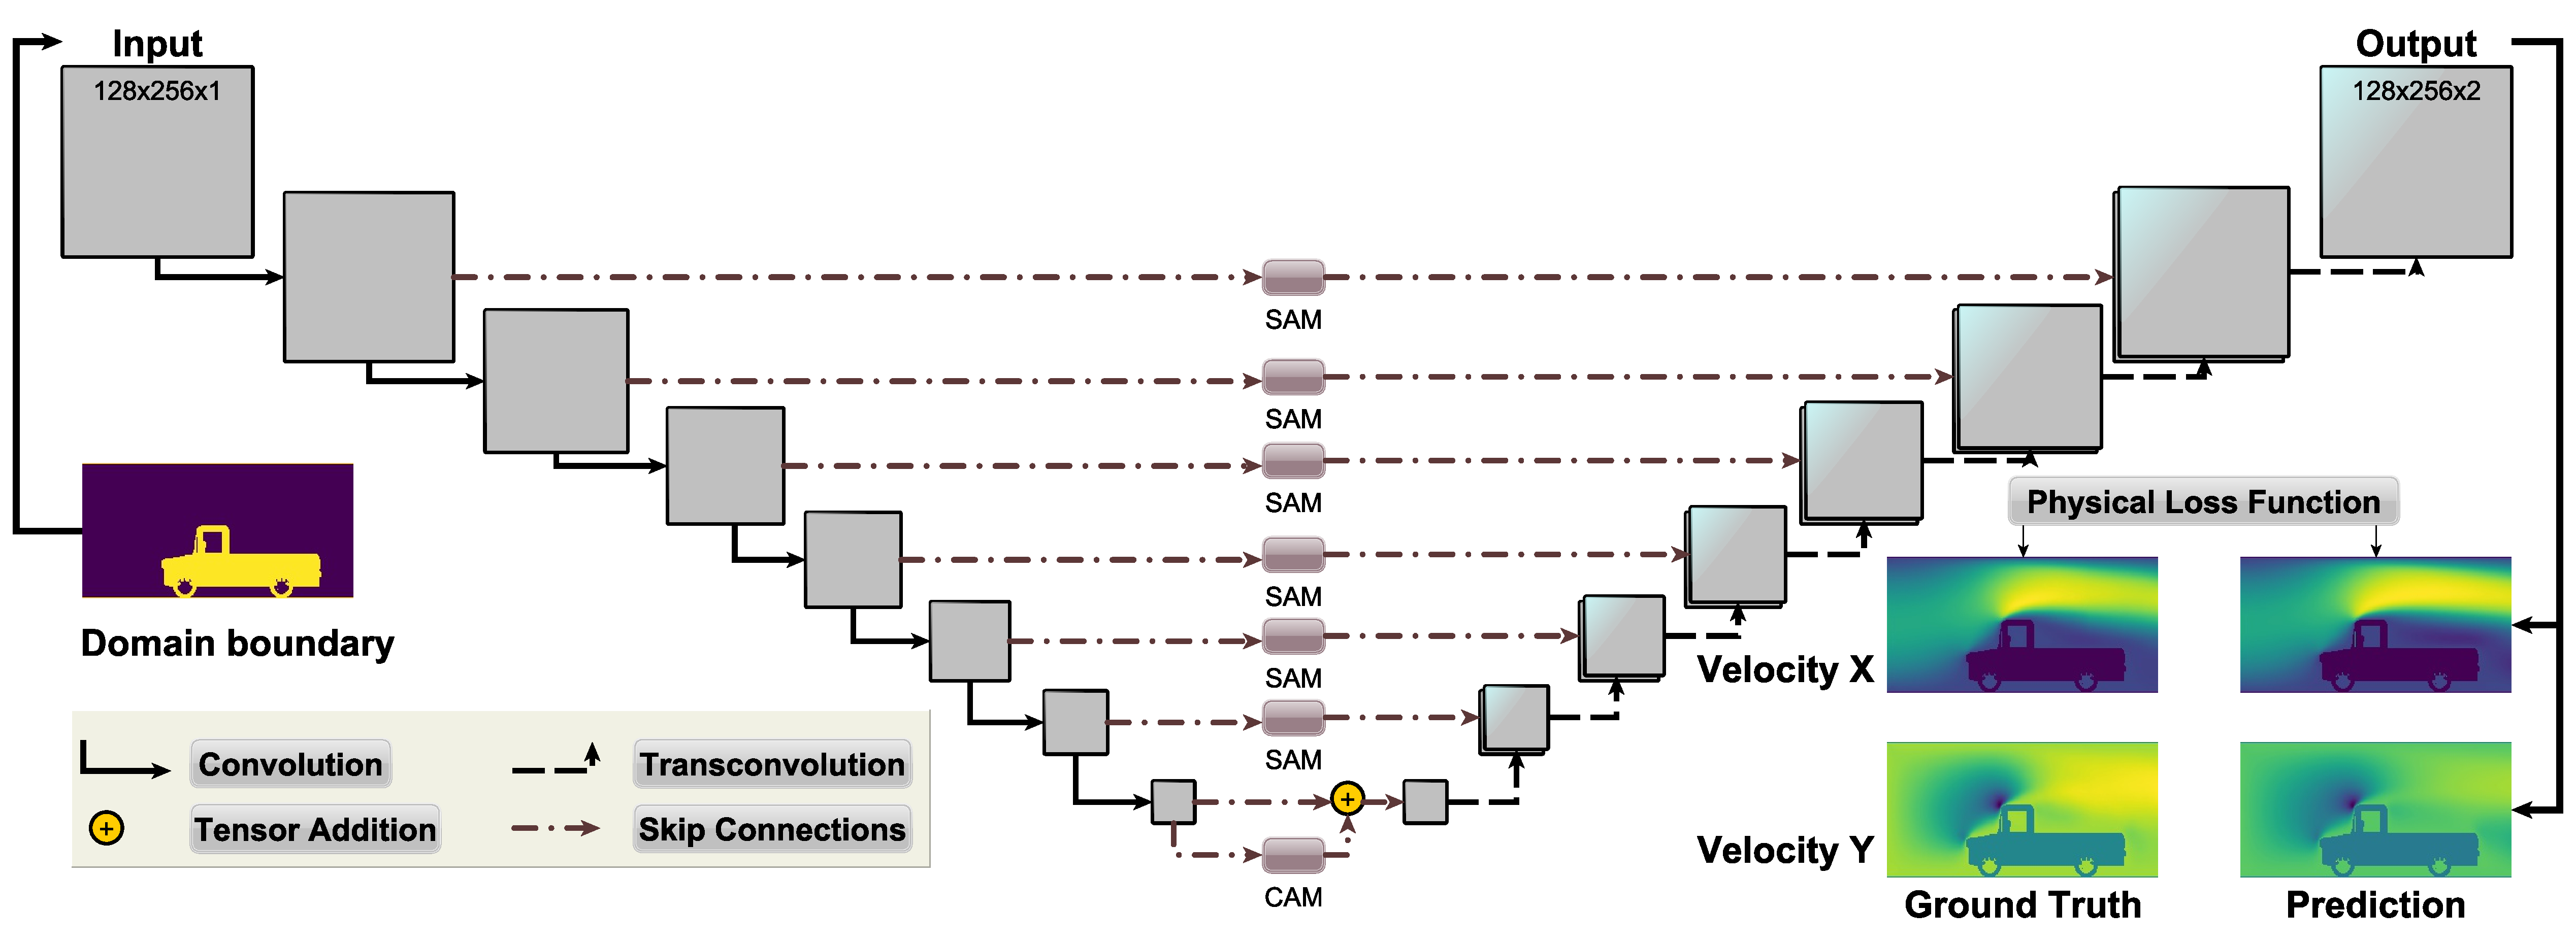
\includegraphics[width=0.99\textwidth]{figures/data/architecture.pdf}
	\caption{\textsc{FlowDNN}网络结构示意图}
	\label{fig:flowdnn}
\end{figure}

\noindent 黑色实线箭头表示卷积层和黑色虚线箭头表示反卷积层,棕色箭头表示嵌入注意力模块的skip connection。
流场边界和几何外形经过预处理得到“人工图像”作为网络输入。 输出是预测的二维速度场,
预测值和真值的损失函数为物理损失函数,用于神经网络反向传播。


\begin{table}[htp]
	\caption{
		\textsc{FlowDNN}的网络结构细节}
	\centering
	\begin{tabular}{p{3cm}p{3cm}p{3cm}p{3cm}}
		\toprule[0.4mm]
		& \multicolumn{1}{l}{编码部分} & \multicolumn{1}{l}{解码部分} \\
		\midrule
		
		\textit{Input}   & 128 x 256 x 1	& 1 x 2 x 128    \\
		\midrule
		\textit{(DE)CONV1}   &	4 x 4, 16, 2	& 2 x 2, 128, 2      	\\
		\textit{(DE)CONV2}   &	4 x 4, 32, 2	& 4 x 4, 128, 2    	\\
		\textit{(DE)CONV3}   &	4 x 4, 32, 2	& 4 x 4, 64, 2      \\
		\textit{(DE)CONV4}   &	4 x 4, 64, 2	& 4 x 4, 64, 2      \\
		\textit{(DE)CONV5}   &	4 x 4, 64, 2	& 4 x 4, 32, 2      \\
		\textit{(DE)CONV6}   &	4 x 4, 128, 2	& 4 x 4, 32, 2      \\
		\textit{(DE)CONV7}   &	2 x 2, 128, 2	& 4 x 4, 2, 2      \\

		\midrule
		\textit{Output}   & 	1 x 2 x 128		& 128 x 256 x 2      \\
		%		Ours w/ AM \& $P^2$		&\textbf{5.20\%}  & \textbf{1.99}   	& 8.50   \\
		\bottomrule[0.4mm]
	\end{tabular}
	\label{tab:flowdnn}
\end{table}

表\ref{tab:flowdnn}展示了\textsc{FlowDNN}网络结构的具体细节。
对于输入和输出而言,128 x 128 x 1表示只有1个通道且大小为128x128的特征图。
对于(逆)卷积层来说,4 x 4表示卷积核的大小,16表示卷积核的数量,2表示步长。
作为U-net的变体,\textsc{FlowDNN}也具有“U”形架构,包括7个下采样模块和7个上采样模块分别用于编码和解码。
每个下采样模块包括一个卷积层,一个激活层和一个批标准化层;卷积核的填充(padding)为1,步长为2,
用来实现下采样以提取高维抽象特征。
由于使用了逆卷积操作,可能会使预测结果出现棋盘效应\cite{odena2016deconvolution},影响预测的精度。
所以为了消除棋盘效应的影响,本文卷积核大小设置为步长2的整数倍,而不是常用的3x3或者5x5等尺寸。
前六个卷积核的感受视野为4x4,最底部的卷积核大小为2x2,因为此时输入特征图大小仅为1x2(填充之后为3x4)。
上采样层结构类似,不同的是使用逆卷积操作进行特征图的扩展,且不再使用批标准化。
每个下采样模块和上采样模块通过skip connection连接。
为了更好的融合浅层的特征,本文在skip connection上嵌入了注意力模块(细节参考\ref{注意力}节)
,增加模型的非线性和学习能力,加强不同维度信息的交互。



\subsection{物理损失函数}
将气动流场预测问题转化为图像回归预测问题后,在深度学习中常使用均方误差或均方根误差等损失函数来指导模型训练,
使预测结果在每个像素点上尽可能接近真值。
考虑到流体运动遵循一定的流动规律,仅仅依靠传统的$L_1$或$L_2$损失函数来约束神经网络训练,
可能会导致模型给出的误差较低但是不符合物理规律的预测结果。
因此,本文基于流体流动的物理规律,提出了融合物理损失项和传统$L_1$损失项的物理损失函数,
以“软”约束的方式,指导模型训练,在保证预测结果准确率的前提下,得到满足物理一致性的结果。
对于二维定常不可压流体流动问题,其宏观控制方程可以简化为:

\begin{align}
	\frac{\partial u}{\partial x}+\frac{\partial v}{\partial y}=0 
	\label{mass}\\
	\frac{\partial(u u)}{\partial x}+\frac{\partial(u v)}{\partial y}=\frac{\partial \tau_{x x}}{\partial x}+\frac{\partial \tau_{y x}}{\partial y}-\frac{\partial p}{\partial x} 
	\label{momentu1}\\
	\frac{\partial(v u)}{\partial x}+\frac{\partial(v v)}{\partial y}=\frac{\partial \tau_{x y}}{\partial x}+\frac{\partial \tau_{y y}}{\partial y}-\frac{\partial p}{\partial y} 
	\label{momentu2}\\
	e_{i n}+\frac{u^{2}+v^{2}}{2}=e \label{energy}
\end{align}

\noindent 其中方程\ref{mass}是根据质量守恒定律定义的连续性方程,方程\ref{momentu1}和\ref{momentu2}是根据牛顿第二定义的动量方程(x方向和y方向动量分量均守恒),方程\ref{energy}是在不考虑源项和扩散项的条件下得到的能量守恒方程。
具体而言,$u$和$v$分别代表x方向和y方向的速度分量,$\tau _{xx}$,$\tau _{yx}$,$\tau _{xy}$和$\tau _{yy}$
是粘性应力张量, $p$表示压力,${e_{in}}$是单位质量物质的内能,$e$是单位质量物质的总能量。
本文不考虑能量守恒方程并忽略了压力场的作用,依据连续性方程和动量守恒方程并结合传统深度学习训练中的损失函数$L_1$设计了新的物理损失函数:

\begin{align}
	L_{{\rm{physical}}} = {\alpha _1}{L_1} + {\alpha _2}{L_{{\rm{mass}}}} + {\alpha _3}{L_{{\rm{momentum}}}}
\end{align}
\noindent 其中${\alpha _1}$,${\alpha _2}$和${\alpha _3}$是三个损失项的权重。
对于二维几何有:

\begin{align}
	{{L_1} = \frac{1}{{2m{n_x}{n_y}}}\sum\limits_{l = 1}^m {\sum\limits_{i = 1}^{{n_x}} {\sum\limits_{j = 1}^{{n_y}} {\left( {\left| {u_{ij}^l - \overline u _{ij}^l} \right| + \left| {v_{ij}^l - \overline v _{ij}^l} \right|} \right)} } } }
\end{align}

\begin{align}
	\begin{array}{*{20}{c}}
		{{L_{{\rm{mass}}}} = \frac{1}{{m\left( {{n_x} - 2} \right)\left( {{n_y} - 2} \right)}}\sum\limits_{l = 1}^m {\sum\limits_{i = 2}^{{n_x} - 1} {\sum\limits_{j = 2}^{{n_y} - 1} {} } } } 
		{\left| {\left( {\frac{{\partial u}}{{\partial x}} + \frac{{\partial v}}{{\partial y}}} \right)_{ij}^l - \left( {\frac{{\partial \overline u }}{{\partial x}} + \frac{{\partial \overline v }}{{\partial y}}} \right)_{ij}^l} \right|}  
	\end{array}
\end{align}

\begin{align}
	\begin{array}{*{20}{c}}
		{{L_{{\rm{momentum}}}} = \frac{1}{{m\left( {{n_x} - 2} \right)\left( {{n_y} - 2} \right)}}\sum\limits_{l = 1}^m {\sum\limits_{i = 2}^{{n_x} - 1} {\sum\limits_{j = 2}^{{n_y} - 1} {} } } }  \\
		{\left\{ {\left| {\left[ {\left( {\frac{{\partial (uu)}}{{\partial x}} + \frac{{\partial \left( {uv} \right)}}{{\partial y}}} \right)_{ij}^l - \frac{1}{{{\mathop{\rm Re}\nolimits} }}\left( {\frac{{{\partial ^2}u}}{{\partial {x^2}}} + \frac{{{\partial ^2}u}}{{\partial {y^2}}}} \right)_{ij}^l} \right] - } \right.} \right.}  
		{\left. {\left[ {\left( {\frac{{\partial (\overline u \overline u )}}{{\partial x}} + \frac{{\partial \left( {\overline u \overline v } \right)}}{{\partial y}}} \right)_{ij}^l - \frac{1}{{{\mathop{\rm Re}\nolimits} }}\left( {\frac{{{\partial ^2}\overline u }}{{\partial {x^2}}} + \frac{{{\partial ^2}\overline u }}{{\partial {y^2}}}} \right)_{ij}^l} \right]} \right| + }  \\
		{\left| {\left[ {\left( {\frac{{\partial (vu)}}{{\partial x}} + \frac{{\partial \left( {vv} \right)}}{{\partial y}}} \right)_{ij}^l - \frac{1}{{{\mathop{\rm Re}\nolimits} }}\left( {\frac{{{\partial ^2}v}}{{\partial {x^2}}} + \frac{{{\partial ^2}v}}{{\partial {y^2}}}} \right)_{ij}^l} \right]} \right. - }  
		{\left. {\left. {\left[ {\left( {\frac{{\partial (\overline v \overline u )}}{{\partial x}} + \frac{{\partial \left( {\overline v \overline v } \right)}}{{\partial y}}} \right)_{ij}^l - \frac{1}{{{\mathop{\rm Re}\nolimits} }}\left( {\frac{{{\partial ^2}\overline v }}{{\partial {x^2}}} + \frac{{{\partial ^2}\overline v }}{{\partial {y^2}}}} \right)_{ij}^l} \right]} \right|} \right\}}  
	\end{array}
\end{align}

\noindent 其中$m$是神经网络训练中训练样本批大小(batch size),$l$表示某个样本,
$n_x$和$n_y$是沿x方向和y方向的像素(网格)数量,
$u$和$v$分别是x方向和y方向的速度分量,$\overline u$和$\overline v$
代表相应方向上的预测速度分量。
$L_{\rm {mass}}$是基于质量守恒定律的损失函数,
评估在预测流场和参考流场(由CFD求解器计算得到,即深度学习训练中的真值)中每个单元质量变化的差异。
同理,$L_{\rm {momentum}}$是基于动量守恒定律的损失函数,
比较预测流场和参考流场中x和y方向上的动量变化的差异。 
\textit{Re}代表固定的雷诺数(Reynolds number),
流动条件通常通过描述惯性比的无量纲雷诺数来量化,以区分是否为有粘流动问题。
在这里,一阶和二阶偏导数是使用
一阶和二阶中心差分格式\cite{blazek2015computational},以x方向的速度$u$为例有:

\begin{align}
	\small
	\begin{array}{*{20}{c}}
		{\frac{{\partial {u_{i,j}}}}{{\partial x}} = \frac{1}{2}\left( {{u_{i + 1,j}} - {u_{i - 1,j}}} \right)};\\
		{\frac{{{\partial ^2}{u_{i,j}}}}{{\partial {x^2}}} = {u_{i + 1,j}} - 2{u_{i,j}} + {u_{i - 1,j}}}  \\
	\end{array}
\end{align}


\subsection{注意力机制}\label{注意力}
在计算机视觉中图像分割或者目标检测等任务中,研究者通常希望网络能够更多的关注一些特定的区域,比如目标所在的区域,注意力机制\cite{Hu2017Squeeze}是常用的优化方法之一。
类似地,在气动流场预测任务中,也有类似的需求。CFD研究者通常更加关注几何体周围的流场,这部分区域一般称为感兴趣区域(Region of  Interest,RoI)。原因是这部分区域流场变化快,蕴含的信息多,一些关键的气动系数(如升阻比,压力系数等)也与几何体周围的流场更相关。
经过以上分析,我们在气动流场预测网络结构中引入注意力机制,期望能够提升RoI区域的预测精度。

\textsc{FlowDNN}嵌入了两个轻量级注意力模块:通道注意力模块(channel attention module,CAM)和空间注意力模块(spatial attention module,SAM)\cite{DBLP:conf/eccv/WooPLK18}。
CAM和SAM分别可以从通道维度和空间维度自适应提取神经网络需要重点关注的信息,
图\ref{fig:am机制}是CAM和SAM的结构示意图。

\begin{figure}[htp]
	\centering
	%\includegraphics[width=0.42\textwidth]{data/MLP.pdf}
	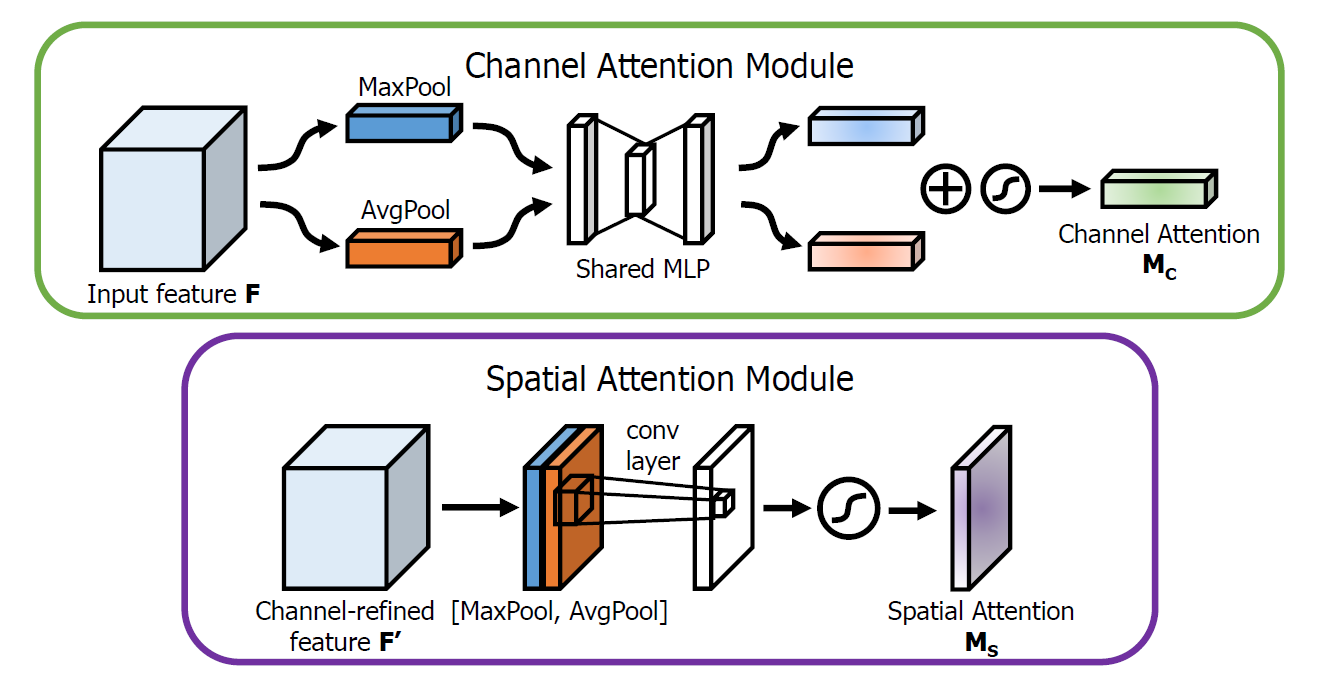
\includegraphics[width=0.88\textwidth]{figures/am.png}
	\caption{CAM和SAM结构示意图\cite{DBLP:conf/eccv/WooPLK18}}
	\label{fig:am机制}
\end{figure}

CAM通过全局池化操作和多层感知机对通道维度的信息进行了整合,
SAM通过全局池化操作和卷积操作对空间维度的信息进行了整合,具体工作原理如下:
\begin{align}
\mathbf{F}_{\mathbf{c}} &=\mathbf{M}_{\mathbf{c}}(F) \otimes F \\
\mathbf{F}_{\mathbf{s}} &=\mathbf{M}_{\mathbf{s}}\left(F\right) \otimes F \\
\mathbf{M}_{\mathbf{c}}(F) &=\mathbf{\sigma}(\mathbf{MLP}(\mathbf{GAP}(F))+\mathbf{MLP}(\mathbf{GMP}(F))) \label{eq8}\\
\mathbf{M}_{\mathbf{s}}(F) &=\mathbf{\sigma}\left(Conv\left(\mathbf{GAP}_\mathbf{c}\left(F\right) \oplus \mathbf{GMP}_\mathbf{c}\left(F\right)\right)\right) \label{eq9}
\end{align}

\noindent 其中$F \in R^{C \times H \times W}$表示输入特征图(C、H、W分别表示通道数和特征图的高度及宽度),
$\mathbf{M}_{\mathbf{c}} \in R^{C \times 1 \times 1}$和$\mathbf{M}_{\mathbf{s}} \in R^{1 \times H \times W}$
分别代表CAM和SAM。
$\otimes$表示元素乘法,经CAM和SAM处理后的输出特征图$\mathbf{M}_{\mathbf{c}}(F)$和$\mathbf{M}_{\mathbf{s}}\left(F\right)$
需要与输入特征图$F$相乘,保证输入和最终输出的大小和维度一致。
公式\ref{eq8}和\ref{eq9}展示了CAM和SAM的具体操作:
CAM先对输入特征图在空间域进行全局最大池化(global  max pooling,GMP)和全局平均池化(global average pooling,GAP),分别得到一个单通道向量,
再将该向量输入一个多层感知机进行通道方向的信息融合,最后将GMP和GAP的结果相加,
通过sigmoid激活函数得到$\mathbf{M}_{\mathbf{c}}(F)$;
SAM也对输入特征图进行了GMP和GAP,不同的是池化操作是在通道方向进行;
利用$\oplus$操作,将池化的结果进行叠加,然后利用卷积操作对空间维度的信息进行融合。

由于SAM模块中含有卷积操作,神经网络剪枝会对SAM模块产生影响,
所以在设置注意力模块时仅在“U”形\textsc{FlowDNN}的底部设置了SAM模块,其他skip connections仅嵌入CAM模块;
在进行神经网络剪枝时,与SAM模块相连的卷积层和逆卷积层不参与剪枝,保证SAM模块不受影响。
CAM模块通过多层感知机进行通道维度的信息融合,因此不受神经网络剪枝的影响。


\subsection{神经网络剪枝}
神经网络剪枝(network pruning)通过裁剪卷积层中卷积核大小或数量及其关联层参数大小,
减小模型的计算量和体积,从而加快模型部署后的推理速度,是一种减小模型大小和降低模型计算复杂度的常用方式。
在气动流场预测模型训练完成后,我们对网络进行了神经网络剪枝\cite{DBLP:conf/iclr/LiuSZHD19},
主要有两方面考虑:
a)一方面,相对于基线模型\textsc{FlowDNN}的网络参数较多。通过对网络进行剪枝,
可以证明\textsc{FlowDNN}对气动流场预测性能的提升不是简单的增加网络参数量;
b)另一方面,由于神经网络的冗余性,适当的剪枝并不会对预测精度产生明显的影响,
但是剪枝后模型的推理时间将有效减少。对于复杂的大规模气动流场模拟,剪枝对于提升预测性能意义重大。

神经网络剪枝要解决的核心问题就是“剪哪里”,
即评估卷积核重要性的标准,常见的标准有:内核权重的大小,特征映射激活值的均值、标准差和比例,激活值和预测值之间的互信息等。
本文采用了文献\cite{DBLP:conf/iclr/MolchanovTKAK17}的方法,
通过基于泰勒展开的方法近似评估每个卷积核被剪枝后损失函数的变化,进而根据卷积核的重要性对网络进行裁剪。
图\ref{fig:pruning}是神经网络剪枝的流程示意图:
1)载入训练好的模型;2)通过剪枝算法对每个卷积核的重要性进行评估;3)剔除重要性最低的卷积核;
4)利用训练数据对剪枝后的网络进行微调;
5)判断网络剪枝是否满足预设条件(参数量等),如果不满足,返回第二步;如果满足就结束网络剪枝。
 

\begin{figure}[htp]
	\centering
	%\includegraphics[width=0.42\textwidth]{data/MLP.pdf}
	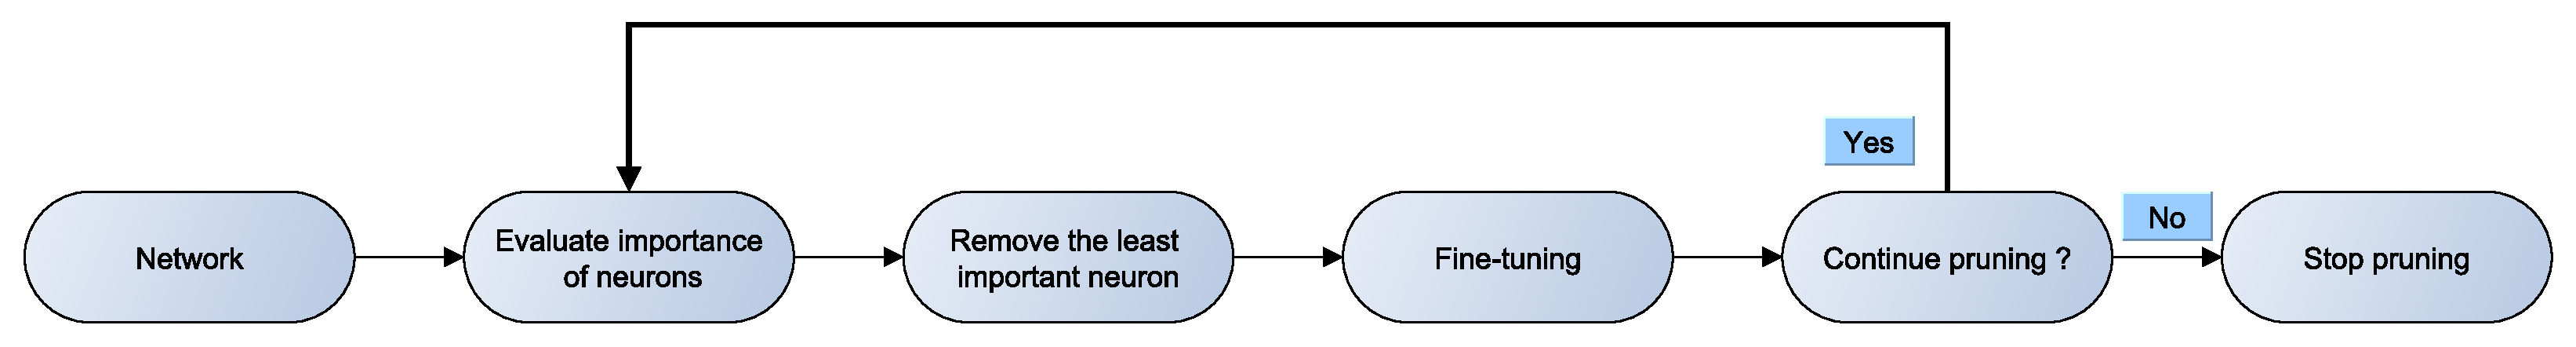
\includegraphics[width=0.99\textwidth]{figures/pruning_flow.pdf}
	\caption{神经网络剪枝流程示意图}
	\label{fig:pruning}
\end{figure}



\section{实验设置与结果分析}

\subsection{数据集与参数设置}

\subsubsection{基于LBM求解器生成数据集}
实验算例设置为二维定常不可压层流的外流问题,几何外形为不同形状的二维汽车外形。
我们使用基于LBM方法的开源库MECHSYS\footnote{ http://mechsys.nongnu.org}对二维流场进行模拟。
为了验证模型的泛化能力,我们将训练集设置为3000个简单几何体的组合形状,包括三角形、圆形、椭圆和方形等,不同样本中几何体大小和位置不同;验证集和测试集分别是22和44个不同形状的汽车外形。图\ref{fig:sample}是部分训练集样本和测试集数据样本可视化结果。

\begin{figure}[htb]
	\centering
	\subfloat[训练集]{\label{fig:training_sample}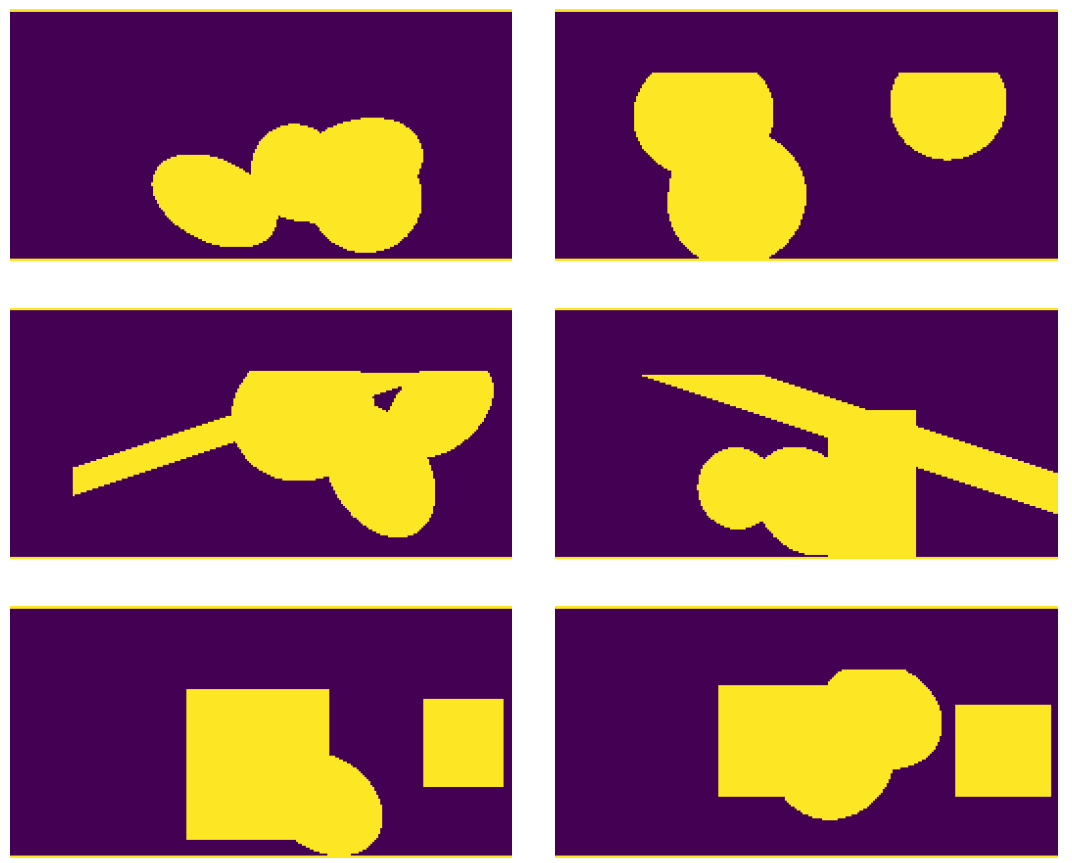
\includegraphics[width=0.42\textwidth]{figures/data/data_rep/training_sample/train_sample.png}} \qquad
	\subfloat[测试集]{\label{fig:testing_sample}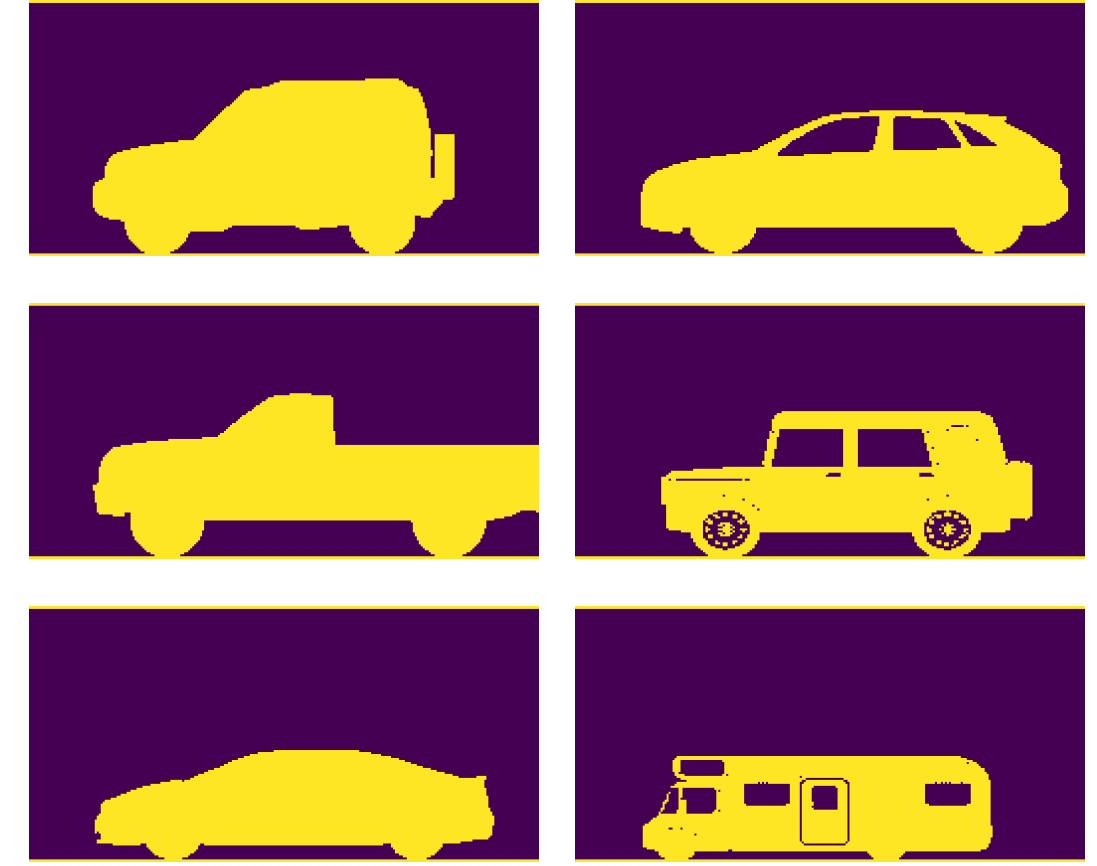
\includegraphics[width=0.42\textwidth]{figures/data/data_rep/training_sample/test_sample.png}} 
	\caption{训练集和测试集数据样本可视化示例}
	\label{fig:sample}
\end{figure}

在进行LBM流场模拟时,雷诺数设置为400以获取层流模拟结果;气流流向与x方向平行,采用D2Q9模型对速度矢量进行离散。
所有LBM求解程序都在GPU上并行执行,迭代10000时间步,保证计算结果的收敛性。
神经网络训练输入和输出特征图尺寸相同,输入为基于二元法表示的几何外形,输出为二维速度场,笛卡尔网格大小为256x128。


\subsubsection{参数设置}

\newcommand{\tabincell}[2]{\begin{tabular}{@{}#1@{}}#2\end{tabular}}
\begin{table}[htp]
	\setlength{\belowcaptionskip}{0.0cm}
	\caption{模型训练超参数设置 }
	\label{tab:parameters}
	\centering
	\begin{tabular}{p{1.9cm}p{1.6cm}p{1.2cm}p{1.4cm}p{1.6cm}p{1.2cm}p{1.4cm}}
		\toprule
		& \tabincell{c}{Learning \\ rate (Lr)}  & \tabincell{c}{Lr decay \\ interval} &  \tabincell{c}{Batch \\ size} & \tabincell{c}{Size of \\ the filters}  & \tabincell{c}{ Pruning \\ number}  & \tabincell{c}{Weights of \\ $L_{\rm{physical}}$} \\
		\midrule
		Optimum  &$4\times10^{-4}$  &	25 &	16 & 4 &1  & (1, 5, 25) $/$ 3  \\
		\midrule
		Tuning range & $10^{-5}$ \textasciitilde $10^{-3}$ 	&	20\textasciitilde 50 	&4\textasciitilde64  & 	2\textasciitilde8	 &1\textasciitilde5  &  - \\
		
		
		\bottomrule
	\end{tabular}
\end{table}

\textsc{FlowDNN}基于PyTorch深度学习框架编程实现,
在实验中,我们利用英伟达Tesla V100 GPU实现模型的训练、参数调优和神经网络剪枝。
深度学习训练有许多超参数,包括批大小学习率等,
表\ref{tab:parameters}展示了一些重要的超参数调优的范围以及最终的设置。
模型训练使用Adam优化算法,为了得到稳定收敛的结果,模型在数据集上训练400轮次(epoch)。
初始学习率设置为$4\times10^{-4}$,每25个epochs将学习率更新,乘以衰减因子0.9。
学习率衰减的好处是适应模型训练的特点,在前期加速模型训练,后期保证模型收敛至稳定状态。
批大小设置为16,意味着模型在进行推理时可以同时对16个不同初始条件流场进行预测。
在剪枝过程中,我们对每次剪枝的数量进行了探究,最终决定每次迭代只剪枝一个神经元,
因为一次剪枝过多会破坏神经网络结构,导致预测准确率急剧下降。每个剪枝迭代步之后,对剪枝后的网络进行微调,
训练40个epochs是神经网络收敛。
对激活函数,本文考虑两种常用的激活函数ReLU(rectified linear units)和ELU(exponential linear units),
其中ELU激活函数在文献\cite{DBLP:journals/corr/abs-1908-04387}中被推荐使用,两者的比较结果可见\ref{ac_effect}节。
对于损失函数的权重,我们先固定${\alpha _1}$为1,然后调整${\alpha _2}$和${\alpha _3}$使得损失函数的每一项在数值上对总的损失函数贡献相当;由于我们有损失函数有三项,将${\alpha _1}$、${\alpha _2}$和${\alpha _3}$分别除以3,即为最终损失函数的权重。




\subsubsection{性能评估标准}

\textbf{基线模型}

本文引入三个基线模型,用来比较和评估\textsc{FlowDNN}对稳态流场的预测结果:\\
(1) \texttt{C-Net}\cite{DBLP:conf/kdd/GuoLI16}:基于自编码器的流场预测方法,
	使用了3层卷积层和3层逆卷积层分别是实现对流场数据的编码与解码。\\
(2)	\texttt{T-Net}\cite{thuerey2019deep}:基于U-net改进的流场预测方法,
	基于深度神经网络推断RANS模型的流场压力场与速度场分布。\\
(3) \texttt{U-Net}\cite{DBLP:conf/miccai/RonnebergerFB15}:用于图像分割的经典深度神经网络,
	被广泛用于图像回归预测任务。

	




\textbf{流场预测结果评价指标}

对于深度神经网络模型的预测结果,本文使用平均相对误差(Mean Relative Error,MRE)比较预测流场和真值之间的差异,对气动流场的预测准确率进行总体的评估。
除了全场模拟结果,CFD领域专家通常对某些特定的区域感兴趣,比如流场边界层(即几何体表面附近流场),在RoI区域中流场变化剧烈,往往包含着更多有用的信息。对于本文使用的汽车外部流场,我们定义RoI区域如图\ref{fig:errors_area}中红色方框选中区域所示。RoI不是固定的,对于不用的汽车外形,红色方框自适应地恰好选中整个汽车。在确定了RoI之后,即可求得该区域的平均相对误差$\rm{MRE_{RoI}}$。
根据流体流动遵循的质量守恒定律和动量守恒定律,我们设计了${\rm{MRE}_{ma}}$和${\rm{MRE}_{mo}}$分别评测模型预测结果与真值的质量守恒一致性和动量守恒一致性。

\begin{figure}[htp]
	\centering
	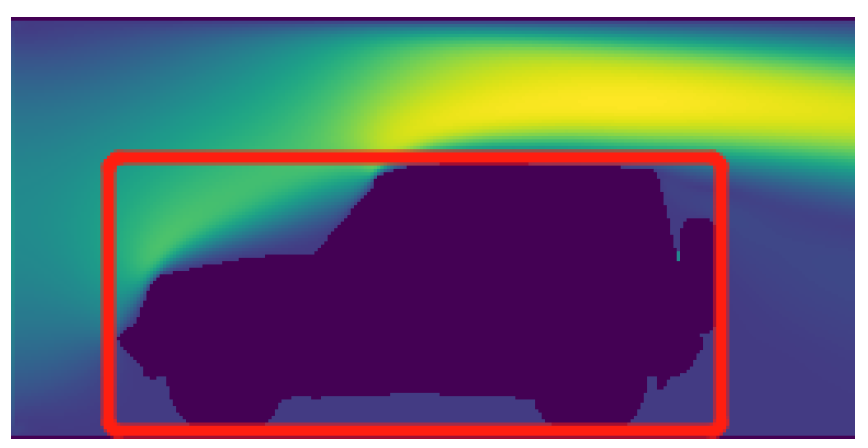
\includegraphics[width=0.44\textwidth]{figures/data/data_rep/errors.png}
	\caption{RoI示意图}	
	\label{fig:errors_area}
\end{figure}

在测试集有N个样本的情况下,对于二维流场有:
\begin{align}
MRE = { \frac{1}{N} \sum\limits_{l = 1}^N  \left( {\sum\limits_{i = 1}^{{n_x}} {\sum\limits_{j = 1}^{{n_y}} {\left( {\left| {u_{ij}^l - \overline u _{ij}^l} \right| + \left| {v_{ij}^l - \overline v _{ij}^l} \right|} \right)} } } / {{\sum\limits_{i = 1}^{{n_x}} {\sum\limits_{j = 1}^{{n_y}} {\left( {\left| {u _{ij}^l} \right| + \left| { v _{ij}^l} \right|} \right)} } }} \right) }
\end{align}

\begin{align}
MRE_{RoI} = { \frac{1}{N} \sum\limits_{l = 1}^N \left( { {\sum\limits_{i = 1}^{{n_s}} {\left( {\left|
					{u_{i}^l - \overline u _{i}^l} \right| + \left| {v_{i}^l - \overline v _{i}^l} \right|} \right)} } } /  {{ {\sum\limits_{i = 1}^{{n_s}}
				{\left( {\left| {u _{i}^l} \right| + \left| { v _{i}^l} \right|} \right)} } }} \right)}
\end{align}

\begin{align}
MRE_{ma} / MRE_{mo} = { \frac{1}{N} \sum\limits_{l = 1}^N  \left({\sum\limits_{i = 1}^{{n_x}} {\sum\limits_{j = 1}^{{n_y}} { {\left| {g_{ij}^l - \overline g _{ij}^l} \right| } } } } /  {{\sum\limits_{i =1}^{{n_x}} {\sum\limits_{j = 1}^{{n_y}} { {\left| {g _{ij}^l} \right|} } } }} \right)} 
\label{eq:mam}
\end{align}

\noindent 其中$n_s$表示在RoI中的格子数。在公式\ref{eq:mam}中,$g$和$\overline g$分别表示在真值和预测结果的每个格子点上质量(或动量)的变化值。



\subsection{实验结果与分析}

\subsubsection{总体预测性能比较}
通过大量实验,我们将基于不同深度学习方法的预测结果和基于LBM方法的求解器模拟结果进行了对比。
表\ref{tab:all_comp}展示了\textsc{FlowDNN}和基线模型在测试集上预测准确率,推理时间和模型参数量等方面的性能表现,其中AM表示嵌入了注意力模块,$P$代表神经网络剪枝;\textsc{FlowDNN}均使用物理损失函数进行训练。

\begin{table}[htp]
	\caption{不同深度学习方法的各项性能指标比较}
	
	\label{tab:all_comp}
	\centering
	
	\begin{tabular}{p{3.5cm}p{1.1cm}p{1.3cm}p{1.2cm}p{1.2cm}p{1.2cm}p{1.5cm}}
		\toprule
		\textbf{Method}  & \textbf{MRE} &  ${\textbf{MRE}_{RoI}}$ & $\textbf{MRE}_{ma}$ & $\textbf{MRE}_{mo}$ & \textbf{Runtime (ms)} & \textbf{Parameters (Mb)}\\
		\midrule
		LBM 				&	- &	-&	-&	-		&  3300$\times$16 	& -\\
		\textit{C-Net}   &	14.31\%&	30.99\% &	37.44\%&	45.60\%	&9.29    	& 180.25\\
		\textit{T-Net}   		&	24.65\%&	59.71\%&	79.09\%&	82.38\%	&  8.47 	& 7.45   \\
		\textit{U-Net}   &	14.74\%&	13.14\%&	30.78\%&	44.42\%	& 16.15      	&  32.96 \\
		\textsc{FlowDNN}   		&	7.91\%&	23.56\%& 18.28\%&	22.46\%	& \textbf{3.52}	& 13.70   \\
		\textsc{FlowDNN} w/ AM   		&5.34\% &9.16\% & 12.34\% & 15.69\%  & 4.51   	& 13.74   \\
		\textsc{FlowDNN} w/ AM \& $P$		&\textbf{4.77\%} &\textbf{8.87\%}&\textbf{12.14\%}&\textbf{14.63\%}  & \textbf{3.62}   	& \textbf{7.40}   \\
		%		Ours w/ AM \& $P^2$		&\textbf{5.20\%}  & \textbf{1.99}   	& 8.50   \\
		\bottomrule
	\end{tabular}
	
\end{table}

在模型参数量方面,因为\texttt{C-Net}网络架构中使用了全连接层,每个神经元与其前一层的所有神经元进行全连接,导致网络参数量远大于其他模型,大小为180.25Mb。
在基线模型中,\texttt{T-Net}模型参数量最小为7.45Mb,约是剪枝之前\textsc{FlowDNN}模型大小的一半。
此外,在\textsc{FlowDNN}嵌入注意力模块之后,模型大小几乎没有改变,体现出轻量级注意力模块的灵活性。
在推理时间方面,在利用深度学习模型进行流场预测时我们将批大小设置为16,即一次推理过程可以得到16个算例的预测结果。
对于每个算例,LBM求解器通过迭代计算求解控制方程得到收敛的二维速度场结果,在GPU测试平台上程序的平均运行时间约为3300ms。
对于深度学习预测模型,尽管\texttt{U-Net}模型参数不是最大,但推理时间最长,这可能和网络中卷积核的大小和采样的方式方式有关。
\textsc{FlowDNN}的推理时间最短为3.52ms,在嵌入注意力模块之后推理时间增加了近四分之一,经过神经网络剪枝后推理时间基本和嵌入注意力模块之前相当。

对于指标$MRE$和$MRE_{RoI}$,模型的预测结果基本上是$MRE_{RoI}$远大于$MRE$,
说明对于气动流场而言,几何体表面附近相较于远场更难以预测,反映出该区域速度变化更加剧烈,这符合流体流动的一般特点。
然而我们观察到\texttt{U-Net}对于全场和RoI区域的预测性能接近甚至在RoI区域更准确,这一结果可能和\texttt{U-Net}的网络结构相关,但具体的原因需要进一步探究。
相较于三种基线模型,在不引入注意力机制和神经网络剪枝的情况下,使用物理损失函数训练\textsc{FlowDNN}可以使$MRE$降低至7.91\%,接近三种基线模型中表现最好的\texttt{C-Net}的一半。
但是\textsc{FlowDNN}对RoI区域的预测效果并不理想,$MRE_{RoI}$仅为23.56\%,不仅远大于\texttt{U-Net}的13.14\%,而且是$MRE$预测误差的三倍。因此,本文引入了注意力机制希望能提升\textsc{FlowDNN}对几何体表面附近流场的预测效果。



对于指标$MRE_{ma}$和$MRE_{mo}$,不同深度学习方法的预测结果均体现出$MRE_{mo}$大于$MRE_{ma}$的趋势,可以得知相较于质量守恒,预测结果往往更难以保证动量守恒的一致性。由于\textsc{FlowDNN}均是使用物理损失函数训练,所以与基线模型相比,$MRE_{ma}$和$MRE_{mo}$误差比较小。关于损失函数对预测结果的影响可见\ref{phy_effect}节。此外,注意力模块也有效降低了$MRE_{ma}$和$MRE_{mo}$误差。



\begin{figure}[htp]
	\centering
	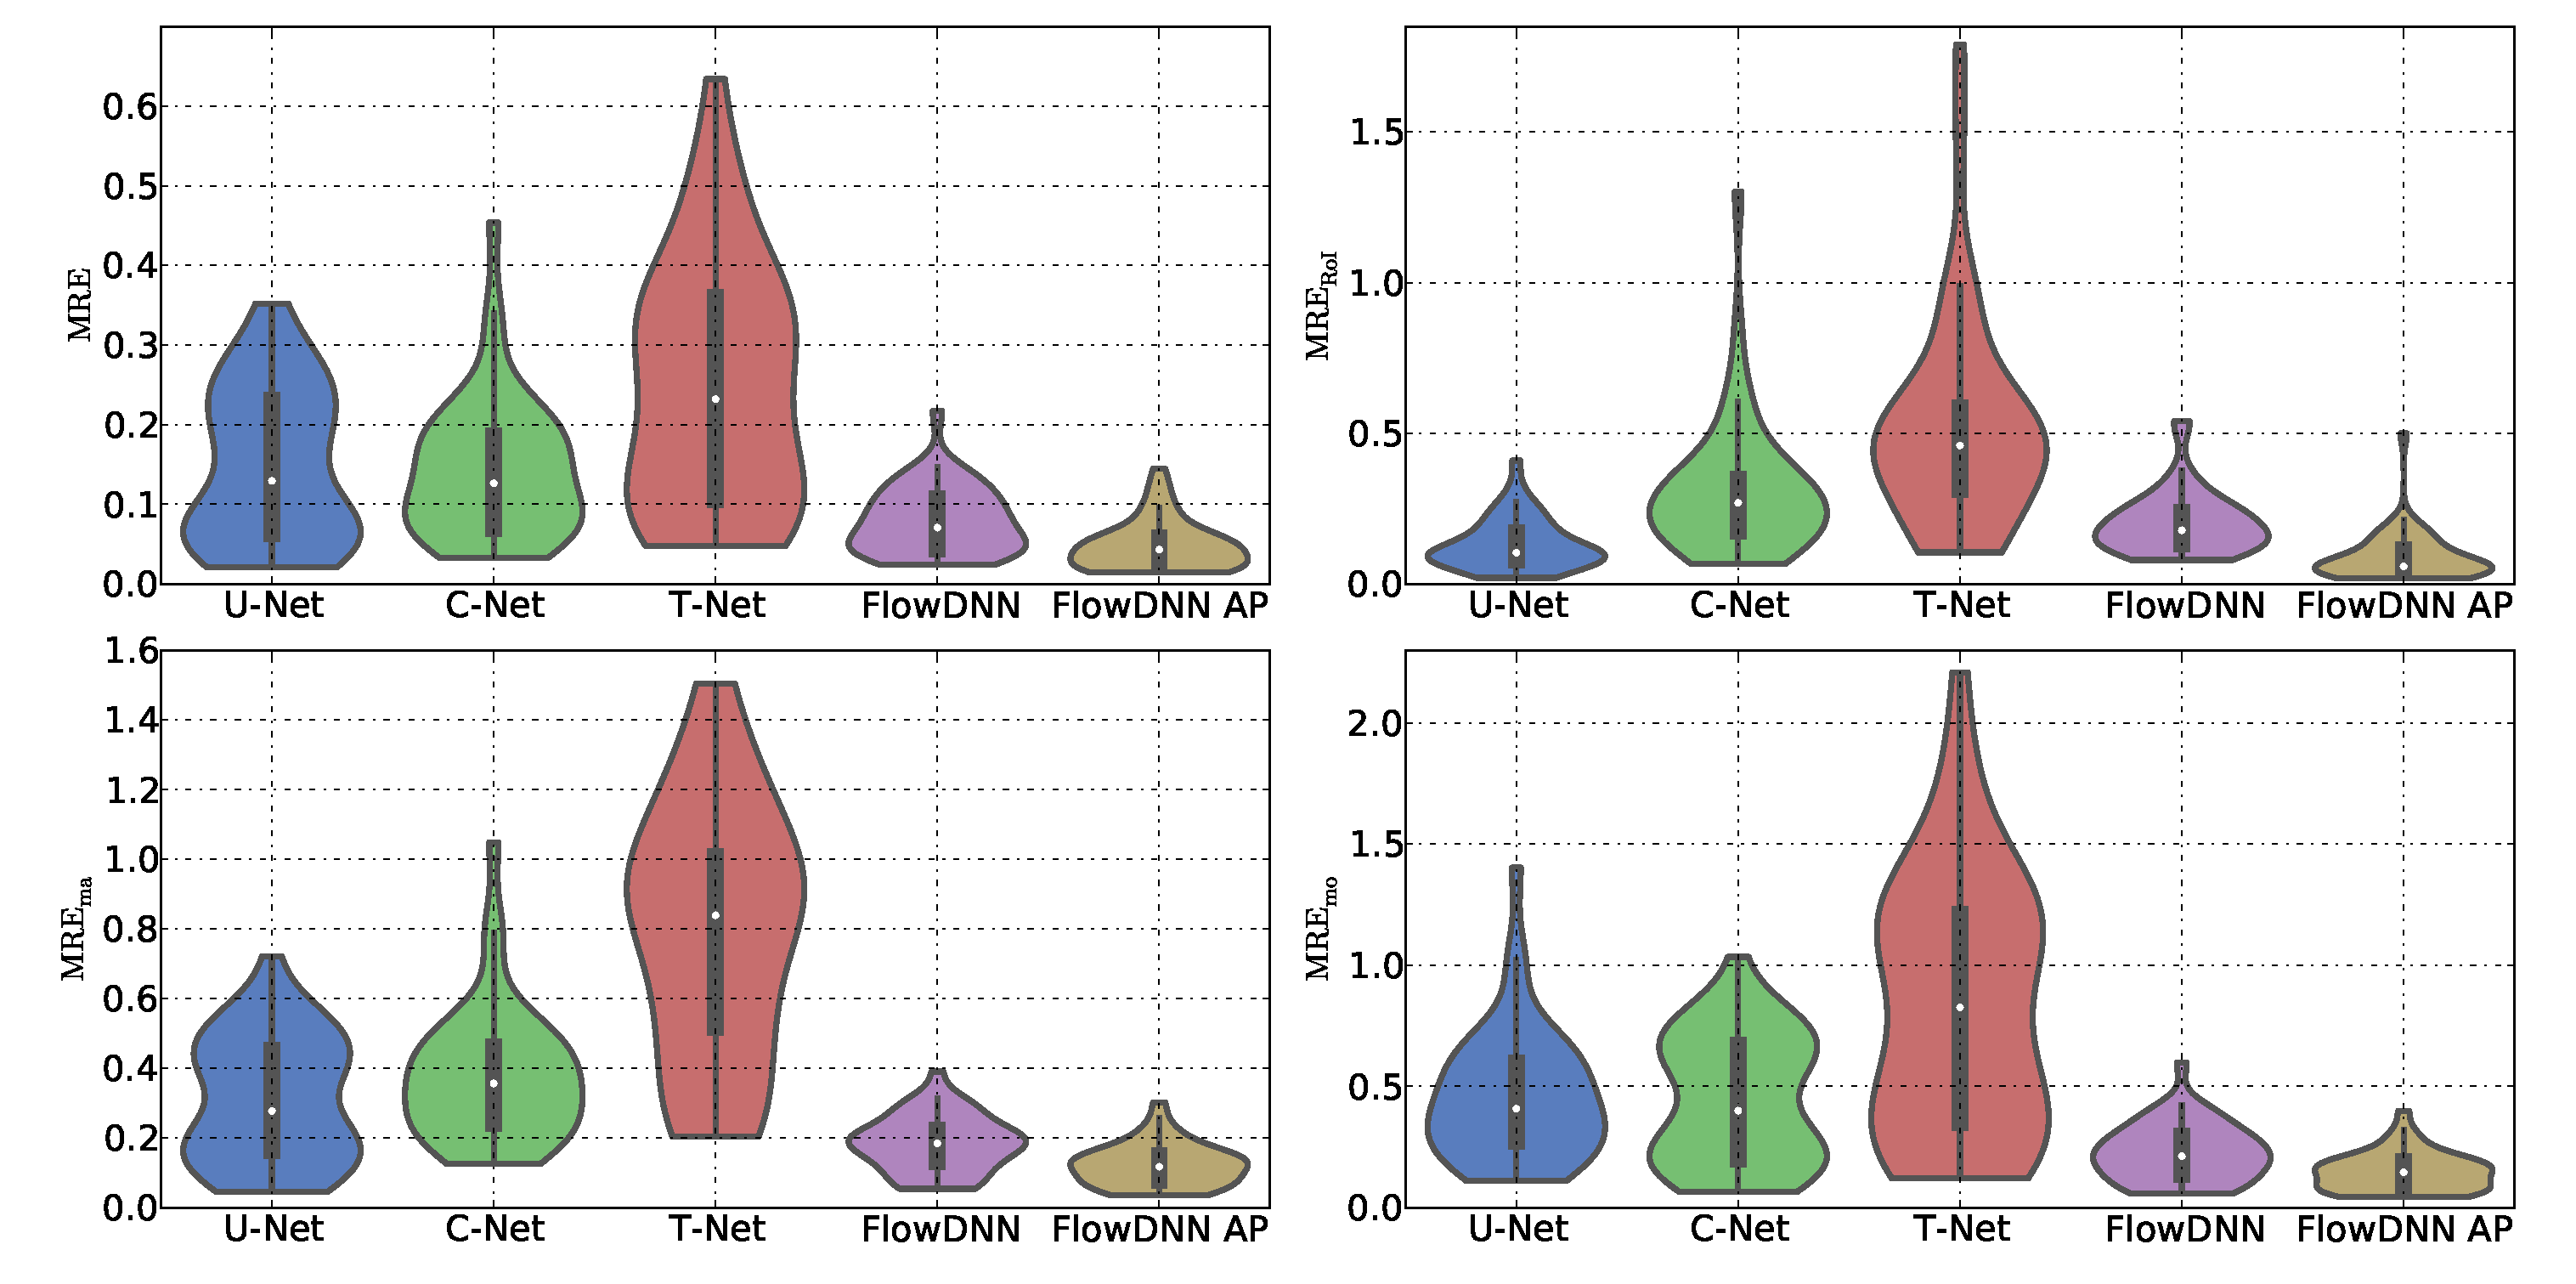
\includegraphics[width=0.98\textwidth]{./figures/data/all_violin.pdf}
	\caption{不同深度学习方法的预测性能指标在测试集上的分布}
	\label{fig:overall_violin}
\end{figure}


图\ref{fig:overall_violin}展示了$MRE$、$MRE_{RoI}$、$MRE_{ma}$和$MRE_{mo}$四种指标在测试集上分布情况。
小提琴图外围的曲线宽度代表数据点分布的密度,内部的黑色长条表示中间二分之一的样本分布的范围,白点表示所有样本的中位数。
观察三种基线模型的预测结果分布,除了\textit{U-Net}在指标$MRE_{RoI}$上表现比较稳定之外,
其他情况的预测误差都表现出很大的波动,即在某些样本上模型预测性能较好,在另一些样本上预测性能则较差,
比如\textit{U-Net}对某个算例的预测结果的$MRE$误差甚至超过了50\%。
相比之下,\textsc{FlowDNN}不仅在各项性能指标上平均误差较小,而且表现出良好的预测稳定性,对于测试集上不同的算例,
\textsc{FlowDNN}能将流场预测结果的误差控制在较小的范围。

\begin{table}[htp]
	\caption{不同深度学习方法的二维速度场预测结果}
	
	
	\label{tab:total_comp_case}
	\centering
	\begin{tabularx}{14cm}{p{0.8cm}p{1.9cm}p{1.5cm}p{1.5cm}p{1.5cm}p{1.5cm}p{2.6cm}}
		\toprule
		& ~~~~~~~LBM  & ~~~~\textit{U-Net} & ~~~~\textit{C-Net} & ~~~~\textit{T-Net} & ~~\textsc{FlowDNN} & ~~\textsc{FlowDNN} AP   \\
		\midrule
		
		racing &\multicolumn{6}{l}{
			\begin{minipage}{\textwidth}
				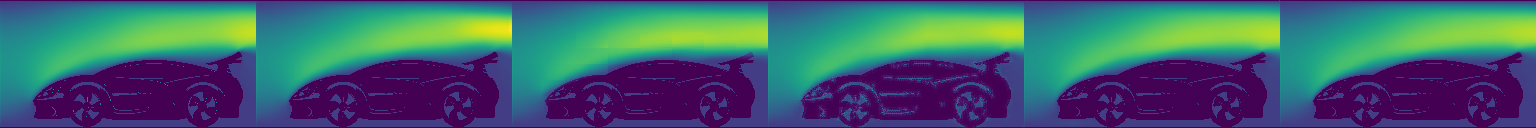
\includegraphics[width=0.82\textwidth]{./figures/data/pic_xin/final_35.png}
			\end{minipage}}
			\\
			
			saloon &\multicolumn{6}{l}{
				\begin{minipage}{\textwidth}
					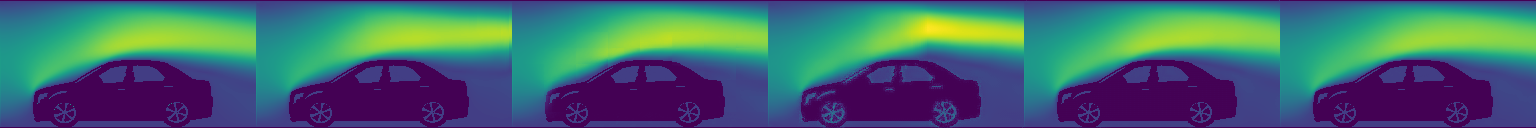
\includegraphics[width=0.82\textwidth]{./figures/data/pic_xin/final_32.png}
				\end{minipage}}
				\\
				jeep &\multicolumn{6}{l}{
					\begin{minipage}{\textwidth}
						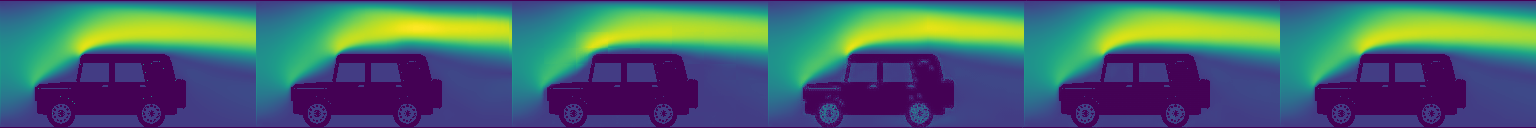
\includegraphics[width=0.82\textwidth]{./figures/data/pic_xin/final_20.png}
					\end{minipage}}
					\\
					pickup &\multicolumn{6}{l}{
						\begin{minipage}{\textwidth}
							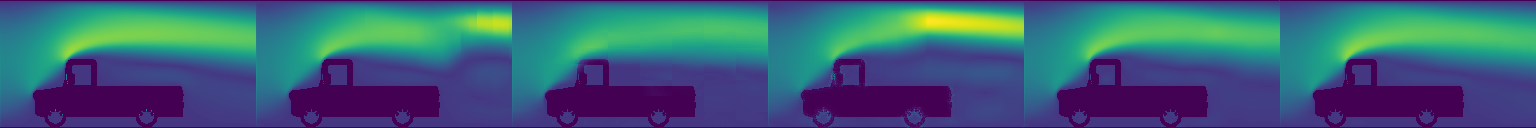
\includegraphics[width=0.82\textwidth]{./figures/data/pic_xin/final_39.png}
						\end{minipage}}
						\\	
						bus &\multicolumn{6}{l}{
							\begin{minipage}{\textwidth}
								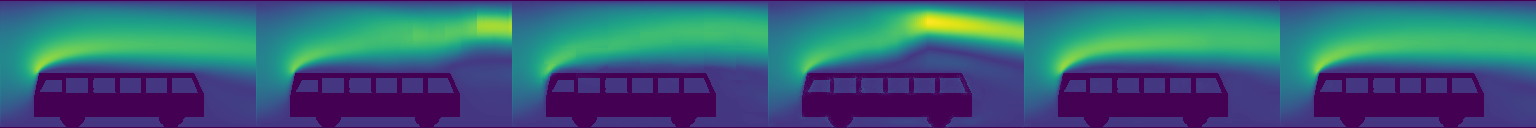
\includegraphics[width=0.82\textwidth]{./figures/data/pic_xin/final_8.png}
							\end{minipage}}
							\\
							\bottomrule
						\end{tabularx}
					\end{table}

表\ref{tab:total_comp_case}展示了基于不同深度学习方法预测的流场速度场的可视化结果。\textsc{FlowDNN} AP表示使用了注意力机制和神经网络剪枝的\textsc{FlowDNN}。
对于不同的汽车外形,\textsc{FlowDNN}的二维速度场预测结果都体现出与LBM求解器模拟结果的高度一致性。
观察\texttt{U-Net}和\texttt{T-Net}的预测结果,我们发现对于部分汽车外形如pickup(皮卡)和bus(公共汽车),
几何体上方的流场会出现明显的断层,原因可能是模型的泛化能力有限,对于不同的汽车外形的预测结果可能出现过拟合现象。
虽然\texttt{C-Net}对流场速度场的预测结果没有出现断层的现象,
但是可以看出速度场可视化结果模糊,这是预测结果精度不够导致的。
此外,\texttt{C-Net}预测结果具有明显的分块现象,这和\texttt{C-Net}在进行卷积操作时使用了较大的步长有关,
导致数据的局部性信息有较大程度的损失。



为了对不同深度学习方法的流场预测结果进行进一步分析,本文比较了不同深度学习方法的二维速度场预测结果与真值的差异。
如表\ref{tab:total_comp_case_error}所示,深度学习模型的预测误差主要集中在几何体周围以及几何体尾部区域。
这是由于流体绕物流动时会产生涡旋区,主要集中在几何体表面边界层。
这随着流动的进行,涡旋会与物体脱离,继而在物体后部形成不稳定带旋涡的尾流。
所以在几何体周围以及几何体尾部区域中,流体的运动规律更加复杂,导致模型预测误差较大。
对比\textsc{FlowDNN}和三个基线模型的预测结果与真值的差异,
可以直观地看出\textsc{FlowDNN}能够对二维速度场进行准确的预测,有效降低几何体周围以及几何体尾部区域的预测误差。




\begin{table}[htp]
	\caption{不同深度学习方法的二维速度场预测结果与真值的差异比较}
	\label{tab:total_comp_case_error}
	\centering
	\begin{tabularx}{14cm}{p{0.8cm}p{2cm}p{2cm}p{2cm}p{2cm}p{2.4cm}}
		\toprule
		&  ~~~~~~~\textit{U-Net} & ~~~~~~~\textit{C-Net} & ~~~~~~~\textit{T-Net} & ~~~\textit{FlowDNN} & ~~~\textit{FlowDNN AP}   \\
		\midrule
		
		racing &\multicolumn{5}{l}{
			\begin{minipage}{\textwidth}
				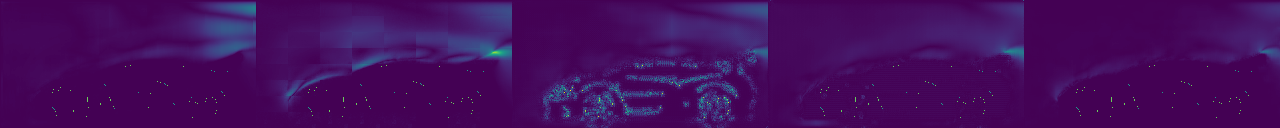
\includegraphics[width=0.82\textwidth]{./figures/data/pic_xin_error/final_35.png}
			\end{minipage}}
		\\
		
		saloon &\multicolumn{5}{l}{
			\begin{minipage}{\textwidth}
				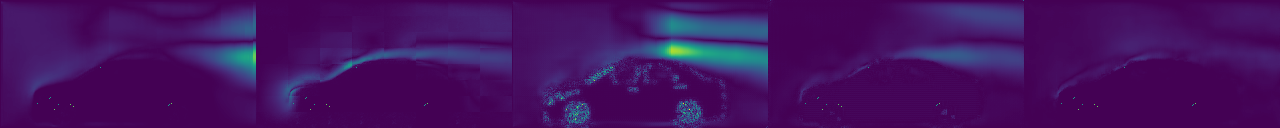
\includegraphics[width=0.82\textwidth]{./figures/data/pic_xin_error/final_32.png}
			\end{minipage}}
		\\
		jeep &\multicolumn{5}{l}{
			\begin{minipage}{\textwidth}
				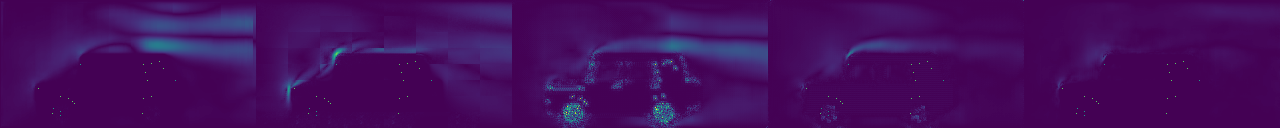
\includegraphics[width=0.82\textwidth]{./figures/data/pic_xin_error/final_20.png}
			\end{minipage}}
		\\
		pickup &\multicolumn{5}{l}{
			\begin{minipage}{\textwidth}
				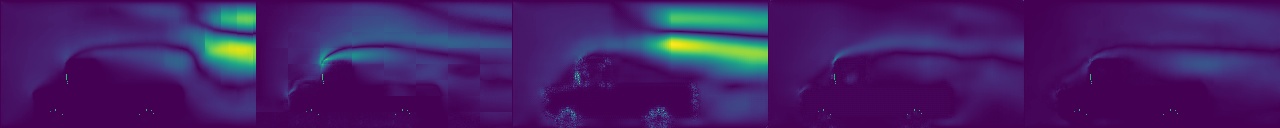
\includegraphics[width=0.82\textwidth]{./figures/data/pic_xin_error/final_39.png}
			\end{minipage}}
		\\	
		bus &\multicolumn{5}{l}{
			\begin{minipage}{\textwidth}
				\includegraphics[width=0.82\textwidth]{./figures/data/pic_xin_error/final_8.png}
			\end{minipage}}
		\\
		\bottomrule
	\end{tabularx}
\end{table}


\subsubsection{物理损失函数}\label{phy_effect}

为了探究物理损失函数对流场预测结果的影响,尤其是对预测结果和CFD求解器模拟结果的物理一致性的影响,
本文分别使用$L_{physical}$和$L_{1}$损失函数对\textsc{FlowDNN}进行了训练。

\begin{figure}[htp]
	\centering
	\includegraphics[width=0.58\textwidth]{./figures/data/data_pre/loss_comp.pdf}
	\caption{不同损失函数对流场预测结果的影响}
	\label{fig:phy_bar_comp}
\end{figure}

\noindent 图\ref{fig:phy_bar_comp}展示了不同损失函数在$MRE$、$MRE_{RoI}$、$MRE_{ma}$和$MRE_{mo}$四项性能指标的表现。
可以看到,相对于传统的$L_{1}$损失函数,使用物理损失函数训练预测模型可以有效地降低$MRE_{ma}$(从37.83\%降低至18.28\%),
质量守恒误差减小了一半。
物理损失函数对降低动量守恒误差$MRE_{mo}$也有一定效果,
我们分析$L_{physical}$对$MRE_{ma}$和$MRE_{mo}$影响不同的原因和损失函数权重有关。

我们对物理损失函数对预测结果的物理一致性的影响进行了进一步探究。
图\ref{fig:phy_hotmap}展示了真值和不同损失函数预测结果在每个格子点上质量和动量的变化值。
可以看出质量和动量的变化主要集中在定义的RoI区域和流场尾部区域,
这也导致了使用物理损失函数训练的流场预测模型,其预测结果的$MRE$并没有显著降低,
而$MRE_{RoI}$从42.23\%降低至23.56\%。
此外,我们观察到$L_{1}$的预测结果会出现不符合流体流动规律的情况,即$\Delta \mathrm{mass}$位于几何体内部,
物理损失函数可以有效减少这种情况的发生,增强预测结果和CFD求解器模拟结果的物理一致性。


\begin{figure}[htp]
	\centering
	\includegraphics[width=0.62\textwidth]{./figures/data/loss_comp_case/loss_comp.png}
	\caption{不同损失函数对流场预测结果物理一致性的影响}	
	\label{fig:phy_hotmap}	
\end{figure}

\subsubsection{注意力机制}
为了提升模型的表示能力和非线性,提高\textsc{FlowDNN}对RoI区域的预测精度,
我们在\textsc{FlowDNN}的skip connections上嵌入了SAM和CAM模块。
从表\ref{tab:all_comp}中可知,嵌入注意力模块的\textsc{FlowDNN}有效增加了神经网络对RoI区域信息的提取能力,使RoI区域的平均相对误差$MRE_{RoI}$下降至9.16\%,同时提升了全场的预测准确率。
图\ref{fig:attention_violin}展示了在使用和不使用注意力模块的情况下,\textsc{FlowDNN}的$MRE_{RoI}$误差在测试集上的分布。
在未使用注意力机制之前,测试集上$MRE_{RoI}$误差集中在18\%左右;使用注意力机制之后,$MRE_{RoI}$误差集中在6\%左右,而且误差分布更加集中,提升了\textsc{FlowDNN}的流场预测稳定性。

\begin{figure}[htp]
	\centering
	\includegraphics[width=0.58\textwidth]{./figures/data/data_pre/error_s_compare_violin.pdf}
	
	\caption{注意力机制对$\rm{MRE_{RoI}}$在测试集上分布的影响}
	\label{fig:attention_violin}
\end{figure}

图\ref{fig:attention_val_loss_comp}展示了注意力机制对预测模型训练的影响。
相比不使用注意力机制的情况,嵌入了CAM和SAM模块的\textsc{FlowDNN}随着训练的进行收敛地更快,
在50个epoch时验证上的损失函数已经收敛到较低的水平,在150个epoch时验证集上的误差已经趋于稳定。
对比两条曲线的振幅,嵌入注意力模块的蓝线在垂直方向上的振幅更小,模型训练过程更加稳定。
在两条误差曲线都趋于稳定时,使用注意力模块的\textsc{FlowDNN}的误差收敛至更低的水平。

\begin{figure}[htp]
	\centering
	\includegraphics[width=0.58\textwidth]{./figures/data/am_comp.pdf}
	\caption{注意力机制对模型训练的影响}
	\label{fig:attention_val_loss_comp}
\end{figure}

由此可见,在\textsc{FlowDNN}中合理地嵌入注意力模块,不仅能大幅提升模型在RoI区域的预测精度,
还有助于加速模型训练收敛,缩短模型训练的时间,同时提高模型的预测稳定性。


\subsubsection{激活函数}\label{ac_effect}
激活层是深度神经网络的重要组成部分,对保证神经网络的非线性预测能力和提升神经网络模型的预测效果有重要影响。
本文比较了常用于气动预测模型的ReLU和ELU两种激活函数对气动流场预测模型的影响。
图\ref{fig:activation_intro}展示了两种激活函数的工作原理。

对ReLU激活函数有:
\begin{equation}
\varphi(x)=\max (0, x)
\end{equation}

\noindent 对ELU激活函数有:
\begin{equation}
\varphi(x)=\left\{\begin{array}{ll}
x & \text { if } x>0 \\
\alpha\left(e^{x}-1\right) & \text { if } x \leq 0
\end{array}\right.
\end{equation}

\noindent ReLU和ELU的x > 0 的部分作用效果是相同的,保留神经元的原始输入(y = x),都能有效克服梯度消失的问题\cite{2010Rectified};
在x < 0的部分,ReLU会将神经元的输出置为0,ELU则将输出映射到(-1,0)之间。


\begin{figure}[htb]
	\centering
	\subfloat[]{\label{fig:relu}\includegraphics[width=0.38\textwidth]{figures/ReLU.png}} \qquad
	\subfloat[]{\label{fig:elu}\includegraphics[width=0.38\textwidth]{figures/ELU.png}} 
	\caption{ReLU和ELU激活函数}
	\label{fig:activation_intro}
\end{figure}


图\ref{fig:activation}展示了ReLU和ELU两种激活函数对模型训练的影响。
为了保证模型收敛和避免模型训练产生梯度爆炸,
在激活函数进行处理之前我们对输入数据进行了批标准化(batch normalization,BN)。
在使用BN的情况下,使用ReLU作为激活函数模型随着训练收敛地更快;
训练稳定后,在测试集上的误差也小于使用ELU作为激活函数的情况。
我们分析ELU激活函数表现较差的原因可能是ELU本身能够将激活单元的输出均值往0推近,
和批标准化作用相似。所以ELU配合BN操作使用时,因为多次数据标准化处理,预测性能反而会较差。
因此我们对仅使用ELU激活函数的情况进行了测试,结果表明,仅使用ELU和ReLU+BN的效果相当。
考虑到ReLU激活函数能够将部分神经元输出置为0,增加神经网络的稀疏性,有利于神经网络剪枝,因此本章选取其作为激活函数。

\begin{figure}[htp]
	\centering
	\includegraphics[width=0.58\textwidth]{./figures/data/activation_comp.pdf}
	\caption{不同激活函数对模型训练的影响}
	\label{fig:activation}	
\end{figure}


\subsubsection{神经网络剪枝}

在选定损失函数,利用注意力机制对\textsc{FlowDNN}进行优化之后,我们对\textsc{FlowDNN}进行了神经网络剪枝。
引入神经网络剪枝主要出于两方面的考虑:
一方面剪枝后的预测模型参数减少,可以证明\textsc{FlowDNN}的预测性能提升不是简单地增加参数量;
另一方面,通过神经网络剪枝精简网络结构,加快预测模型推理速度。

\begin{figure}[htp]
	\centering
	\includegraphics[width=0.58\textwidth]{./figures/data/pruning_result.pdf}
	\caption{网络剪枝对$MRE$的影响}
	\label{fig:pruning_result}	
\end{figure}

图\ref{fig:pruning_result}展示了神经网络剪枝对\textsc{FlowDNN}预测结果的平均相对误差的影响。
其中平行于坐标横轴的是剪枝前\textsc{FlowDNN}的MRE误差,随着剪枝的进行,模型的MRE误差一直在基线上下波动;
在剪枝神经元数量超过500之后,随着剪枝继续进行,破坏了神经网络结构,导致MRE误差急剧上升。
本文选取MRE误差最小的剪枝模型作为最终的气动流场预测模型,整个二维速度场预测结果的平均相对误差仅为4.77\%。


\section{本章小结}

本章针对传统CFD方法进行流场模拟效率低的问题,
提出一种基于深度卷积网络的端到端流场预测方法。
首先分析了基于深度卷积网络进行流场预测的优势,对比了流场模拟任务和传统图像转换任务的相似点与不同点。
其次研究了基于笛卡尔网络的流场数据表示方法,包括SDF方法和二元法。
然后提出了基于U-net网络的气动流场预测模型\textsc{FlowDNN},具体包括:
针对流体运动特点,通过改进U-net网络架构;
基于流体流动的物理规律,提出融合物理损失项和传统$L_1$损失项的物理损失函数;
针对边界层等RoI区域预测准确率低的问题,引入注意力模块;
通过神经网络剪枝进一步优化模型预测效率。
最后定义了新的流场预测结果评价指标,与传统CFD求解器和三个基线模型进行了全面的性能比较。

实验表明,相对于三个基线模型,\textsc{FlowDNN}在测试集上的全场预测准确率、RoI区域准确率更高,
预测结果与CFD模拟结果的物理一致性更高;
与基于LBM的传统CFD方法相比,流场模拟效率提升14000x,同时将预测误差控制在5\%以内。



\chapter{基于图神经网络的流场模拟加速方法}

本章介绍了基于图神经网络的气动流场模拟加速方法,
首先利用CFD网格生成软件在算例几何模型上生成非结构网格,
基于网格单元拓扑连接信息、边界条件和初始条件提取图神经网络训练的输入数据;
利用CFD求解器获取图神经网络训练的真值。
然后基于图卷积神经网络设计了气动流场模拟加速模型,在模型训练完成后,
使用CFD求解器对气动流场模拟加速模型的输出结果进行优化。
最后在测试集上比较了气动流场模拟加速方法与传统CFD数值模拟方法的气动流场模拟效率。

\section{引言}

\subsection{动机分析}

利用深度学习方法对气动流场进行预测的主要思想是将气动流场模拟问题转化为图像回归预测问题,
因此需要将流场数据转化为矩阵的形式。
在处理流场中非结构数据时,则需要通过采样的方式将数据转化为结构规则的笛卡尔网格形式,
这样就会导致预测的结果在平滑区域(远场)过采样,而在流场边界层(几何体附近区域)欠采样,
导致预测流场结果在几何体周围轮廓模糊,不能真实的反映物理量在边界层的分布。
在传统基于网格的CFD模拟方法中,
一般通过加密边界层的网格密度以更加细致地捕捉边界层的速度和压力等物理量的变化,
使用均一的粗粒度的网格进行模拟根本不能得到准确的结果甚至导致计算不收敛。
此外,流场预测结果由深度学习模型输出,在复杂流动条件下,无法保证深度学习模型能够对流体运动规律进行准确学习,输出符合流体运动规律的预测结果。

基于以上考虑,本文在利用图神经网络进行流场模拟方面进行了探索,对气动流场模拟的效率和预测结果的有效性进行了权衡,
提出了基于图神经网络的流场模拟加速方法。

\subsection{研究思路}
与基于传统卷积神经网络的流场预测方法相比,基于图神经网络的流场模拟加速方法主要有两点不同:
1)流场数据表示方法通用性更强。
无论是结构网格还是非结构网格,利用图能够灵活地对网格单元的拓扑结构进行表示,
边界条件和初始条件可以处理为节点特征向量。
由于图结构利用网格对流场域进行了全尺寸模拟,不需要利用采样方法将流场表示为笛卡尔网格,
所以最大程度保留了原始流场数据中的信息,一些控制流体流动的全局变量也可以在图神经网络训练时用于每一个图节点上。
2)从根本上保证流场模拟结果的有效性。
利用CFD求解器对深度学习模型的预测结果进行优化,将计算收敛的结果作为最终的流场预测结果。
虽然深度学习模型在此方法中只是作为加速模块部分代替了CFD求解器的工作,
导致气动流场模拟效率低于基于深度学习的流场预测方法,
但由于气动流场模拟结果最终由CFD求解器输出,因此输出结果满足求解器计算收敛条件和流体流动物理规律。

由于图神经网络进行训练时需要保证图的拓扑结构保持不变,
因此本章主要针对给定几何外形在不同流动条件下气动流场模拟效率进行了研究。



\subsection{OpenFOAM网格数据结构}\label{meshstructure}
本文基于OpenFOAM软件进行网格生成和流场模拟。
OpenFOAM是基于C++程序语言开发用于场运算和操作的类库,主要包括两大类:求解器(solvers)和工具(utilities)。
用户可以根据特定的连续介质流体力学问题在标准的求解器基础上进行开发。工具主要有前处理工具和后处理工具两类。
前处理工具包括几何处理、网格处理、边界条件设置等,后处理工具包括数据提取与绘图、可视化处理等。
OpenFOAM主要网格文件及其包含的信息如表\ref{tab:openfoammesh}所示。

\begin{table}[htp]
	\setlength{\belowcaptionskip}{0.0cm}
	\caption{OpenFOAM网格文件信息}
	\label{tab:openfoammesh}
	\centering
	\begin{tabular}{c|c}
		\toprule
		文件 & 存储信息\\
		\midrule
		points  & 所有节点的三维坐标\\
		\midrule
		faces & 构造面单元的节点编号\\
		\midrule
		owner & 与面单元相对应owner体单元编号\\
		\midrule
		neighbour & 与面单元相对应neighbour体单元编号\\
		\midrule
		boundary & 边界条件设置\\		
		\bottomrule
	\end{tabular}
\end{table}

\texttt{points}文件以矢量场的形式存储所有节点坐标,单位为米,
文件主要内容如图\ref{fig:points_file}所示,节点的编号即为其坐标数据在points列表中的位置,初始编号为0。

\begin{figure}[htp]
	\centering
	\includegraphics[width=0.72\textwidth]{./figures/points.png}
	\caption{points文件结构}
	\label{fig:points_file}	
\end{figure}

\texttt{faces}文件存储面单元-节点拓扑结构数据,文件主要内容如图\ref{fig:faces_file}所示。面单元最少由3个节点组成(三角形),其构造节点总数为每一行数据第一个整数(任意不小于3的值),每一行括号内的整数为面单元构造节点的编号,表示其在points列表中的位置。
面单元的编号即为数据在faces列表中的位置,初始编号为0。整个faces列表包含边界面单元。

\begin{figure}[htp]
	\centering
	\includegraphics[width=0.72\textwidth]{./figures/faces.png}
	\caption{faces文件结构}
	\label{fig:faces_file}	
\end{figure}

如图\ref{fig:owner_neighbor}所示,owner体单元与neighbour体单元的标识基于公共面单元face外法向量($S_f$)的方向,即由owner单元指向neighbour单元。owner单元与neighbour单元有时亦被称为左单元与右单元。


\begin{figure}[htb]
	\centering
	\subfloat[]{\label{fig:on_2d}\includegraphics[width=0.45\textwidth]{figures/owner_neighbour_2d.png}} \qquad
	\subfloat[]{\label{fig:on_3d}\includegraphics[width=0.45\textwidth]{figures/owner_neighbour.png}} 
	\caption{面的owner与neighbor的关系}
	\label{fig:owner_neighbor}
\end{figure}

\texttt{owner}文件存储owner单元-面单元拓扑结构数据,文件主要内容如图\ref{fig:owner_file}所示。owner列表存储相对应面单元的owner单元编号,初始编号为0,owner列表的位置对应面单元的编号,亦对应于其在faces列表中的位置。任何一个面单元总存在一个owner单元,因此owner单元总数与面单元总数nFaces相等。

\begin{figure}[htp]
	\centering
	\includegraphics[width=0.72\textwidth]{./figures/owner.png}
	\caption{owner文件结构}
	\label{fig:owner_file}	
\end{figure}

\texttt{neighbour}文件存储neighbour单元-面单元拓扑结构数据,文件主要内容如图\ref{fig:neighbour_file}所示。neighbour列表存储相对应面单元的neighbour单元编号,初始编号不为0,neighbour列表的位置对应面单元的编号,亦对应于其在faces列表中的位置。需要特别说明的是,因为边界面单元没有neighbour单元,neighbour单元总数与内部面单元总数nInternalFaces相等。

\begin{figure}[htp]
	\centering
	\includegraphics[width=0.72\textwidth]{./figures/neighbour.png}
	\caption{neighbour文件结构}
	\label{fig:neighbour_file}	
\end{figure}

\texttt{boundary}文件存储整个网格的边界信息,比如边界区域名称、边界类型type、面单元个数nFaces以及起始面单元编号startFace等,文件主要内容如图\ref{fig:boundary_file}所示。

\begin{figure}[htp]
	\centering
	\includegraphics[width=0.72\textwidth]{./figures/boundary.png}
	\caption{boundary文件结构}
	\label{fig:boundary_file}	
\end{figure}

\noindent OpenFOAM不支持二维网格,对于导入的外部二维网格,OpenFOAM会自动给网格加一个厚度,然后将前后面(front和back)边界类型设置为空(empty)。


\section{基于GCN网络的气动流场模拟加速}

针对流场数据的非结构性和深度学习模型预测结果的可靠性,
本章提出了基于图卷积神经网络的气动流场模拟加速方法。
图\ref{fig:gcnflow}展示了基于GCN网络的气动流场加速方法的工作流程,主要包括三个部分:
a)图数据表示部分;b)基于GCN网络的气动流场加速部分;c)基于CFD求解器的模拟结果优化部分。

\begin{figure}[htp]
	\centering
	%\includegraphics[width=0.42\textwidth]{data/MLP.pdf}
	\includegraphics[width=0.99\textwidth]{figures/data/architecture2.pdf}
	\caption{基于GCN网络的气动流场加速方法示意图}
	\label{fig:gcnflow}
\end{figure}


\subsection{图结构数据表示}

本章定义图结构$G=\left(X, E\right)$来表示OpenFOAM网格信息,
其中$X \in R^{N \times d}$表示图节点,节点数目为N,节点特征维度为d。
$E$表示边,每条边连接两个图节点,考虑到流体在网格中是相互流通的,所有的边均定义为无向边。

不同于基于网格节点进行流场模拟的求解器SU2\cite{2015SU2},OpenFOAM是基于有限体积方法离散的求解器,
基于控制体单元进行流场计算和模拟。因此,每个节点对应网格中的体单元,节点数和体单元总数相同;
对于二维流场,节点特征值包括体心坐标($C_x$,$C_y$),体单元的边界属性()$B_l$。
其中体心坐标可以通过\texttt{points}文件中点坐标进行插值得到;
体单元的边界属性由\texttt{boundary}文件中所属面单元的边界类型决定。
此外,本章将更多流场信息嵌入图节点特征向量中,包括控制流体流动的马赫数(Mach)、攻角(AoA)等全局变量。
利用距离符号函数计算的给定图节点到几何边界的最短距离($D_s$),更好地帮助图神经网络学习节点的位置距离关系。
每条边对应两个体单元的共有面,边总数和内部面单元总数相同,两个体单元分别为该面单元的owner和neighbor。

通过以上表示可以得到基于体单元的图数据结构,
图节点$X=\left\{x_1, x_2 \ldots, x_n \right\}$,
每个图节点$X_i$的特征维度为6包括$C_x$,$C_y$,$B_l$,Mach,AoA和$D_s$;
边$E = \left\{e_1, e_2 \ldots, e_m \right\}$,
每条边$e_i$连接两个图节点$x_j,x_k \in X$且$j\not= k$。
这种基于网格结构的数据表示可以灵活处理各种复杂条件下的流场环境,
而且能够扩展到三维的流场数据表示,具有很强的通用性。
全局的流场控制信息可以通过特征向量嵌入的方式作用在每个图节点上,
与流场几何位置信息有效融合,充分参与图神经网络的训练。

\subsection{基于GCN网络的气动流场模拟加速}

利用图数据结构本章将流场数据表示为图神经网络可以接受的输入,
该图数据包括了网格结构信息、流场边界信息和流场控制条件信息等。
本章利用图卷积网络对形式化表示后的流场数据进行学习,输出流场稳定时速度场、压力场等相关物理量的预测结果。
算法\ref{GCNflow}展示了基于图卷积网络的气动流场模拟加速建模整体过程。

\renewcommand{\algorithmicrequire}{\textbf{输入:}}
\renewcommand{\algorithmicensure}{\textbf{输出:}}
\begin{algorithm}[htbp]
	\caption{基于图卷积网络的气动流场模拟加速建模}
	\label{GCNflow}
	\begin{algorithmic}[1]
		\REQUIRE 图数据结构:$Z_{0} = X = [C_x, C_y, B_l, AoA, Mach, D_s]$ 
		\ENSURE  二维气动流场模拟结果:$Y = [ U_x,U_y, P]$
		
		\STATE 构建图卷积网络模型,随机初始化权重矩阵
		\STATE 计算图形的拉普拉斯矩阵 L = D − W
		\STATE 定义图卷积操作GCN,确定激活函数
		\FOR{$i=1$ to $K-1$}
		\STATE $Z_{i} = \operatorname{ReLU}\left(\mathrm{GCN}_{i}\left(Z_{i-1}\right)\right) $
		\ENDFOR
		\STATE $Y_{temp} = \mathrm{GCN}_{K}\left(Z_{K-1}\right)$,$Y_{temp}$ = $[ U_x,U_y, P, nut, nuTilda]$
		\STATE $Y_{temp} \Rightarrow S_0$ 
		\STATE $Y = S_t = simpleFoam(S_0)$  
	\end{algorithmic}
\end{algorithm}

基于文献\cite{2016Semi}中的GCN模块,本章构建了用于气动流场模拟加速的图卷积网络,
包括$K$个图卷积层,前$K-1$个图卷积层后接一个激活层。
层与层之间的传播方式如下:
\begin{equation}
H^{(l+1)}=\sigma\left(\tilde{D}^{-\frac{1}{2}} \tilde{A} \tilde{D}^{-\frac{1}{2}} H^{(l)} W^{(l)}\right)
\end{equation}

\noindent 其中$H^{(l)} \in R^{N \times d^{(l)}}$是第$l$层图结构特征表达,维度是$N \times d^{(l)}$,
$N$表示图节点数目,$d^{(l)}$是节点特征维度。
矩阵$\tilde{A} = A + I$,其中A是图节点的邻接矩阵,I是单位矩阵,
表示每个节点在下一层状态不仅与自己的邻居有关还与节点本身有关。
矩阵$\tilde{D}$是$\tilde{A}$的度矩阵,用于归一化处理;
$W^{(l)}$是权重矩阵,在图卷积网络训练过程中不断调整;$\sigma$代表非线性激活函数ReLU。
图的拓扑结构在训练中保持不变,因此图卷积算子中$\tilde{D}^{-\frac{1}{2}} \tilde{A} \tilde{D}^{-\frac{1}{2}}$可以在训练之前确定并重复用于图卷积计算。

图卷积网络模型输出为$Y_{temp}$,包括$[ U_x,U_y, P, nut, nuTilda]$,
其中粘度系数nut和湍流运动粘度nuTilda是OpenFOAM模拟计算的中间结果,有助于构造CFD求解器的初始场。
结合流场控制条件攻角和马赫数,可以将气动流场预测结果转化为OpenFOAM中CFD求解器的初始场。
通过训练,GCN网络能够有效提取流场数据特征,学习流体流动规律;
在新的给定流场条件下,GCN网络能够输出一个接近真实模拟结果的预测流场。
因此,相对于传统CFD模拟,基于GCN的流场模拟方法在该预测结果的基础上在利用CFD求解器进行预测结果优化,
能够减少迭代计算的时间,从而实现模拟效率的提升。


\section{实验设置与结果分析}

\subsection{数据集与参数设置}

\subsubsection{基于OpenFOAM求解器生成数据集}
实验算例设置二维不可压湍流条件下固体外部流场,几何外形选取为空气动力学中经常研究的翼型。
机翼一般都有对称面。平行于机翼的对称面截得的机翼截面,称为翼剖面,通常也称为翼型。
翼型的几何形状是机翼的基本几何特性之一。
翼型的气动特性,直接影响到机翼及整个飞行器的气动特性,在空气动力学理论和飞行器设计中具有重要的地位。
图\ref{fig:airfoil_example}展示了翼型e342和翼型NACA 0012的几何外形示意图\cite{UIUCsite}。
\begin{figure}[htb]
	\centering
	\subfloat[e342]{\label{fig:e432}\includegraphics[width=0.42\textwidth]{figures/e342.png}} \qquad
	\subfloat[NACA 0012]{\label{fig:n0012}\includegraphics[width=0.42\textwidth]{figures/n0012.png}} 
	\caption{翼型e342和翼型NACA 0012几何外形示意图}
	\label{fig:airfoil_example}
\end{figure}

在获取翼型的几何模型之后,利用Gmsh\cite{gmsh}进行非结构网络的生成。
Gmsh是一个开源的具有内置CAD(Computer Aided Design)引擎和后期处理工具的三维有限元网格生成器,
可以方便地在Python脚本中调用Gmsh提供的接口对翼型进行网格生成。
全部网格信息保存在\texttt{.msh}文件中,再利用\texttt{gmshToFoam}指令将\texttt{.msh}文件导入OpenFOAM中,
就能得到\ref{meshstructure}节介绍的网格文件,完成网格生成任务。

\begin{figure}[htp]
	\centering
	%\includegraphics[width=0.42\textwidth]{data/MLP.pdf}
	\includegraphics[width=0.42\textwidth]{figures/flowfield.png}
	\caption{实验算例二维流场区域示意图}
	\label{fig:field}
\end{figure}

在几何外形确定为翼型e342的基础上,本文在不同的攻角和来流马赫数条件下,利用OpenFOAM软件对翼型周围流场进行模拟。
图\ref{fig:field}展示了实验算例的流场区域设置,二维流场在x方向和y方向的范围均为-5\textasciitilde5,
翼型几何体长度范围0\textasciitilde1。
求解器使用OpenFOAM中不可压缩稳态流动求解器\texttt{simpleFoam},压力速度耦合采用的simple算法,湍流模型使用SA一方程模型。
计算的时间步长设置为1,迭代次数设置为5000保证在不同的流场条件下得到收敛的流场。
根据攻角(AoA)和流场来流马赫数(Mach  number)划分训练集和测试集,内插数据集和外推数据集划分如下:


\begin{equation}
\begin{array}{l}
\text {内插数据集:} \\
$$\text {AoA}_{train} =\{-10,-9, \ldots, 9,10\}$$ \\
$$\text {Mach}_{train} =\{0.2, 0.3, 0.35, 0.4, 0.5, 0.55, 0.6, 0.7\}$$ \\
$$\text {AoA}_{test} =\{-10,-9, \ldots, 9,10\}$$ \\ 
$$\text {Mach}_{test} =\{0.25, 0.45, 0.65\}$$
\end{array}
 \nonumber
\end{equation}

\begin{equation}
\begin{array}{l}
\text {外推数据集:} \\
$$\text {AoA}_{train} =\{-10,-9, \ldots, 9,10\}$$ \\
$$\text {Mach}_{train} =\{0.2, 0.25, 0.3, 0.35, 0.4, 0.45, 0.5, 0.55 \}$$ \\
$$\text {AoA}_{test} =\{-10,-9, \ldots, 9,10\}$$ \\ 
$$\text {Mach}_{test} =\{ 0.65, 0.6, 0.7\}$$
\end{array}
\nonumber
\end{equation}

通过${AoA}_{train}$和${Mach}_{train}$与${AoA}_{test}$和${Mach}_{test}$的组合分别构成训练集和测试集的流场条件,其中训练集样本大小为168,测试集数据大小为63。
在内插数据集中,训练集和测试集的数据不同,但是两个集合的参数有着相似的范围,
广泛用于流场模拟相关工作中\cite{bhatnagar2019prediction,DBLP:conf/kdd/GuoLI16}。
为了进一步测试基于GCN网络的流场模拟加速方法的泛化能力,本章设置了外推数据集,其测试集与训练集的马赫数分别处于不同的范围。



\subsubsection{参数设置}
本章在PyTorch深度学习框架下,基于PyTorch Geometric库提供的GCN模块设计了气动流场加速网络模型。
实验在Ubuntu18.04系统下利用GEFORCE RTX 2080Ti显卡进行。
模型训练使用Adam优化算法,学习率设置为$5\times10^{-5}$,模型在数据集上训练5000轮次(epoch)。
GCN网络训练损失函数使用常用的最小绝对值误差$L_1$损失函数。

在生成数据集和带回CFD求解器进行预测结果优化均使用OpenFOAM v7,
对于速度、压力和湍流运动粘度的残差收敛条件均设置为$1\times10^{-5}$。
在进行代数方程求解时,本章使用\texttt{GAMG}(generalised geometric-algebraic multi-grid)多重网格求解器对压力进行求解,
该求解器广泛用于加速CFD收敛;
速度和湍流运动粘度使用\texttt{smoothSolver}光滑求解器进行求解。所有求解器容错误差均为$1\times10^{-8}$,光滑器使用\texttt{GaussSeidel}。


\subsection{实验结果与分析}

本节将基于GCN模型的模拟结果称为$GCN$模拟结果;
将基于GCN模型的模拟结果并进一步利用CFD求解器进行优化的结果称为$GCN+CFD$模拟结果;
将传统的CFD求解器计算结果称为$P\_CFD$模拟结果。





\FIXME{更新数据}
\begin{figure}[htp]
	\centering
	%\includegraphics[width=0.42\textwidth]{data/MLP.pdf}
	\includegraphics[width=0.88\textwidth]{figures/gcn_result/chapter4/gcncomp.png}
	\caption{内插数据集上速度场和压力场的模拟结果比较}
	\label{fig:interresult}
\end{figure}

\begin{figure}[htp]
	\centering
	%\includegraphics[width=0.42\textwidth]{data/MLP.pdf}
	\includegraphics[width=0.88\textwidth]{figures/gcn_result/chapter4/gcncomp.png}
	\caption{外推数据集上速度场和压力场的模拟结果比较}
	\label{fig:outerresult}
\end{figure}


\begin{figure}[htp]
	\centering
	%\includegraphics[width=0.42\textwidth]{data/MLP.pdf}
	\includegraphics[width=0.88\textwidth]{figures/gcn_result/time.png}
	\caption{GCN+CFD方法在不同测试集上的模拟效率}
	\label{fig:timeresult}
\end{figure}





\section{本章小结}



\chapter{绪论}

本章的主要内容与学校提供的Word模板中内容一致,图片与表格均采用原始设定大小,%
主要是为了说明格式的统一。%
但是,\LaTeX{}的一些禁则,专业排版的能力,对公式及文献的处理都是得天独厚的,%
我们不必刻意去追求与Word的完美匹配。而且你将会发现,用\LaTeX{}书写论文的美! %

\section{(1.1 题目)}
正文内容

\subsection{(1.1.1 题目)}
正文内容

正文内容

\begin{figure}[htp]
\centering
\includegraphics{picmain}
\caption{图 1.1 名称}
\end{figure}

\subsubsection{(1.1.1.1 题目)}
正文内容

正文内容

正文内容

\subsubsection{(1.1.1.2 题目)}
正文内容

正文内容

正文内容

\subsection{(1.1.2 题目)}
正文内容

正文内容

\begin{figure}[htp]
\centering
\includegraphics{picmain}
\caption{图 1.2 名称}
\end{figure}

\section{(1.2 题目)}
正文内容

正文内容

\begin{table}[htp]
\centering
\caption{表 1.2 名称}
\begin{tabular}{|c|c|c|c|c|}
\hline
\makebox[2.07cm][0pt]{} & \makebox[2.07cm][0pt]{} & \makebox[2.07cm][0pt]{} & \makebox[2.07cm][0pt]{} & \makebox[2.07cm][0pt]{} \\
\hline
 & & & & \\
\hline
 & & & & \\
\hline
\end{tabular}
\end{table}

正文内容

正文内容

正文内容

正文内容

\section{(1.3 题目)}
正文内容

正文内容

正文内容

正文内容

正文内容

正文内容

\subsection{(1.3.1 题目)}
正文内容

\begin{figure}[htp]
\centering
\includegraphics{picmain}
\caption{图 1.3 名称}
\end{figure}

\subsection{(1.3.2 题目)}
正文内容

正文内容

\begin{table}[htp]
\centering
\caption{表 1.2 名称}
\begin{tabular}{|c|c|c|c|c|}
\hline
\makebox[2.07cm][0pt]{} & \makebox[2.07cm][0pt]{} & \makebox[2.07cm][0pt]{} & \makebox[2.07cm][0pt]{} & \makebox[2.07cm][0pt]{} \\
\hline
 & & & & \\
\hline
 & & & & \\
\hline
\end{tabular}
\end{table}


\chapter{论文正文}
\label{chap:main}
本章将进入论文排版的正文, 按元素分主要包括:
{\kai 字体段落,图片表格,公式定理,参考文献}这几部分。
这个样例文件将包括模板中使用到的所有格式、模板中自定义命令到或者特有的东西,
都将被一一介绍,希望大家在排版自己的学位论文前能细致的看一遍,记住样例的格式和
方法,方便上手。

\section{字体段落}
\label{sec:font}

陈赓(1903年2月27日-1961年3月16日),原名陈庶康,中国湖南湘乡人,军事家。出生将门,其祖父为湘军将领陈翼怀。

Adobe中文字体有四种:

{\kai 楷体\verb|\kai|:陈赓,中国湖南湘乡人,军事家。出生将门,其祖父为湘军将领陈翼怀。%
1952年筹办并任人民解放军军事工程学院第一任院长兼政委,培养国防科技人才。1955年被授予大将军衔。}

{\fs 仿宋\verb|\fs|:陈赓,中国湖南湘乡人,军事家。出生将门,其祖父为湘军将领陈翼怀。%
1952年筹办并任人民解放军军事工程学院第一任院长兼政委,培养国防科技人才。1955年被授予大将军衔。}

{\hei 黑体\verb|\hei|:陈赓,中国湖南湘乡人,军事家。出生将门,其祖父为湘军将领陈翼怀。%
1952年筹办并任人民解放军军事工程学院第一任院长兼政委,培养国防科技人才。1955年被授予大将军衔。}

宋体就是正文字体了。下面测试字体大小,\LaTeX{}默认的列表环境会在
条目之间插入过多的行距,在下面这种情况可能正好,若用户需要
{\kai 正文行距}的列表环境,可以使用compactitem环境,记住这点很重要,不要再
用那种自己修改\verb|itemsep|的傻傻的办法了。
\begin{compactitem}
\item[初号] {\song\chuhao 陈赓大将}
\item[小初] {\song\xiaochu 陈赓大将}
\item[一号] {\song\yihao 陈赓大将}
\item[小一] {\song\xiaoyi 陈赓大将}
\item[二号] {\song\erhao 陈赓大将}
\item[小二] {\song\xiaoer 陈赓大将}
\item[三号] {\song\sanhao 陈赓大将}
\item[小三] {\song\xiaosan 陈赓大将}
\item[四号] {\song\sihao 陈赓大将}
\item[小四] {\song\xiaosi 陈赓大将}
\item[五号] {\song\wuhao 陈赓大将}
\item[小五] {\song\xiaowu 陈赓大将}
\end{compactitem}

\section{表格明细}
\label{sec:figure}
表格是论文的重要组成部分,我们从简单的表格讲起,到复杂的表格为止。

模板中关于表格的宏包有三个: \textsf{booktabs}、\textsf{array} 和
\textsf{longtabular}。三线表建议使用\textsf{booktabs}中提供的,
包含toprule、midrule 和 bottomrule三条命令,简单干脆!
它们与\textsf{longtable} 能很好的配合使用。下面来看一个表格实例:
\begin{table}[htb]
  \centering
  \begin{minipage}[t]{0.8\linewidth} % 如果想在表格中使用脚注,minipage是个不错的办法
  \caption[模板文件]{模板文件。如果表格的标题很长,那么在表格索引中就会很不美
    观,所以要像 chapter 那样在前面用中括号写一个简短的标题。这个标题会出现在索
    引中。}
  \label{tab:template-files}
    \begin{tabular*}{\linewidth}{lp{10cm}}
      \toprule[1.5pt]
      {\hei 文件名} & {\hei 描述} \\
      \midrule[1pt]
      nudtpaper.ins & \LaTeX{} 安装文件,docstrip\footnote{表格中的脚注} \\
      nudtpaper.dtx & 所有的一切都在这里面\footnote{再来一个}。\\
      nudtpaper.cls & 模板类文件。\\
      nudtpaper.cfg & 模板配置文。cls 和 cfg 由前两个文件生成。\\
      bstutf8.bst   & 参考文献 Bibtex 样式文件。\\
      mynudt.sty    & 常用的包和命令写在这里,减轻主文件的负担。\\
      \bottomrule[1.5pt]
    \end{tabular*}
  \end{minipage}
\end{table}

表 \ref{tab:template-files} 列举了本模板主要文件及其功能,基本上来说论文
中最可能用到的就是这种表格形式了。
请大家注意三线表中各条线对应的命令。这个例子还展示了如何在表格中正确使用脚注。
如果你不需要在表格中插入脚注,可以将minipage环境去掉。
由于\LaTeX{}本身不支持在表格中使用\verb|\footnote|,所以我们不得不将表格放在
小页中,而且最好将表格的宽度设置为小页的宽度,这样脚注看起来才更美观。

另外六院的同学在使用模板时需要使用一种固定宽度(往往是页宽,下面的例子由
rongdonghu提供)的表格,内容需要居中且可以自动调整。
解决办法是自定义了一种\verb|tabularx|中的\textbf{Z}环境,在论文模板中,
该命令已添加到\verb|mynudt.sty|中。下面是这种情况的实例:

\begin{table}[htbp]
\centering
\begin{minipage}[t]{0.9\linewidth}
\caption{Reed Solomon码的典型应用}
\label{tab:RSuse}
\begin{tabularx}{\linewidth}{cZ}
\toprule[1.5pt]
{\hei 应用领域} & {\hei 编码方案}\\
\midrule[1pt]
磁盘驱动器 & RS(32,28,5)码 \footnote{码长为32、维数为28、最小距离为5} \\
CD & 交叉交织RS码(CIRC) \\
DVD & RS(208,192,17)码、RS(182,172,11)码 \\
光纤通信 & RS(255,229,17)码 \\
\bottomrule[1.5pt]
\end{tabularx}
\end{minipage}
\end{table}

我们经常会在表格下方标注数据来源,或者对表格里面的条目进行解释。前面的脚注是一种
不错的方法,如果你不喜欢minipage方法的脚注。
那么完全可以在表格后面自己写注释,比如表~\ref{tab:tabexamp1}。
\begin{table}[htbp]
  \centering
  \caption{复杂表格示例 1}
  \label{tab:tabexamp1}
  \begin{minipage}[t]{0.8\textwidth}
    \begin{tabularx}{\linewidth}{|l|X|X|X|X|}
      \hline
      \multirow{2}*{\backslashbox{x}{y}}  & \multicolumn{2}{c|}{First Half} & \multicolumn{2}{c|}{Second Half}\\
      \cline{2-5}
      & 1st Qtr &2nd Qtr&3rd Qtr&4th Qtr \\
      \hline
      \multirow{2}*{East$^{*}$} &   20.4&   27.4&   90&     20.4 \\
       &   30.6 &   38.6 &   34.6 &  31.6 \\
      West$^{**}$ &   30.6 &   38.6 &   34.6 &  31.6 \\
      \hline
    \end{tabularx}\\[2pt]
    \footnotesize
    *:东部\\
    **:西部
  \end{minipage}
\end{table}

此外,表~\ref{tab:tabexamp1} 同时还演示了另外三个功能:1)通过 \textsf{tabularx} 的
 \texttt{|X|} 扩展实现表格内容自动调整;2)通过命令 \verb|\backslashbox| 在表头部分
插入反斜线(WORD中很简单,但\LaTeX{}做表格需要一定的(极大的)想象力);3)就是
使用\verb|multirow|和\verb|multicolumn|命令。

不可否认 \LaTeX{} 的表格功能没有想象中的那么强大,不过只要你足够认真,足够细致,那么
同样可以排出来非常复杂非常漂亮的表格。可是科技论文中那么复杂表格有什么用呢?
上面那个表格就够用啦。

浮动体的并排放置一般有两种情况:1)二者没有关系,为两个独立的浮动体;2)二者隶属
于同一个浮动体。对表格来说并排表格既可以像表~\ref{tab:parallel1}、表~\ref{tab:parallel2}
使用小页环境,也可以如表~\ref{tab:subtable}使用子表格来做。
图与表同出一源,后面我们将讲解子图(subfloat)的例子。
\begin{table}[htb]
\centering
\noindent\begin{minipage}{0.45\textwidth}
\centering
\caption{第一个并排子表格}
\label{tab:parallel1}
\begin{tabular}{p{2cm}p{2cm}}
\toprule[1.5pt]
111 & 222 \\\midrule[1pt]
222 & 333 \\\bottomrule[1.5pt]
\end{tabular}
\end{minipage}
\begin{minipage}{0.45\textwidth}
\centering
\caption{第二个并排子表格}
\label{tab:parallel2}
\begin{tabular}{p{2cm}p{2cm}}
\toprule[1.5pt]
111 & 222 \\\midrule[1pt]
222 & 333 \\\bottomrule[1.5pt]
\end{tabular}
\end{minipage}
\end{table}
\begin{table}[htbp]
\centering
\caption{并排子表格}
\label{tab:subtable}
\subfloat[第一个子表格]{
\begin{tabular}{p{2cm}p{2cm}}
\toprule[1.5pt]
111 & 222 \\\midrule[1pt]
222 & 333 \\\bottomrule[1.5pt]
\end{tabular}}\hskip2cm
\subfloat[第二个子表格]{
\begin{tabular}{p{2cm}p{2cm}}
\toprule[1.5pt]
111 & 222 \\\midrule[1pt]
222 & 333 \\\bottomrule[1.5pt]
\end{tabular}}
\end{table}

如果您要排版的表格长度超过一页,那么推荐使用\textsf{longtable}命令。
这里随便敲入一些无关的文字,使得正文看上去不是那么的少。
表~\ref{tab:performance} 就是 \textsf{longtable} 的简单示例。
\begin{longtable}[c]{c*{6}{r}}
\caption{实验数据}\label{tab:performance}\\
\toprule[1.5pt]
 测试程序 & \multicolumn{1}{c}{正常运行} & \multicolumn{1}{c}{同步}
& \multicolumn{1}{c}{检查点}   & \multicolumn{1}{c}{卷回恢复}
& \multicolumn{1}{c}{进程迁移} & \multicolumn{1}{c}{检查点} 	\\
& \multicolumn{1}{c}{时间 (s)} & \multicolumn{1}{c}{时间 (s)}
& \multicolumn{1}{c}{时间 (s)} & \multicolumn{1}{c}{时间 (s)}
& \multicolumn{1}{c}{时间 (s)} &  文件(KB)			\\
\midrule[1pt]%
\endfirsthead%

\multicolumn{7}{c}{续表~\thetable\hskip1em 实验数据}\\

\toprule[1.5pt]
 测试程序 & \multicolumn{1}{c}{正常运行} & \multicolumn{1}{c}{同步}
& \multicolumn{1}{c}{检查点}   & \multicolumn{1}{c}{卷回恢复}
& \multicolumn{1}{c}{进程迁移} & \multicolumn{1}{c}{检查点} 	\\
& \multicolumn{1}{c}{时间 (s)} & \multicolumn{1}{c}{时间 (s)}
& \multicolumn{1}{c}{时间 (s)} & \multicolumn{1}{c}{时间 (s)}
& \multicolumn{1}{c}{时间 (s)} &  文件(KB)			\\
\midrule[1pt]%
\endhead%
\hline%

\multicolumn{7}{r}{续下页}%

\endfoot%
\endlastfoot%
CG.A.2 & 23.05   & 0.002 & 0.116 & 0.035 & 0.589 & 32491  \\
CG.A.4 & 15.06   & 0.003 & 0.067 & 0.021 & 0.351 & 18211  \\
CG.A.8 & 13.38   & 0.004 & 0.072 & 0.023 & 0.210 & 9890   \\
CG.B.2 & 867.45  & 0.002 & 0.864 & 0.232 & 3.256 & 228562 \\
CG.B.4 & 501.61  & 0.003 & 0.438 & 0.136 & 2.075 & 123862 \\
CG.B.8 & 384.65  & 0.004 & 0.457 & 0.108 & 1.235 & 63777  \\
MG.A.2 & 112.27  & 0.002 & 0.846 & 0.237 & 3.930 & 236473 \\
MG.A.4 & 59.84   & 0.003 & 0.442 & 0.128 & 2.070 & 123875 \\
MG.A.8 & 31.38   & 0.003 & 0.476 & 0.114 & 1.041 & 60627  \\
MG.B.2 & 526.28  & 0.002 & 0.821 & 0.238 & 4.176 & 236635 \\
MG.B.4 & 280.11  & 0.003 & 0.432 & 0.130 & 1.706 & 123793 \\
MG.B.8 & 148.29  & 0.003 & 0.442 & 0.116 & 0.893 & 60600  \\
LU.A.2 & 2116.54 & 0.002 & 0.110 & 0.030 & 0.532 & 28754  \\
LU.A.4 & 1102.50 & 0.002 & 0.069 & 0.017 & 0.255 & 14915  \\
LU.A.8 & 574.47  & 0.003 & 0.067 & 0.016 & 0.192 & 8655   \\
LU.B.2 & 9712.87 & 0.002 & 0.357 & 0.104 & 1.734 & 101975 \\
LU.B.4 & 4757.80 & 0.003 & 0.190 & 0.056 & 0.808 & 53522  \\
LU.B.8 & 2444.05 & 0.004 & 0.222 & 0.057 & 0.548 & 30134  \\
EP.A.2 & 123.81  & 0.002 & 0.010 & 0.003 & 0.074 & 1834   \\
EP.A.4 & 61.92   & 0.003 & 0.011 & 0.004 & 0.073 & 1743   \\
EP.A.8 & 31.06   & 0.004 & 0.017 & 0.005 & 0.073 & 1661   \\
EP.B.2 & 495.49  & 0.001 & 0.009 & 0.003 & 0.196 & 2011   \\
EP.B.4 & 247.69  & 0.002 & 0.012 & 0.004 & 0.122 & 1663   \\
EP.B.8 & 126.74  & 0.003 & 0.017 & 0.005 & 0.083 & 1656   \\
\bottomrule[1.5pt]
\end{longtable}

另外,有的同学不想让某个表格或者图片出现在索引里面,那么请使用命令 \verb|\caption*{}|,
这个命令不会给表格编号,也就是出来的只有标题文字而没有“表~XX”,“图~XX”,否则
索引里面序号{\kai 不连续}就显得不伦不类,这也是 \LaTeX{} 里星号命令默认的规则。

\section{绘图插图}

本模板不再预先装载任何绘图包(如 \textsf{pstricks,pgf} 等),完全由你自己来决定。
个人觉得 \textsf{pgf} 不错,不依赖于 Postscript。此外还有很多针对 \LaTeX{} 的
 GUI 作图工具,如 XFig(jFig), WinFig, Tpx, Ipe, Dia, Inkscape, LaTeXPiX,
jPicEdt 等等。本人强烈推荐\textsf{Ipe}。

一般图形都是处在浮动环境中。之所以称为浮动是指最终排版效果图形的位置不一定与源文
件中的位置对应,这也是刚使用 \LaTeX{} 同学可能遇到的问题。
如果要强制固定浮动图形的位置,请使用 \textsf{float} 宏包,
它提供了 \texttt{[H]}(意思是图片就给我放在这里\textcolor{red}{H}ere)参数,
但是除非特别需要,不建议使用\texttt{[H]},而是推荐使用\texttt{[htbp]},
给\LaTeX{}更多选择。比如图~\ref{fig:ipe}。
\begin{figure}[htbp] % use float package if you want it here
  \centering
  \includegraphics[width=3in]{hello}
  \caption{利用IPE制图}
  \label{fig:ipe}
\end{figure}

若子图共用一个计数器,
那么请看图~\ref{fig:big1},它包含两个小图,分别是图~\ref{fig:subfig1}
和图~\ref{fig:subfig2}。这里推荐使用\verb|\subfloat|,{\bf 不要再用}
\verb|\subfigure|和\verb|\subtable|。
\begin{figure}[htb]
  \centering%
  \subfloat[第一个小图形]{%
    \label{fig:subfig1}
    \includegraphics[height=2cm]{xh}}\hspace{4em}%
  \subfloat[第二个小图形。如果标题很长的话,它会自动换行,这个 caption 就是这样的例子]{%
    \label{fig:subfig2}
    \includegraphics[height=2cm]{xhh}}
  \caption{包含子图形的大图形}
  \label{fig:big1}
\end{figure}

而下面这个例子显示并排$3\times2$的图片,见图\ref{fig:subfig:3x2}:
\begin{figure}[htb]
\centering
\subfloat[]{\includegraphics[width=.27\textwidth]{typography}} \qquad
\subfloat[]{\includegraphics[width=.27\textwidth]{typography}} \qquad
\subfloat[]{\includegraphics[width=.27\textwidth]{typography}} \qquad
\subfloat[]{\includegraphics[width=.27\textwidth]{typography}} \qquad
\subfloat[]{\includegraphics[width=.27\textwidth]{typography}} \qquad
\subfloat[]{\includegraphics[width=.27\textwidth]{typography}}
\caption{并排图片}
\label{fig:subfig:3x2}
\end{figure}

要注意,图\ref{fig:subfig:3x2}例中
\texttt{qquad}相当于\verb|\hspace{2em}|,也就是2个字符的宽度,约0.08倍页宽,
图片宽度设定为0.27倍页宽是合适的;在该环境中,尽量不要手动换行,所以,不妨自己计算一下!

如果要把编号的两个图形并排,那么小页(minipage)就非常有用了,可以分别参考
图\ref{fig:parallel1}和图\ref{fig:parallel2}。其实这个例子和表格一节中并排
放置的表格一摸一样。
\begin{figure}[htb]
\begin{minipage}{0.48\textwidth}
  \centering
  \includegraphics[height=1.2cm]{xhh}
  \caption{并排第一个图}
  \label{fig:parallel1}
\end{minipage}\hfill
\begin{minipage}{0.48\textwidth}
  \centering
  \includegraphics[height=1.2cm]{xhh}
  \caption{并排第二个图}
  \label{fig:parallel2}
\end{minipage}
\end{figure}

图形就说这么多,因为大家在写论文是遇到的最大问题不是怎么把图插进去,
而是怎样做出专业的、诡异的、震撼的图片来,记得在这时参考前面推荐的那
些工具吧,当然必不可少的是Matlab了,至于如何加入中文标注、支持中文等等
可以上网去查,但这里{\kai 推荐一点},用好export命令,使得插入图片时尽可能的不要
缩放,保证图文的一致性。

\section{公式定理}
\label{sec:equation}
贝叶斯公式如式~(\ref{equ:chap1:bayes}),其中$p(y|\mathbf{x})$为后验;
$p(\mathbf{x})$为先验;分母$p(\mathbf{x})$ 为归一化因子,这是
实际应用中十分恐怖的一个积分式。
\begin{equation}
\label{equ:chap1:bayes}
p(y|\mathbf{x}) = \frac{p(\mathbf{x},y)}{p(\mathbf{x})}=
\frac{p(\mathbf{x}|y)p(y)}{p(\mathbf{x})}
\end{equation}

论文里面公式越多,\TeX{} 就越 happy。再看一个 \textsf{amsmath} 的例子:
\newcommand{\envert}[1]{\left\lvert#1\right\rvert}
\begin{equation}\label{detK2}
\det\mathbf{K}(t=1,t_1,\dots,t_n)=\sum_{I\in\mathbf{n}}(-1)^{\envert{I}}
\prod_{i\in I}t_i\prod_{j\in I}(D_j+\lambda_jt_j)\det\mathbf{A}
^{(\lambda)}(\overline{I}|\overline{I})=0.
\end{equation}

大家在写公式的时候一定要好好看\textsf{amsmath}的文档,并参考模板中的用法:
\begin{multline*}%\tag{[b]} % 这个出现在索引中的
\int_a^b\biggl\{\int_a^b[f(x)^2g(y)^2+f(y)^2g(x)^2]
 -2f(x)g(x)f(y)g(y)\,dx\biggr\}\,dy \\
 =\int_a^b\biggl\{g(y)^2\int_a^bf^2+f(y)^2
  \int_a^b g^2-2f(y)g(y)\int_a^b fg\biggr\}\,dy
\end{multline*}

再看\ref{equ:split}:
\begin{equation}\label{equ:split}
\begin{split}
C(z) &= [z^n] \biggl[\frac{e^{3/4}}{\sqrt{1-z}} +
e^{-3/4}(1-z)^{1/2} + \frac{e^{-3/4}}{4}(1-z)^{3/2}
+ O\Bigl( (1-z)^{5/2}\Bigr)\biggr] \\
&= \frac{e^{-3/4}}{\sqrt{\pi n}} - \frac{5e^{-3/4}}{8\sqrt{\pi
n^3}} + \frac{e^{-3/4}}{128 \sqrt{\pi n^5}} +
O\biggl(\frac{1}{\sqrt{\pi
n^7}}\biggr)
\end{split}
\end{equation}

当然了,数学中必不可少的是定理和证明:
\begin{theorem}
  \label{chapTSthm:rayleigh solution}
  假定 $X$ 的二阶矩存在:
  \begin{equation}
         O_R(\mathbf{x},F)=\sqrt{\frac{\mathbf{u}_1^T\mathbf{A}\mathbf{u}_1} {\mathbf{u}_1^T\mathbf{B}\mathbf{u}_1}}=\sqrt{\lambda_1},
  \end{equation}
  其中 $\mathbf{A}$ 等于 $(\mathbf{x}-EX)(\mathbf{x}-EX)^T$,$\mathbf{B}$ 表示协方差阵 $E(X-EX)(X-EX)^T$,$\lambda_1$
$\mathbf{u}_1$是$\lambda_1$对应的特征向量,
\end{theorem}

对于希腊符号使用\verb|mathbf|命令可能有些问题,所以建议对符号
用\verb|bm|加粗,记得用\verb|\up<greek>|切换正体符号,下面看几个例子:
\verb|\gamma|斜体代表变量$\gamma$,\verb|\bm{\upgamma}|正体代表向量$\bm{\upgamma}$,
。\verb|\Gamma|正体代表操作符号$\Gamma$,
\verb|\bm{\Gamma}|正体粗体代表矩阵形式$\bm{\Gamma}$,
\verb|\varGamma|斜体代表变量$\varGamma$。另外对于大小写斜体的加粗可以见$\bm{\gamma}$和$\bm{\varGamma}$,
但是这两种科技论文中很少出现,这里只做测试。
非符号普通向量就用\verb|\mathbf|吧:$\mathbf{x}_k,\mathbf{X}_k$。
完整测试如下$\omega,\bm{\omega},\upomega,\bm{\upomega},\Omega,\bm{\Omega},\varOmega,\bm{\varOmega}$。

\begin{proof}
上述优化问题显然是一个Rayleigh商问题。我们有
  \begin{align}
     O_R(\mathbf{x},F)=\sqrt{\frac{\mathbf{u}_1^T\mathbf{A}\mathbf{u}_1} {\mathbf{u}_1^T\mathbf{B}\mathbf{u}_1}}=\sqrt{\lambda_1},
 \end{align}
 其中 $\lambda_1$ 下列广义特征值问题的最大特征值:
$$
\mathbf{A}\mathbf{z}=\lambda\mathbf{B}\mathbf{z}, \mathbf{z}\neq 0.
$$
 $\mathbf{u}_1$ 是 $\lambda_1$对应的特征向量。结论成立。
\end{proof}

下面来看看算法环境的定义和使用。
我们知道,故障诊断的最终目的,是将故障定位到部件,而由于信号--部件依赖矩阵的存在,因此,实质性的工作是找出由故障部件发出异常信号,
不妨称为源异常信号,而如前所述,源异常信号与异常信号依赖矩阵$\mathbf{S_a}$的全零列是存在一一对应的关系的。因此,我们只要获得了$\mathbf{S_a}$的全零列的相关信息,
也就获得了源异常信号的信息,从而能进一步找到故障源。
通过以上分析,我们构造算法\ref{alg53},用于实现非回路故障诊断。
\begin{algorithm}[htbp]
  \caption{非回路故障诊断算法}
  \label{alg53}
  \begin{algorithmic}[1]
    \REQUIRE 信号--部件依赖矩阵$\mathbf{A}$,信号依赖矩阵$\mathbf{S}$,信号状态向量$\alpha$
    \ENSURE 部件状态向量$\gamma$
    \STATE $\mathbf{P}\leftarrow\left(<\alpha>\right)$
    \STATE $\mathbf{S_{a}}\leftarrow\mathbf{P^T}\mathbf{S}\mathbf{P}$
    \FOR{$i=1$ to $S_a$的阶数$m$}
    \STATE $s_i\leftarrow s_i$的第$i$个行向量
    \ENDFOR
    \STATE $\beta_a\leftarrow\lnot \left(s_1\lor s_2\lor \cdots\lor s_m\right)^T$
    \STATE $\beta\leftarrow\mathbf{P}\beta_a$
    \STATE $\gamma\leftarrow\mathbf{A}\beta$
  \end{algorithmic}
\end{algorithm}

第一类故障回路推理与非回路故障推理是算法基本相同,稍微不同的是$\beta_a$的计算。因为第一类故障回路中的信号全部可能是源异常信号,因此我们不必计算
$\beta_a=\lnot \left(\left[s_1\lor s_2\lor \cdots\lor s_m\right]^T\right)$,而直接取$\beta_a=\underbrace{\left[\begin{array}{cccc}1&1&\cdots&1\end{array}\right]^T}_m$,将$\beta_a$代入
算法\ref{alg53},有
\[\beta=\mathbf{P}\beta_a=\mathbf{P}\underbrace{\left[\begin{array}{cccc}1&1&\cdots&1\end{array}\right]^T}_m=\alpha\]
因此一类故障回路的推理算法变得相当简单,例如算法\ref{alg54}
\begin{algorithm}[htbp]
  \caption{第一类故障回路诊断算法}
  \label{alg54}
  \begin{algorithmic}[1]
    \REQUIRE 信号--部件依赖矩阵$\mathbf{A}$,信号状态向量$\alpha$
    \ENSURE 部件状态向量$\gamma$
    \STATE $\gamma\leftarrow\mathbf{A}\alpha$
  \end{algorithmic}
\end{algorithm}

\section{参考文献}
\label{sec:bib}
当然参考文献可以直接写 bibitem,虽然费点功夫,但是好控制,各种格式可以自己随意改
写,在nudtpaper里面,建议使用JabRef编辑和管理文献,再结合指定的样式,
对中文的支持非常不错,格式也很规范。

本模板推荐使用 biblatex,即使用biber编译文献数据,文献样式基于gb7714-2015样式针对科大要求专门定制。
上标标签的引用命令可使用\textcolor{blue}{\textbf{cite}}、upcite,
行内标签的引用命令可使用\textcolor{blue}{\textbf{parencite}}、inlinecite 等。例如:见文献
\cite{ref-1-1-周融,ref-2-2-夏鲁惠,ref-3-3-Heider,ref-4-3-刘国钧,ref-5-5-Gill},就是上标的例子。
见文献\parencite{ref-6-6-李大伦,ref-7-7-French,ref-8-8-伍蠡甫,ref-9-9-Spivak,ref-10-10-Almarza}就是行内非上标的例子。

本模板也可以使用 BIB\TeX,只要去掉文档类中biber选项即可,样式文件为 bstutf8.bst,符合学校的参考文献格式(如专利
等引用未加详细测试)。看看这个例子,关于书的\upcite{tex, companion},
还有这些\upcite{Krasnogor2004e, clzs, zjsw},关于杂志的\upcite{ELIDRISSI94,
  MELLINGER96, SHELL02},硕士论文\upcite{zhubajie, metamori2004},博士论文
\upcite{shaheshang, FistSystem01},标准文件\upcite{IEEE-1363},会议论文\upcite{DPMG,kocher99},%
技术报告\upcite{NPB2}。

使用bibtex时要特别注意:

中文参考文献\upcite{cnarticle},需要在bib文件对应文献条目中
增加\verb|language|域并设为\verb|zh|,英文此项可不填,之后由\verb|bstutf8|统一处理
(具体就是决定一些文献在中英文不同环境下的显示格式,如等、etc)。
若使用\verb|JabRef|,则你可按下面步骤来设置:
选择\textsf{Options}$\rightarrow$\textsf{Set Up General Fields},
在\verb|General:|后加入\verb|language|就可以了。



\section{代码高亮}
有些时候我们需要在论文中引入一段代码,用来衬托正文的内容,或者体现关键思路的实现。
在模板中,统一使用\texttt{listings}宏包,并且设置了基本的内容格式,并建议用户只
使用三个接口,分别控制:编程语言,行号以及边框。简洁达意即可,下面分别举例说明。

首先是设定语言,来一个C的,使用的是默认设置:
\begin{lstlisting}[language=C]
void sort(int arr[], int beg, int end)
{
  if (end > beg + 1)
  {
    int piv = arr[beg], l = beg + 1, r = end;
    while (l < r)
    {
      if (arr[l] <= piv)
        l++;
      else
        swap(&arr[l], &arr[--r]);
    }
    swap(&arr[--l], &arr[beg]);
    sort(arr, beg, l);
    sort(arr, r, end);
  }
}
\end{lstlisting}

当我们需要高亮Java代码,不需要行号,不需要边框时,可以:
\begin{lstlisting}[language=Java,numbers=none,frame=none]
// A program to display the message
// "Hello World!" on standard output

public class HelloWorld {

   public static void main(String[] args) {
      System.out.println("Hello World!");
   }

}   // end of class HelloWorld
\end{lstlisting}

细心的用户可能发现,行号被放在了正文框之外,事实上这样是比较美观的,
如果有些用户希望在正文框架之内布置所有内容,可以:
\begin{lstlisting}[language=perl,xleftmargin=2em,framexleftmargin=1.5em]
#!/usr/bin/perl
print "Hello, world!\n";
\end{lstlisting}

好了,就这么多,\texttt{listings}宏包的功能很强大也很复杂,如果需要自己定制,
可以查看其手册,耐心阅读总会找到答案。
\textbf{注意:} 当前代码环境中文注释的处理还不是很完善,对于注释请妥善处理。
在本模板中,推荐算法环境或者去掉中文的listings代码环境。
如果需要包含中文注释,不要求代码高亮,
就用\texttt{code}环境,这个环境是Verbatim的定制版,简单有效,
调用的是fancyvbr宏包,用户可在mynudt.sty中修改它的外观等等。
这里我们还可以给代码加上标签。
\begin{code}[label=hello.c]
public class HelloWorld {
   public static void main(String[] args) {
      System.out.println("Hello World!");
   }
}   // 世界,你好!
\end{code}

\section{符号列表}

{\hei 前面的话:}{\kai\color{blue}
2.2版本后默认使用nomencl环境,如果你还是希望使用传统的\verb|definition.tex|,那么只需注释掉
顶层文件中的nomenclature即可。}

符号列表使用的是\verb|nomencl|包,自己简单定制了下,使用方法分为四步:
\begin{compactenum}
\item 将\verb|\makenomenclature|语句放在正文前,即\verb|\begin{document}|前面;
\item 将\verb|\printnomenclature|放在论文中,我在例子中将符号列表放在了英文摘要的
后面,正文第一章的前面,当然,你可以根据自己的需要或者教研室的规范放置在合理的位置上,
为了页面引用的正确,在这句话前面放上\verb|\cleardoublepage|;
\item 使用\verb|\nomenclature|命令在论文的各个位置上添加符号定义,语法后面会讲到;
\item 编译。编译需要首先运行一遍xelatex,之后运行
\begin{code}
makeindex -s nomencl.ist -o thesis.nls thesis.nlo
\end{code}
\end{compactenum}

你可以把这句编译命令放在\verb|makepdf.bat|中第一个\verb|xelatex thesis|下面。然后
双击\verb|makepdf.bat|就可以了,论文模板中已经为你添加上了,如果你强烈不想使用
nomencl环境,只要把它注释掉(前面加\verb|rem|)就可以。
另外,由于我使用的是VIM来编辑\TeX{}代码,具体到每个编辑器(诸如WinEDT,TeXWorks等)
如何设定该命令的快捷按钮,诸位可以搜索网上的教程。

下面简单说明下\verb|\nomenclature|命令,语法为。这里插入一些随机的文字,希望
对你在阅读帮助中的思维没有什么不良的影响。
\begin{code}
\nomenclature[<prefix>]{<symbol>}{<desc>}{<null>}
\end{code}
\verb|nomencl|模板的默认排序方法可能(大多都)不满足要求,
论文模板里,我们通过设定\verb|<prefix>|来实现符号列表的排序。
它分为两部分,比如如\verb|[Aa]|,第一个字母的含义是:
\begin{compactitem}
\item[`A'] 符号归为拉丁字母
\item[`G'] 希腊字母
\item[`X'] 上标
\item[`Z'] 下标
\end{compactitem}
每个标识后边的字幕\verb|a-z|作为当前符号组内的排列顺序,比如$\beta$就可以写成
\verb|[Gb]|,诸如此类。当然你一定注意到了,这个排序分组的设定只是为了记忆
方便,并不是强制的,因此你可以有自己的方案,比如Z是Greek,
R是Roman什么的,只要统一就好,只需记住,组间排列是按字母顺序排的。

注意符号表分四列,前三列的含义与命令中相同,
最后一列是符号定义时所在的页码。效果看例子,对于下式:
\begin{equation}\label{eq:heatflux}
   \dot{Q} = k \cdot A \cdot \Delta T
\end{equation}%
\nomenclature[Aq]{$\dot{Q}$}{heat flux}{}%
\nomenclature[Ak]{$k$}{overall heat transfer coefficient,式\eqref{eq:ohtc}}{}%
\nomenclature[Aa]{$A$}{area}{}%
\nomenclature[Al]{$L$}{length}{}%
\nomenclature[At]{$T$}{temperature}{}%
\nomenclature[At]{$\Delta T$}{temperature difference}{}%
\nomenclature[Gr]{$\gamma$}{中文测试, 以及一句很长的物理意义,很有可能超过当前栏的宽度,主要目的是看一看会不会出现某些异常情况。}{}%

或者:
\begin{equation}\label{eq:ohtc}
    \frac{1}{k} = \left[\frac{1}{\alpha _{\mathrm{i}}\,r_{\mathrm{i}}} +
    \sum^n_{j=1}\frac{1}{\lambda _j}\,
    \ln \frac{r_{\mathrm{a},j}}{r_{\mathrm{i},j}} +
    \frac{1}{\alpha _{\mathrm{a}}\,
    r_{\mathrm{a}}}\right] \cdot r_{\mathrm{reference}}
\end{equation}%
\nomenclature[Ga]{$\alpha$}{convection heat transfer coefficient}{}%
\nomenclature[Zi]{i}{in}{}%
\nomenclature[Gl]{$\lambda$}{thermal conductivity}{}%
\nomenclature[Za]{a}{out}{}%
\nomenclature[Zn]{$n$}{number of walls}{}%
\nomenclature[Zj]{$j$}{running parameter}{}%

{\hei 注意事项:}{\kai 模板中定制的nomencl格式在mynudt.sty中,默认是三栏的,分别是:
``符号'',``定义'',``首次出现页码'',
注意这里的符号列表都没有单位,如果你需要额外的栏输入单位(呵呵,聪明的读者可能看出来
了,\verb|nomenclature|命令最后一个是空的,就是用来让你赋予她各种意义的)。
此时就需要你有一点点动手能力了(其实只要会修改表格就行),
方法很简单,比如需要添加``国际单位制''这一栏,则
\begin{compactenum}
\item 论文中\verb|\nomenclature|命令的第三个参数就让他代表单位,也可留空;
\item 将\verb|mynudt.sty|中longtable的表头添加``国际单位制''几个字,
你也可以取其他的名字,放在那个{\kai 应该出现的}位置上;
\item 由于增加了5个字,就把前面栏的宽度数字减5,同时设定第三栏宽度为5,
注意这一步需要你自己调整,记得不要让表格超出边界就行。
\end{compactenum}
}

\section{中文习惯}
\label{sec:chinese}

对于itemize过大的行间距,用户可以使用compactitem环境来替代,但是模板中不进行默认替代,
因为只有用户真正发现列表不好看才会找到这里,而且在示例文件中,
陈赓大将那个列表环境如果压缩了行距会很不好看。谢谢ZhangLei的建议!

{\hei 一个重要的提示:}
作者自己的定义命令、包等,不要放在模板里面,请放到\verb|mynudt.sty|
中,这样模板时,只要覆盖\verb|nudtpaper.cls|即可。

中文破折号为一个两个字宽垂直居中的直线,输入法直接得到的破折号是两个断开的小短线
(——),这看起来不舒服。所以模板中定义了一个破折号的命令 \verb|\pozhehao|,请看:

厚德博学,强军兴国\hfill \pozhehao{}国防科大校训



%%% Local Variables:
%%% mode: latex
%%% TeX-master: "../main"
%%% End:

\begin{ack}
行文至此,硕士研究生学习生活已经接近尾声。在毕设论文完成之际,谨向这两年半时间里在生活学习等各方面给予我支持与帮助的人表示最衷心的感谢!

首先,感谢两年半前的自己,是你之前的努力换来了打开国防科大研究生生活大门的钥匙,让我有幸在一个高规格、高水平和高层次的平台继续深造。

感谢我的硕士指导老师邓小刚老师!邓老师学识渊博,治学严谨。
在毕设选题和研究内容上进行了建设性的指导,在课题研究方向和研究方法提出了宝贵的建议。
邓老师对待学术研究态度严谨、一丝不苟的品格也一直激励着我不断在研究领域进行探索,跟随邓老师进行学术研究的两年半获益匪浅。

由衷感谢课题组的徐传福老师!从硕士入学到即将毕业徐老师一直悉心指导和周密安排,无论生活中还是实验上遇到难处,徐老师都会积极开导,帮助解决,每次与之交流都收获颇丰。
在组会讨论时,徐老师都会认真倾听汇报并给出针对性建议,及时帮助我解决课题研究中遇到的困难。徐老师是我硕士生涯的引路人,一步一步指引我在学术研究上不断取得突破。

感谢方建滨师兄和高翔师兄!两位师兄分别在我硕士前后阶段对我的研究工作进行了细致耐心的指导,传授了许多宝贵的学习经验,让我少走了不少弯路。两位优秀的师兄有着严谨的治学态度和良好的生活学习习惯,一直是我学习看齐的榜样!

感谢课题组陈世钊师兄,帮助解决了生活和学习中很多难题,从钊哥身上学习到很多为人处世的方法!感谢课题组熊敏、程彬、郭宁波、林玉、刘舒、苗秋成、张海红、顾善植等师兄师姐,在学习和生活上提供很多指导!感谢课题组廖海翔、郭睿、史玮三位同级,在日常工作和学习上大家相互配合相互促进!感谢课题组王啸宇、高婉蓉、李文强、朱东等师弟师妹,有了你们实验室的学习生活不再单调枯燥。

感谢203小分队成员郭凌超、黄永钦和李晨,两年半以来我们同甘共苦,从你们身上我学到很多,是你们解决我生活的后顾之忧,为生活增添了很多乐趣。

感谢我的父母,一直无条件支持我、鼓励我、爱我,为我提供了温馨幸福的生活条件,解决了我学习和工作的后顾之忧。

最后感谢我的女朋友张燕平,谢谢你的一直陪伴和支持,牺牲和理解,包容和爱。


\end{ack}


\cleardoublepage
\phantomsection
\addcontentsline{toc}{chapter}{参考文献}
\ifisbiber
{\hyphenpenalty=500 %
\tolerance=9900 %
\renewcommand{\baselinestretch}{1.35}
\printbibliography[heading=bibliography, title=参考文献]

}
\else
\bibliographystyle{bstutf8}
\bibliography{ref/refs,ref/bib}
\fi

\begin{resume}
\ifreview
该论文作者在学期间取得的阶段性成果(学术论文等)已满足我校硕士学位评阅相关要求。为避免阶段性成果信息对专家评价学位论文本身造成干扰,特将论文作者的阶段性成果信息隐去。
\else

\ifisresumebib

	\begin{refsection}[ref/resume.bib]
	\settoggle{bbx:gbtype}{false}%局部设置不输出文献类型和载体标识符
	\settoggle{bbx:gbannote}{true}%局部设置输出注释信息
	\setcounter{gbnamefmtcase}{1}%局部设置作者的格式为familyahead格式   
	\nocite{ref-1-1-Yang,ref-2-1-杨轶,ref-3-1-杨轶,ref-4-1-Yang,ref-5-1-Wu,ref-6-1-贾泽,ref-7-1-伍晓明}
	
	\setlength{\biblabelsep}{12pt}
	\printbibliography[env=resumebib,heading=subbibliography,title={发表的学术论文}] % 发表的和录用的合在一起

	\end{refsection}


	\begin{refsection}[ref/resume.bib]
	\settoggle{bbx:gbtype}{false}%局部设置不输出文献类型和载体标识符
	\settoggle{bbx:gbannote}{true}%局部设置输出注释信息
	\setcounter{gbnamefmtcase}{1}%局部设置作者的格式为familyahead格式
	\nocite{ref-8-1-任天令,ref-9-1-Ren}
	
	\setlength{\biblabelsep}{12pt}
	\printbibliography[env=resumebib,heading=subbibliography,title={研究成果}]

	\end{refsection}

\else

  \section*{发表的学术论文} % 发表的和录用的合在一起

  \begin{enumerate}[label={[\arabic*]}]
  \addtolength{\itemsep}{-.36\baselineskip}%缩小条目之间的间距,下面类似
  \item \textbf{Donglin Chen}, Xiang Gao, Chuanfu Xu, Shizhao Chen, Jianbin Fang, Zhenghua Wang, and Zheng Wang. 
  FlowGAN: A Conditional Generative Adversarial Network for Flow Prediction in Various Conditions. 
  International Conference on Tools with Artificial Intelligence (ICTAI, CCF C) 2020.

  \item \textbf{Donglin Chen}, Jianbin Fang, Chuanfu Xu, Shizhao Chen, Zheng Wang. 
  Characterizing Scalability of Sparse Matrix-Vector Multiplications on Phytium FT-2000+. 
  International Journal of Parallel Programming (IJPP, SCI IF 1.244, 中科院SCI分区3区). 48(1): 80-97, 2020.
  
  \item \textbf{Donglin Chen}, Jianbin Fang, Chuanfu Xu, Shizhao Chen, Zheng Wang. 
  Optimizing Sparse Matrix-Vector Multiplications on an ARMv8-based Many-Core Architecture. 
  International Journal of Parallel Programming (IJPP, SCI IF 1.244, 中科院SCI分区3区). 47(3): 418-432, 2019.
   
  \item \textbf{Donglin Chen}, Xiang Gao, Chuanfu Xu, Siqi Wang, Shizhao Chen, Jianbin Fang, and Zheng Wang. 
  FlowDNN: A Physics-Informed Deep Neural Network for Fast and Accurate Flow Prediction. 
  (Frontiers of Information Technology \& Electronic Engineering FITEE, SCI under review.)
  
  \item Shizhao Chen, Jianbin Fang, \textbf{Donglin Chen}, Chuanfu Xu, Zheng Wang. 
  Adaptive Optimization of Sparse Matrix-Vector Multiplication on Emerging Many-Core Architectures. 
  IEEE International Conference on High Performance Computing and Communications (HPCC) 2018: 649-658.
  


  \end{enumerate}

%  \section*{研究成果} % 有就写,没有就删除
%  \begin{enumerate}[label=\textbf{[\arabic*]}]
%  \addtolength{\itemsep}{-.36\baselineskip}%
%  \item 任天令, 杨轶, 朱一平, 等. 硅基铁电微声学传感器畴极化区域控制和电极连接的
%    方法: 中国, CN1602118A. (中国专利公开号.)
%  \item Ren T L, Yang Y, Zhu Y P, et al. Piezoelectric micro acoustic sensor
%    based on ferroelectric materials: USA, No.11/215, 102. (美国发明专利申请号.)
%  \end{enumerate}
\fi
\fi
\end{resume}

% 最后,需要的话还要生成附录,全文随之结束。
\appendix
\backmatter
\input{data/appendix01}

\end{document}
